%---------------------------------------------------
% University of Sussex thesis template
% Last Edit by Fabrizio Miano, Oct 2017
%---------------------------------------------------
%!TeX root = ../main.tex
\documentclass[a4paper,11pt,oneside]{memoir}


\input{metadata}
\RequirePackage{latex/atlaslatexpath}
\usepackage{latex/packages}
\usepackage{definitions}


\graphicspath{{./figures/}} % directory with all the pictures


%---------------------------------------------------
% BEGIN DOCUMENT
%---------------------------------------------------
\begin{document}
% --- to fix figure numbers
\makeatletter
\renewcommand{\counterwithin}{\@ifstar{\@csinstar}{\@csin}}
\makeatother



%---------------------------------------------------
% PREAMBLE: roman page numbering i, ii, iii, ...
%---------------------------------------------------
\pagestyle{custom}% Set page style to custom
\chapterstyle{hansen} % Set chapter style

\begingroup
    \frontmatter
    \pagenumbering{roman}
    \clearpage%%%%%%%%%%%%%%%%%%%%%%%%%%%%
%% TITLE PAGE: The title page should give the following information:
%%	(i) the full title of the thesis and the sub-title if any;
%%	(ii) the full name of the author;
%%	(iii) the qualification aimed for;
%%	(iv) the name of the University of Sussex;
%%	(v) the month and year of submission.
\pagestyle{empty}
% \begin{titlepage}
	\begin{center}

		\includegraphics[width=4cm]{UNLP_Logo.png}\\[1.5cm]% \bigskip

		{\LARGE \textsc{\myUni}}\\[0.3cm]
		{\Large \textsc{\myFaculty}}\\[0.3cm]
		{\Large \textsc{\myDepartment}}\\[2cm]

		%\vspace*{.05\textheight}
		\hrule
		{\Large Trabajo de Tesis Doctoral}\\[1cm]
		
		{\Huge \textbf{\myTitle}}\\[1cm] % Thesis title
		{\Huge \textit{\mySubtitle}}\\[0.6cm]
		\hrule

		\vspace{1cm}

		{
			\Large
			Autor:\\
			% \href{https://www.linkedin.com/in/daniela-koeck-b27041993/}{\myName}
			\myName
		}\\[1.5cm]

		{
			\Large
			Directores:\\
			\mySupervisor
		}

		\vfill
		\large \today

	\end{center}
% \end{titlepage}

    \clearpage\newpage \vspace*{8cm}
\pdfbookmark[0]{Dedication}{Dedication} % Bookmark name visible in a PDF viewer
\thispagestyle{empty}

\begin{flushright}
   \emph{En memoria de Ayla, que todos los dias me ilumina.}\\
   \emph{A mis pap\'as y hermano, por su infinito amor.}
\end{flushright}
 % Dedication page
    \clearpage\pagestyle{empty}% Set page style to empty
\pdfbookmark[0]{Acknowledgements}{Acknowledgements} % Bookmark name visible in a PDF viewer
\begin{center}
	\Huge \textsc{\textbf{Acknowledgements}}
	\hrulefill
\end{center}

akwnoelasdfsa
% The past four years have been an incredible adventure with amazing people along the way I'd like to thank at this point.
% A first big thank you has to go to my supervisor,  Fabrizio Salvatore.  I could have not wished for a better person to guide me through this adventure.  Thank you for your wisdom and support in all aspects of the PhD,  not only the scientific parts. Your mentorship,  your incredible kindness and humour have been an invaluable support. You have helped me grow as a scientist and person.
% Thank you also to Antonella de Santo,  my second supervisor. Thank you for pointing me to great opportunities and for your support throughout this PhD. \\
% I'd like to thank the entire Sussex PI's and postdocs for creating a welcoming and supportive environment and always being open for discussions.  Thanks to the ATLAS PhD office crew for welcoming the newbies with open arms: Fab Trovato,  Mario Grandi,  Mario Spina,  Ioannis,  thanks for your open ears,  help and after work beers.  A special thanks has to go to Marco,  who I shared this PhD adventure with.  Thank you for pushing me to be confident in my work,  always being up for random discussions and being a good friend through the years. \\
% I started my time as PhD student in the Trigger Egamma ATLAS group.  I'd like to thank Fernando Monticelli for his kind help during and after my qualification task in answering all the trigger questions I could come up with, for his support and his continued friendship the last years.  I'd like to extend my thanks to the SUSY di-tau group with Xuai and Stefan.  A special thanks to Stefan for his continued support and great discussions about the analysis work, all things ATLAS, as well as the job hunt.  Thanks to Stefan Richter for very useful discussion on the electron ID.  Thanks also to Peter Tornambe for his continued friendship and open ear.\\
% Thanks to the BFWG for their financial support and for providing a welcoming,  encouraging and motivating network of likeminded women.  I'd like to thank Cynthia Burek in particular for her continued mentorship and guidance. \\
% I am very grateful to have crossed paths with Rusteem Ospanov during my time at CERN,  thank you for sharing your wisdom,  calmness and kindness at long conversations over coffee and lunch.
% To all my friends and family back home and distributed around the globe - thank you for your patience, support and effort to keep friendships alive. \\
% This thesis would have not been possible without my friends in Brighton, my family away from home. Ash (Aishwarya Padmanabhan),  Chinmay,  thank you for having my back when things get difficult and providing laughter,  joy,  good food and great trips when we all needed a break.  Ash,  thank you for pushing me when I needed a nudge,  especially when I didn't want to hear it.  Thanks for being incredibly loyal and the truest friend. 
% Thanks to my sister for providing laughter and joy, especially through her little ones. \\
% Lastly I want to thank my parents: Ohne euch w\"are diese Arbeit nicht m\"oglich gewesen.  Danke dass ihr immer an mich glaubt,  für mich da seid und mich unterst\"utzt,  was auch immer ich als nächstes anpacke!
 % Acknowledgements page
    \clearpage\input{FrontBackMatter/Declaration} % Declaration
    \clearpage% % Abstract

\thispagestyle{empty}
\pdfbookmark[0]{Resumen}{Resumen} % Bookmark name visible in a PDF viewer

% \begin{center}
%     %	\bigskip
%     {\normalsize \myUni \\} % University name in capitals
%     {\normalsize \myFaculty \\} % Faculty name
%     {\normalsize \myDepartment \\} % Department name
%     \bigskip\vspace*{.02\textheight}
%     {\Large \textsc{Tesis de Doctorado}}\par
%     \bigskip

%     {\rule{\linewidth}{1pt}\\%[0.4cm]
%     \Large \myTitle \par \mySubtitle} % Thesis title
%     \rule{\linewidth}{1pt}\\[0.4cm]

%     \bigskip
% 	{\normalsize por \myName \par} % Author name
%     \bigskip\vspace*{.06\textheight}
% \end{center}


{\centering\Huge\textsc{\textbf{Resumen}} \par}
\bigskip



Esta tesis presenta una búsqueda de nueva física en eventos que contienen un fotón y un jet de alto momento transverso, realizada con datos recolectados por el experimento \acs{ATLAS} a partir de colisiones protón-protón del \ac{LHC}, a energía de centro de masa de \(\sqs=13~\tev\).
La búsqueda consiste en la identificación de resonancias en la masa invariante del fotón y el jet - provenientes de partículas o de estados de alta masa no incluídos en el \ac{SM} - que se manifiestan como un exceso localizado de eventos sobre el fondo del \ac{SM}.
% Dado que no se observó un exceso estadísticamente significativo, se establecieron límites a \(95\%\) \acs{CL} en la sección eficaz de producción de resonancias Gaussianas genéricas.
Los resultados obtenidos permitieron establecer los límites más estrictos en la sección eficaz de producción de resonancias gaussianas genéricas y de aquellas predichas en dos modelos de física más allá del \ac{SM}.
Por un lado, un modelo de Quarks Excitados con diferentes acoplamientos (\(f\)) y diferentes sabores, \qstar (\(u^*/d^*\)), \cstar y \bstar, en el que para el caso de \(f=1\) se excluyeron masas de hasta \(6174\), \(3414\) y \(2493~\gev\), respectivamente.
Los límites en el modelo de \cstar corresponden a los primeros resultados obtenidos en experimentos del \acs{LHC}.
Por otro lado, se estudiaron modelos de Micro-Agujeros Negros, como los propuestos por Randall-Sundrum (Arkani-Hamed-Dimopoulos-Dvali) que consideran la existencia de una (seis) dimension(es) extra(s). En este caso, los resultados obtenidos permitieron excluir masas de hasta \(5347~\gev\) (\(7590~\gev\)).
A su vez, se realizó un estudio sobre las correcciones a las variables que describen el pasaje de los fotones por los calorímetros electromagnético y hadrónico, las cuales son imprescindibles para la correcta identificación de fotones en el detector \acs{ATLAS} y que resultó en una mejora sustancial al método tradicional. Se presentó, asimismo, un nuevo enfoque en el que las correcciones se realizan en el nivel más bajo de la reconstrucción de señales en el detector, siendo este de gran interés para la colaboración en vistas al futuro High-Luminosity \ac{LHC} y la utilización de algoritmos de Machine Learning.


\noindent 
 % Abstract page
\endgroup



%---------------------------------------------------
% TABLE OF CONTENTS, LISTS OF TABLES & FIGURES
%---------------------------------------------------
\begingroup
    \newpage
    \setlength{\parskip}{0pt} % To restore distance between Chapters, sections and subsections in the table of contents
    \pdfbookmark[0]{Contents}{contents_bookmark}
    \pagestyle{custom}% Set page style to custom
    \chapterstyle{hansen} % Set chapter style
    { \hypersetup{hidelinks} \tableofcontents* } % as per in memoir class
    \listoffigures
\endgroup




%---------------------------------------------------
% MAIN THESIS TEXT: arabic page numbering 1, 2, 3, ...
% THESIS CONTENT - CHAPTERS
%---------------------------------------------------
\mainmatter
\pagenumbering{arabic}



\section{To Do's and notes to keep in mind}

\textcolor{orange}{use \textbf{orange} to highlight that there needs to be made sure that there is a discussion in previous chapters - in editing clarify where that discussion should happen!}\\
\textcolor{purple}{\textbf{purple:} this needs a reference,  have used from memory or notes}\\
\textcolor{red}{\textbf{red}: open question}




\subsection{Fixes, to dos}
\begin{itemize}
    \item test
    \item \textcolor{red}{need to include a definition on met in the object definition part? }
\end{itemize}





\subsection{Thoughts to work with}
\begin{itemize}
    \item have to be consistent with times in the description - discuss with Fab about it
\end{itemize}





\subsection{Might be good to answer for viva preps}
\begin{itemize}
    \item how is the reconstruction considered overall? are there different
\end{itemize}

\chapter*{Introduction}
\addcontentsline{toc}{chapter}{Introduction}
\markboth{}{Introduction}



Our best current understanding of particle physics is given by the \ac{SM}, a theory that successfully explains a wide range of experimental results and precisely predicted many different physics phenomena and new particles, such as the Higgs boson discovered in 2012 by the \acs{ATLAS} and \ac{CMS} collaborations which lead to the Nobel Prize Award to François Englert and Peter Higgs the following year. Despite its remarkable success, the \ac{SM} is known to be incomplete as it cannot explain a number of experimental observations, such as the overwhelming astrophysical and cosmological evidence for dark matter, the hierarchy problem, why there are only three families of fermions, among others. In the past decades, many theories for new physics \ac{BSM}, such as \ac{SUSY}, emerged and provided well-motivated and promising theoretical frameworks to extend our fundamental understanding of particle physics and improve upon the shortcomings of the \ac{SM}. However, none of the numerous searches for new physics signatures that have been conducted at particle colliders in the past years could provide any direct evidence for the existence of new particles or forces as predicted by these theories.

A wide variety of these new theoretical models predict the existence of particles at high energies. In order to explore these regions, specially the \tev scale, in the \acused{CERN}\ac{CERN} laboratory the \ac{LHC}~\cite{LHC-Machine} was built. Installed in a 27-kilometre circular tunnel, it is the world's largest and most powerful particle collider. This machine is capable of colliding energetic beams of protons at rates upward of millions per second. The precision and high beam energy of the \ac{LHC} allow to explore energies above \(7~\tev\), an energy range never before achieved in a particle collider. The \ac{LHC} collides protons in four interaction points, where the 4 \ac{LHC} experiments are located: \acused{ATLAS}\ac{ATLAS}, \acused{CMS}\ac{CMS}, \acused{LHCb}\ac{LHCb} and \acused{ALICE}\ac{ALICE}.
Between the years 2015 and 2018 a data-taking period called Run-2 took place, where protons were collided at \(\sqs=13~\tev\), and collecting a total of integrated luminosity of \(140.01~\ifb\). In 2022, the \ac{LHC} Run-3 started, where the center-of-mass energy was increased to \(\sqs=13.6~\tev\), and by the end of 2024 \ac{ATLAS} could collect \(183~\ifb\) of data.

One of the most important experiments at the \ac{LHC} is \ac{ATLAS} (\acl{ATLAS}), a general-purpose detector designed to perform both precision measurements within the \ac{SM} and searches for new phenomena associated with physics \ac{BSM}. The \ac{ATLAS} detector is composed of different subdetectors that play different roles in the reconstruction of the colliding particles. The \acl{ID} is in charge of measuring the tracks of charged particles, the calorimeters measure the energetic depositions of photons, electrons and different hadrons, and finally the \ac{MS} allows to measure the muon trajectories. Intertwined between them there is a powerful magnet system, which bends the trajectory of charged particles. Finally, the \ac{ATLAS} detector has a precise Trigger System that filters out events of little interest, thus reducing the frequency of the data flow. 
In any high energy physics experiment, it is usual to work with simulations, both for the known processes of the \ac{SM}, to understand the shapes of new signals predicted by \ac{BSM} scenarios. This adds another degree of complexity to the experiment, as one requires the simulations to describe in an excellent way the real physics processes that one would get from the actual data.

Prompt photon production from \pp collisions at the \ac{LHC} constitues a key part on the \ac{ATLAS} physics program, either for precise measurements of \ac{QCD} observables, or beacause several \ac{BSM} scenarios involve having isolated prompt photons in the final state. However, the main process taing place in \pp collisions is dijet production, and sometimes one of these jets has a very similar signature as a photon would have, therefore this jet being mis-identified as a photon. The process of identification in \ac{ATLAS} constitutes one of the main ingredients in any physics analysis. For photons, this identification is carried out by studying the \ac{EM} shower initiated by the particles in the calorimeter using several shape variables, and as anticipated, it is carried out using the actual recollected data and the simulations. However, it was seen that the simulation did not correctly predict data leading to incongruent results.
One of the main tasks for this thesis is the correction of the shape variables used for photon identification. The current method to correct the variables is called \ac{FF}, which was drastically improved in this work. Furthermore, another approach was studied, where modifications to lower-level variables can be carried out to simultaneously fix all the variables used to identify photons.

It was mentioned in the previous paragraph that prompt photons are of great importance for \ac{BSM} searches. In particular, in the photon+jet final state, the invariant mass follows a very smoothly falling shape, providing an excellent scenario for bump-searches, where different particles that decay to a photon+jet pair can be searched for. Two of the theoretical models that aim to answer different \ac{SM}'s shortcomings predict the existence of these types of particles. The first one gives an explanation of why there are three fermion families, and propose that the quarks are not fundamental particles but bound states of more fundamental ones that experiment an unknown force. Then, \ac{EQ} states (\qstar) should be observed in \pp collisions at the \ac{LHC} depending if the value of compositeness scale \(\Lambda\) is lower than the center-of-mass energy. These \acp{EQ} would decay into a pair of photon and jet, leaving a bump on the \myj around the mass of the \ac{EQ}. The second model, with the introduction of extra dimensions, attempts to propose a solution for the hierarchy problem. Certain types of extra-dimension models predict the fundamental Planck scale \(m_P\) in the \(4 + n\) dimensions (\(n\) being the number of extra spatial dimensions) to be at the \tev scale, and thus accessible in \pp collisions at \(\sqs=13~\tev\) at the \ac{LHC}.
In such a \TeV-scale \(m_P\), \acp{QBH} may be produced at the \ac{LHC} as a continuum above the threshold mass \(m_{\text{th}}\) and then decay into a small number of final-state particles including photon-quark/gluon pairs before they are able to thermalize. In this case a broad resonance-like structure could be observed just above \(m_{\text{th}}\) on top of the \ac{SM} \myj distribution. Two particular models are studied under this theory, which propose different number of extra dimensions: the Randall-Sundrum RS1 model proposes a total of 5 space-time dimensions, and the Arkani-Hamed, Dimopoulos and Dvali ADD model, which counts with a total of 10 space-time dimensions.
Finally, given the smoothness of the \myj distribution, it is possible to make a model-agnostic search on this background, where the signal is considered to follow a Gaussian-shape resonance. This type of search provides a more general interpretation of the study, as it allows to compare with any theory model that proposes a Gauss-shape resonance.


Similar \gammajet resonance studies considering the same theoretical models have been carried out previously, setting upper limits on the theories. \ac{ATLAS} latest result used \(36.7~\ifb\) and excluded \qstar models with masses up to \(5.3~\tev\), RS1-type \ac{QBH} models up to \(4.4~\tev\) and ADD-type ones up to \(7.1~\tev\). On the other hand, \ac{CMS} also performed similar studies using \(138~\ifb\), where they studied \ac{EQ} models separating into light- (\qstar) and heavy-flavour (\bstar) \acp{EQ}, setting stringent limits of \(6.0~\tev\) and \(2.2~\tev\), respectively. \ac{CMS} also studied the ADD and RS1 \ac{QBH} models, where upper limits on the masses extend up to \(7.5~\tev\) and \(5.2~\tev\), respectively.

Then, the main work for this thesis is the search for high-mass resonances in the photon+jet final state. The search is performed using the full Run-2 dataset collected at a center-of-mass energy of \(\sqs=13~\tev\), using a total of \(140.01~\ifb\). Both the \ac{EQ} and \ac{QBH} models are studied, as well as the search for generic Gaussian-shaped signals.
In this work, \acp{EQ} models are studied separating into \qstar (\(u^*/d^*\)), \cstar and \bstar signals, being this work the first one at the \ac{LHC} considering the charm flavour, thanks to a novel and excellent-performing flavour tagger algorithm.




The thesis is divided into four parts. 
\Part{\ref{part:theory}} describes the theory background and motivations of the work, where \ac{SM} is briefly described and the two theory models for physics \ac{BSM} are discussed.

\Part{\ref{part:exp_setup}} contains two chapters in which the first one (\Ch{\ref{ch:atlas}}) describes the \ac{LHC} and the \ac{ATLAS} detector in detail, making emphasis on the different parts of the \ac{ATLAS} detector. In \Ch{\ref{ch:objects}}, the methods used for the different object reconstruction and identification are discussed.

In \Part{\ref{part:pid}}, the different algorithms used for photon identification are explained. First, in \Ch{\ref{ch:pid_ss}}, the variables used for photon identification, how it is optimised, and how the identification efficiency measurements are performed are discussed. Then, \Ch{\ref{ch:ss_corrections}} presents the different methods derived in this thesis to fix the photon shape variables in the simulation.

Finally, \Part{\ref{part:search}} presents the search for \gammajet resonances in the high-mass range. \Ch{\ref{ch:strategy}} starts discussing the general analysis strategy and sets up the statistical methods to be used. Next, in \Ch{\ref{ch:samples}}, the samples that are used for both the theory models as for the \ac{SM} backgrounds are described. The event selection and the definitions of the signal regions that are used in the search is presented in \Ch{\ref{ch:evt_selection}}. Signal modeling and the exerimental and theoretical systematic uncertainties are described in \Ch{\ref{ch:signals}}, which comprise one of the most important and challenging points in any search. It is crucial to have an excellent understanding of the \ac{SM} backgrounds. For this, in \Ch{\ref{ch:bkg}}, the two main backgrounds are studied, where a functional model is used to model the final, total, background. Finally, the results obtained from this search are presented and discussed in \Ch{\ref{ch:results}}.


%\epigraph{\emph{The journey, not the destination matters.}}{Thomas S. Eliot}


%Provide preliminary background information that puts your research in context (Why?)
%
%Clarify the focus of your study (What?)
%
%Point out the value of your research(including secondary research)!! (What gain?)
%
%Specify your specific research aims and objectives 

%The reader needs to know why your research is worth doing


%maybe want to motivate why looking at run-2 data? 

%At the time of writing
%between run 2 and run 3
%at time of writing,  run-3 data-taking is just about to start.. 
%important to use previous dataset to gauge limitations of searches
%--> crucial to contribute to the overall runnning of the experiment
%--> study and understand trigger 
%The result is striking. Two --> WIMP miracle!
%seemingly unrelated problems – the Higgs unnaturalness (rooted in the quantum structure
%of the particle world at distances of 10−20 meters and below) and the nature of dark matter
%(observed from galactic distances of 1020 meters to the largest scales in the universe)
%the science historian Thomas Kuhn
%We are confronted with the need to reconsider the guiding principles that have been used for decades to address the most fundamental questions about the physical world. These are symptoms of a phase of crisis.
%Greek krisis, which means “decisive moment”, “turning point”,
%privilege of the opportunity for an upcoming paradigm change.

% Within the last decades of particle physics research there have been many milestones and discoveries, narrowing in on the building blocks of matter and leading to the development of the Standard Model (\acs{SM}) of particle physics as we know it today. 
% This has been achieved through extraordinary efforts and interplay between experimental measurements unravelling hints and evidence of new particles,  and theoretical effort of tying this to an overarching theory and achieving more precise predictions:
% from the discovery of the electron in 1897 \cite{ElectronThomson},  to the discovery of the tau lepton in 1975 \cite{TauDiscovery},  to the most recent success of the theoretical predictions lying in the experimental discovery of the Higgs boson \cite{ATLASHiggsDiscovery,CMSHiggsDiscovery}.  In the last ten years since the Higgs boson's discovery,  its properties have been measured to high precision \cite{HiggsReviewATLAS10years} and the Standard Model’s predictions have been put to stringent tests. 
% In various measurements, tensions with predictions of the Standard Model have been appearing, hinting towards a larger underlying theory. The limitations of the Standard Model have become more and more evident. The Hierarchy problem,\cite{SUSYPrimer}, questioning the difference in scales between the Higgs mass and the Planck scale, raising the need for unnatural fine-tuning, is only one of the hints for the need for a larger principle. The evolution of our universe into a matter-dominated universe is so far unexplained, with no mechanisms within the Standard Model to sufficiently generate this asymmetry with anti-matter \cite{WMAP, Thomson,Sakharov}. Lastly, one of the most striking hints connects the limitations of the theoretical model describing the smallest building blocks in our universe to the largest structures known to humankind. The presence of Dark Matter \cite{Zwicky,RubinKent,RotationCurves,Planck,BulletCluster, OtherMergingClusters} in galaxies and galaxy clusters can not be explained through a composition of Standard Model particles. 

% An additional symmetry between bosons and fermions called \ac{SUSY} could offer solutions to many of these limitations. Not only could \ac{SUSY}  avoid the need for fine-tuning of the Higgs mass, but also \acp{WIMP} predicted by SUSY could make up a component of Dark Matter. This striking connection of two problems at length scales varying from the size of a fundamental particle to galaxies and galaxy clusters is known as the WIMP miracle. \\
% Supersymmetric particles have been searched for in many ways at the Large-Electron-Positron collider, the Large-Hadron-Collider as well as through a variety of non-collider experiments. Up to the moment of writing this thesis, there has been no direct detection of Dark Matter particles and no evidence of supersymmetric particles at colliders. 

% According to definitions of science historian Thomas Kuhn and discussion thereof of Gian Francesco Giudice (\cite{Kuhn,Giudice}) particle physics can currently be described to be in a period of "krisis".  Krisis has to be understood in its original meaning - a period of change and anticipation. This period can be frustrating and confusing, with a lack of direction to a new underlying principle,  but should be seen as a privilege.  A period preceding a paradigm change,  with room for creativity for new ideas but also the need for diligent exploration of limitations in current experiments.

% At the time of writing, a new data-taking period at the LHC has just begun. In preparation for this new data taking, it is crucial to thoroughly analyse the Run-2 data set, find its limitations and uncovered areas of new physics searches in order to prepare for the new challenges to come. 

% In this thesis, a search for \ac{SUSY} has been performed, looking for a production of the lightest chargino and next to lightest neutralino (supersymmetric partners of SM gauge bosons), decaying via a scalar tau lepton into a final state with hadronically decaying tau leptons. This search has been performed with data collected by the ATLAS detector at the LHC, as part of the ATLAS Collaboration. This final state with hadronically decaying tau leptons belongs to the ‘paths less walked’ within the ATLAS Collaboration, due to its challenging reconstruction. This offers an interesting window to determine and overcome the limitations of the ATLAS Collaboration’s search program for \ac{SUSY}. This analysis has been the author’s full responsibility. 
% Next to this main effort within this thesis, the performance of electron triggers within ATLAS have been studied as part of the author's qualification task as well as continued commitment to ensure the successful operation and good performance of ongoing ATLAS data-taking.

% The structure of this thesis is as follows: A brief overview of the theoretical concepts of the SM as well as its limitations,  motivating \ac{SUSY} is given in Chapter \ref{ch:theory}. This is followed by a conceptual description of LHC proton-proton collisions and the ATLAS detector in chapter \ref{ch:expsetup}. Further details on the data collection and reconstruction of collision events as well as the simulations used to study the events is given in Chapter \ref{ch:DAQ}. A detailed view on the electron trigger and its performance is given in Chapter \ref{ch:trigger}. The search for supersymmetric gauge bosons in all its necessary details is given in Chapter \ref{ch:analysis}. 



\part{Theory Motivation}
\chapter{The Standard Model and Beyond}
\label{ch:theory}
\epigraph{\emph{"Nothing in life is to be feared. It is only to be understood. Now is the time to understand more, so that we may fear less"}}{Marie Curie}


This thesis covers a search for new particles predicted by different scenarios beyond the \ac{SM}. In this chapter, the foundations for this search will be laid.
The chapter starts with a summary of the main concepts of the \ac{SM} used throughout this thesis in \Sect{\ref{sec:theory:sm}}. In said section, special focus is given on the Strong-force theory, on the hadron interactions in a \pp collision, and on the prompt-photon production process.
Then, a brief overview of the current limitations of the \ac{SM} is given in \Sect{\ref{sec:theory:bsm}}, to then present two different forms of New Physics that aim to solve the \ac{SM} shortcomings.
Finally, in \Sect{\ref{sec:theory:mc_simulation}}, the chapter ends with how these \ac{SM} processes are simulated using \ac{MC}, showing the different steps and tools to do so.




\section{The \acf{SM}}
\label{sec:theory:sm}

The \acf{SM} of particle physics is the mathematical theory that describes all the know elementary particles and their interactions.
The thoery has been developed through the ends of the 20\(^{\text{th}}\) century, being finalised by the md-1970s after the experimental confirmation of the quarks.
Over time, after many experiments backing its predictions, it has become the most complete and precise theory in particle physics. 

The \ac{SM} managed to describe, to present day, three of the four fundamental forces in nature: the \ac{EM}, the weak and the strong interactions.
These interactions work over different ranges and have different strenghts. Gravity, the fourth force, although not included in the \ac{SM}, is the weakest of the interactions and has an infinite range. The \ac{EM} interaction also has an infinite range but is much stronger than gravity. On the other hand, the weak and strong forces act on very short distances, and only dominate in the subatomic range. The weak interaction is weaker than the \ac{EM} and the strong, but still much stronger than gravity. Finally, the strong force is the strongest of them all.
The three forces described by the \ac{SM} arise from the exchange of mediator particles called \textit{bosons} between all matter particles, called \textit{fermions}.



\subsection{Elementary particles and their interactions}
\label{subsec:theory:sm:particles_interaction}

According to the \ac{SM}, all matter is made out of fermions, which are particles following the Fermi-Dirac statistics and have half-integer spin. These fermions interact between themselves by the exchange of the aforementioned bosons, which are particles of integer spin, following the Bose-Einstein statistics. Up to date, there has not been any single experiment capable of finding evidence that these fermions have internal structure.

\begin{figure}[ht!]
    \centering
    \includegraphics[width=\linewidth]{2_theory/sm}
    \caption{Overview of the particles of the \ac{SM}. All fermions participate in the weak interaction, but only the quarks interact with gluons, whereas both quarks and charged leptons interact with via the \ac{EM} force. Neutrinos, being neutral and colourless, only interact with the \Wboson and \Zboson bosons via the weak force. Finally, the graviton, although it has not been discovered yet, should be the corresponding force carrier of the gravity force. Extracted from \Refn{\cite{SM_diagram}}.}
    \label{fig:theory:sm:particles_interaction:particles}
\end{figure}

Fermions are divided into two kinds of elementary particles: leptons and quarks. There are six leptons classified according to their charge, and are divided into three families or generations, ordered based on their mass. Particles in higher generations have higher mass and are highly unstable, decaying into lower generation leptons. For this reason, matter is built on first generation leptons. The leptons are: electron (\(e\)), muon (\(\mu\)), and tau (\(\tau\)), with their respective neutrinos: electron neutrino (\(\nu_{e}\)), muon neutrino (\(\nu_{\mu}\)), and tau neutrino (\(\nu_{\tau}\)), and properties of each are shown in \Fig{\ref{fig:theory:sm:particles_interaction:particles}}.
There are also six antileptons, which have the opposite charge as the leptons, therefore increasing the number of leptons in the \ac{SM} up to 12. The electron, muon and tau, all have electric charge and sizable mass, while the neutrinos are electrically neutral and have very small mass.

Similarly, there are six flavours of quarks (also having their respective antiparticle): up (\(u\)), down (\(d\)), charm (\(c\)), strange (\(s\)), top (\(t\)), and bottom (\(b\)). Quarks also come in three different colours giving a total of 36 quarks, and only mix in such a way as to form colourless objects. An overview of the quarks and their properties are shown in \Fig{\ref{fig:theory:sm:particles_interaction:particles}}.


Each of the three forces unified in the \ac{SM} is described by a \ac{QFT}, corresponding to the exchange of a boson mediator.
The strong force, mediated by massless gluons, is responsible for binding quarks together. While gluons do not carry electric charge, they possess color charge, which leads to the phenomenon of \textit{color confinement}. Despite being massless, the strong interaction becomes stronger at low energies, confining quarks and gluons within hadrons due to the property asymptotic freedom and the aforementioned property of color confinement.
The \ac{EM} force is mediated between charged particles by photons. Photons do not have mass, and, as a consequence, the interaction has infinite range.
Finally, the weak interaction is mediated by the massive \Wboson and \Zboson bosons, leading to short-range interactions. The fundamental properties of these bosons are also displayed in \Fig{\ref{fig:theory:sm:particles_interaction:particles}}.









\subsection{Brief mathematical description of the Standard Model}
\label{subsec:theory:sm:mathematical}

The \ac{SM} is a renormalizable field theory based on local symmetries, providing a description of the fundamental particles and their interactions: the strong, the weak and the \ac{EM}. These interactions span by the requirement that the theory is invariant under local gauge transformations of the symmetry group:
\begin{equation*}
    SU(3)_{C} \times SU(2)_{L} \times U(1)_{Y},
\end{equation*}
where \(Y\) is the hypercharge, \(L\) the left-handed helicity and \(C\) the colour charge, and they represent the conserved quantities of the symmetry group. Every local gauge transformation can be absorbed within a gauge field, with the excitations of the gauge fields called gauge bosons. The \ac{EW} sector of the \ac{SM} \(SU(2)_{L} \times U(1)_{Y} \to U(1)_{\text{EM}}\) describes the weak and \ac{EM} interactions, after the spontaneous symmetry breaking mechanism by virtue of the Higgs potential. The non-abelian group \(SU(3)_C\) with colour charge desribes the strong interactions between quarks and gluons, and the theory is known as \ac{QCD}~\cite{Ellis-1996-book}.

In principle, the particles included in the \ac{SM} are massless, unlike the particles observed in nature. While the equations for the \ac{EW} interactions correctly describe particles like the photon, \Wboson, and \Zboson bosons, they fail to account for their masses. To address this, the concept of \ac{EWSB} was introduced, known as the Brout-Englert-Higgs mechanism~\cite{Higgs-1964_1,Higgs-1964_2,Higgs-1966,Englert_Brout-1964}. This mechanism explains how the \Wboson and \Zboson bosons acquire mass through the spontaneous breaking of the \ac{EW} symmetry, caused by the Higgs scalar field obtaining a non-zero vacuum expectation value. Furthermore, it predicts the existence of a new scalar particle, leading to a new massive boson with spin 0, called the Higgs bosons. This particle was experimentally confirmed in 2012 by the \ac{ATLAS} and \ac{CMS} collaborations at the \ac{LHC}, with a measured mass of \(125.25~\gev\)~\cite{ATLAS-HiggsObservation,CMS-HiggsObservation}.

% The \ac{SM} Lagrangian can be separated in three terms: the first one describing the \ac{EW} interaction (\ac{EW} sector), the second one representing the strong interactions (the strong sector) and finally the :
% \begin{equation*}
%     \mathcal{L}_{\text{SM}} = \mathcal{L}_{\text{EW}} + \mathcal{L}_{\text{QCD}}
% \end{equation*}







\subsubsection{The Electroweak interaction}
\label{subsubsec:theory:sm:mathematical:ew}


The \ac{EW} interactions satisfy the \(SU(2)_L \times U(1)_Y\) group gauge symmetry. The \(SU(2)_L\) group, called weak isospin, acts only on the left-handed chiral fermions, and \(U(1)_Y\) is the hypercharge group and acts on both chiralities in a vectorial way.

The \(SU(2)_L \times U(1)_Y\) group has four generators, of which three belong to the weak isospin: \(T_i = \frac{\sigma_i}{2}\), with \(i = 1,\, 2,\, 3\) and \(\sigma_i\) being the Pauli matrices, and one to the hypercharge group: \(\frac{Y}{2}\). Left-handed fermions transform as doublets under \(SU(2)_L\), \(f_L \ra e^{i T_i \theta_i} f_L\) with
\begin{equation}
    f_L = \mqty( \nu_L\\ e_L ), \mqty( u_L\\ d_L ), \dots,
\end{equation}
meanwhile right-handed fermions transform as singlets \(f_R \ra f_R\) with
\begin{equation}
    f_R = e_R, \, u_R,\, d_R, \dots.
\end{equation}
This distinction between left- and right-handedness implies that the \(SU(2)_L \times U(1)_Y\) is a chiral theory.

The electric charge is related to the third component of the weak isospin \(T_3\) and the hypercharge \(Y\), according to the Gell-Mann Nishijima formula:
\begin{equation}
    Q = T_3 + \frac{Y}{2}
\end{equation}

The number of associated gauge bosons coincides with the number of generators of the symmetry group. For the weak isospin there are 3 \(SU(2)_L\) bosons:
\(W_{\mu}^1,\, W_{\mu}^2,\, W_{\mu}^3\), and for \(U(1)\) we have one hypercharge boson: \(B_{\mu}\).
The global \(SU(2)_L \times U(1)_Y\) symmetry becomes local, replacing in the lagrangian the derivative of the fields by the covariant derivative:
\begin{equation}
    \label{eq:theory:sm:mathematical:ew:covariant_derivative}
    D_{\mu} = \partial_{\mu} - ig \frac{\tau^i}{2} W_{\mu}^i - i g' \frac{Y}{2} B_{\mu},
\end{equation}
where \(g\) is the coupling constant of \(SU(2)_L\) and \(g'\) of \(U(1)_Y\).

The \ac{EW} lagrangian density can then be written as the sum of the fermionic lagrangian with the gauge interactions and the kinetic terms for the introduced gauge fields:
\begin{equation}
    \mathcal{L}_{\text{EW}} = 
    - \frac{1}{4} F_{\mu\nu}^i F^{\mu\nu}_i
    - \frac{1}{4} B_{\mu\nu} B^{\mu\nu}
    + \sum_{f = \ell, q} \bar{f} i \gamma^{\mu} D_{\mu} f,
\end{equation}
where the Yang-Mills field tensors \(F_{\mu\nu}^i\) for \(SU(2)_L\)and \(B_{\mu\nu}^i\) for \(U(1)_Y\) are defined as:
\begin{gather}
    F_{\mu\nu}^i = \partial_{\mu} W_{\nu}^i  -  \partial_{\nu} W_{\mu}^i + g \epsilon_{ijk} W_{\mu}^jW_{\nu}^k \\
    B_{\mu\nu} = \partial_{\mu} W_{\nu}  -  \partial_{\nu} W_{\mu}.
\end{gather}

% So far, no mass terms for fermions or gauge bosons have been included, since typical Dirac mass terms are symmetry-breaking, for example with a lagrangian of the form:
% \begin{equation}
%     \mathcal{L} = -m \bar{\psi} \psi = -m \left(\bar{\psi}_L \psi_R - \bar{\psi}_R \psi_L\right)
% \end{equation}
% which is unacceptable with \(\psi_L\) a doublet and \(\psi_R\) a singlet of \(SU(2)_L\).

% Therefore, and because the masses of these particles are known experimentally (and their values are shown in \Fig{\ref{fig:theory:sm:particles_interaction:particles}}), an extra mechanism needs to be introduced to generate them. The proposed solution involves the aforementioned
% A scalar field is then added, and the symmetry is considered as a latent symmetry, present in the Lagrangian but not respected by the \ac{VEV} of the field. The degenerate vacuum states respect the \(SU(2)_L \times U(1)_Y\) symmetry, and it is the particular choice of one of them that generates the \(SU(2)_L \times U(1)_Y \ra U(1)_{\text{EM}}\) breaking.
% This mechanism (somewhat unfairly referred to in the literature as the Higgs mechanism) in which spontaneous symmetry breaking occurs is briefly described below and is due to the work of Anderson [21], Nambu [22], Higgs [23], Englert, Brout [24], Guralnik, Hagen and Kibble [25, 26].




\subsubsection{The Higgs mechanism}

The photon and the gluons have zero masses as a consequence of the exact conservation of the corresponding symmetry generators: the electric charge and the eight colour charges, respectively. On the other hand, the weak bosons have large masses signalling that the corresponding symmetries are largely broken. The \ac{SM} predicts in principle massless fermions and gauge bosons, in contradiction with the observations.
To fix this problem, a mechanism is introduced in order these masses are generated. A scalar field is then added, and the symmetry is considered as a latent symmetry, present in the Lagrangian but not respected by the \ac{VEV} of the field. The degenerate vacuum states respect the \(SU(2)_L \times U(1)_Y\) symmetry, and it is the particular choice of a \ac{VEV} that generates the \(SU(2)_L \times U(1)_Y \ra U(1)_{\text{EM}}\) breaking. This, is what is known as the Higgs mechanism, and it was theorised by Brout, Englert, Higgs, Guralnik, Hagen and Kibble in 1964.




To break the \ac{EW} symmetry, a complex scalar field is added, called the Higgs field, that adds another boson to the theory which is an isospin doublet that couples to the \(W_{\mu\nu}^i\) and \(B_{\mu\nu}\) fields. The Higgs sector of the Lagrangian is given by:
\begin{equation}
    \mathcal{L}_{\text{Higgs}} = \left(D^{\mu} \phi\right)^{\dagger} \left(D_{\mu} \phi\right) - V(\phi)
\end{equation}
where \(\phi\) is a complex scalar field in the \(SU(2)\) representation:
\begin{equation}
    \Phi = \mqty( \phi_{+} \\ \phi_0 ) = \frac{1}{\sqrt{2}} \mqty(\phi_1 + i \phi_2 \\ \phi_3 + i \phi_4),
\end{equation}
with hypercharge \(U(1)\) \(Y=+1\), where \(\phi_{+}\) and \(\phi_{0}\) are complex with electric charge \(+1\) and \(0\), respectively, and the covariant derivative is given by \Eqn{\ref{eq:theory:sm:mathematical:ew:covariant_derivative}}. The reason to have the additional \(U(1)_Y\) symmetry is so that the theory produces a massless gauge boson associated to the photon. The Higgs potential \(V(\phi)\) is required to have the form:
\begin{equation}
    V(\phi) = -\mu^2 \phi^{\dagger} \phi + \lambda \left(\phi^{\dagger} \phi\right)^2
\end{equation}
in order to guarantee the renormalisability of the theory, and the invariance of \(SU(2)\) and \(U(1)\). The parameter \(\lambda\) needs to be postive so that the potential has a minimum, so that the behaviour of the field is then determined by \(\mu\). For \(\mu^2 > 0\), the field generates a non-zero \ac{VEV} (\(v := \phi^{\dagger} \phi\)) that spontaneously breaks the symmetry. The potential \(V(\phi)\) samples the very well-known shape of a Mexican hat, and has infinite numbers of degenerate states with minimum energy satisfying \(v = \sqrt{-\mu^2/\lambda}\). From these infinite states, it is usual to use:
\begin{equation}
    \expval{\Phi} = \frac{1}{\sqrt{2}} \mqty(0\\v)
\end{equation}
with \(\phi_1 = \phi_2 = \phi_4 = 0\), \(\phi_3 = v\).

To study the particle spectrum, the field around the minimum is studied using an expansion in the radial direction:
\begin{equation}
    \phi = \frac{1}{\sqrt{2}} \mqty(0 \\ v + H(x)),
\end{equation}
where \(H(x)\) are ground-state excitations around the minimum, but in the radial direction of the potential.
Due to the gauge invariance of the potential for excitations around the circunference minima, and according to the Goldstone theorem, one should in principle have three non-mass scalar bosons associated to the non-radial degrees of freedom of the field. The gauge arbitrariness allows the Goldstone bosons to be absorbed by the \Wboson and \Zboson bosons (they provide the longitudinal polarisations acquired by the gauge fields). The development in the radial direction gives the mass of the \(H\) excitation, \(\sqrt{2\lambda}\nu\) which is the mass of the Higgs boson, and cubic and quartic couplings of this boson. In this way, the \ac{SM} boson's masses have the form:
\begin{align}
    m_{\gamma} &= 0\\
    m_{\Wboson} & = \frac{g v}{2}\\
    m_{\Zboson} & = \frac{g}{2} \sqrt{g^2 + g'^2}\\
    m_{H} & = \sqrt{2\lambda}\nu
\end{align}

Yukawa-type coupling terms to the Higgs field give masses to the \ac{SM} fermions:
\begin{equation}
    \mathcal{L}_{\text{Yuk}} = g_f \left(\bar{\psi}_L \phi \psi_R + \phi^{\dagger} \bar{\psi}_R \psi_L\right),
\end{equation}
being this a \(SU(2)\) invariant. The coupling constant \(g_f\) describes the coupling between the Higgs doublet to the fermions. By doing a similar expansion of the field as done previously and substituting into the Yukawa Lagrangian, one obtains terms indicating the fermion masses as
\begin{equation}
    m_f = \frac{g_f v}{\sqrt{2}}.
\end{equation}




\subsubsection{\acf{QCD}}
\label{subsubsec:theory:sm:mathematical:qcd}

The huge effort to describe the rich spectrum of mesons and baryons resonances that were discovered during the 1950s, prompted Gell-Mann and Zweig to propose in 1964 the quark model~\cite{Gellmann-1964,Zweig-1964_1,Zweig-1964_2}, which asserts that hadrons are in fact composites of smaller constituents. Zweig called the elementary particles \textit{aces} while Gell-Mann called them \textit{quarks}, but finally the theory came to be called the quark model.

The quark model was formalised into the theory of \ac{QCD} with quarks carrying an additional quantum number called the colour charge, \(C=R,G,B\). Without colour charge, it would seem that the quarks inside some hadrons exist in symmetric quantum states, in violation of the Pauli exclusion principle.
The theory satisfies the gauge symmetry of the group \(SU(3)_C\), which has eight generators \(T^a = \frac{\lambda_{\alpha\beta}^a}{2}\), with \(\alpha\) and \(\beta\) being the color indices, \(\lambda_{\alpha\beta}^a\) the eight Gell-Man matrices (\(a=1,2,\dots,8\)). These eight generators introduce eight new phyisical gauge fields: the gluons.
Mesons and baryons, hadrons composed of two and three quarks respectively, are \textit{white} singles (neutral color charge) of \(SU(3)_C\). 

The local \(SU(3)_C\) symmetry is obtained by replacing in the lagrangian the covariant derivatives
\begin{equation*}
    D_{\mu} = \partial_{\mu} - i g_s \sum_{a=1}^{8} \frac{\lambda_{\alpha\beta}^a}{2} G_{\mu}^a,
\end{equation*}
where \(g_s\) is the bare \ac{QCD} coupling constant and is usually replaced by \(\alpha_s = g_s^2 / 4\pi\). The Yang-Mills field tensor \(G_{\mu\nu}^a\) for the group \(SU(3)_C\) can be written as
\begin{equation*}
    G_{\mu\nu}^a = \partial_{\mu} G_{\nu}^a - \partial_{\nu} G_{\mu}^a + g_s f_{abc} G_{\mu}^b G_{\nu}^c,
\end{equation*}
where \(f_{abc}\) are the structure constants of \(SU(3)\). It is important to note that the last term in the previous equation describes the gluon auto-interaction, responsible of the non-abelian nature of \ac{QCD}.
The \ac{QCD} Lagrangian density is then given by:
\begin{align*}
    \mathcal{L}_{\text{SM}} \supset \mathcal{L}_{\text{QCD}}
    &=
        -\frac{1}{2} \Tr\left\{G_{\mu\nu}G^{\mu\nu}\right\}
        + 
        \sum_{\text{flavours}} i \bar{q}_f \gamma^{\mu} D_{\mu} q_f\\
    &=
        -\frac{1}{4} \sum_{a=1}^{8} G_{\mu\nu}^a G^{\mu\nu}_a
        + 
        \sum_{\text{flavours}} i \bar{q}_f \gamma^{\mu} D_{\mu} q_f
\end{align*}

\paragraph{Renormalisation}

As mentioned, the \ac{SM} is a renormalisable \ac{QFT}. What this term refers to is briefly detailed in the following. Higher-order effects introduce quantum corrections, e.g., in the calculation of couplings in the \ac{SM}, which must be taken into account. At the same time, the particles in these loops have unbounded momenta, therefore divergences arise in the calculations for both low (\ac{IR}) and high (\ac{UV}) momenta, which must be eliminated for the theory to be consistent with experimental measurements. The process by which divergences disappear or are 'absorbed' by adding a scale dependence to parameters such as couplings or particle masses, is known as renormalisation. In this way the physical lagrangian, with couplings comparable to experiments, can be written as a bare lagrangian, minus a lagrangian containing the divergence-removing terms, at the cost of introducing a scale dependence \(\mu\) of the momentum. Therefore, the renormalisation results in the couplings (and other observables) being non-consistent and varying with \(\mu\). The phenomenom of asymptotic freedom and colour confinement in \ac{QCD} are consequences of this renormalisation process, which is in turn a property of gauge theories.

\paragraph{The running coupling constant \(\alpha_s\)}

One of the consequences of the non-abelian nature of \ac{QCD} appears on the renormalisation of the coupling constant \(\alpha_s\) via the vacuum polarisation diagrams, which ends up depending on the scale \(Q\) of interaction. For \ac{QED}, the vacuum polarisation is induced by virtual \ee pairs, which (shield) the electric charge and result in the coupling decreasing with distance. In contrast, gluons not only produce \qqbar-pairs (which cause an effect similar to \ac{QED}) but also create additional gluon pairs, which tend to anti-screen the apparent colour charge. In the high-energy regime (small distances), the coupling constant can be approximated with a 1-loop calculation in perturbative \ac{QCD}, as follows:
\begin{equation}
    \label{eq:theory:sm:mathematical:qcd:alphas}
    \alpha_s\left(Q^2\right) = 
    \frac{
        \alpha_s\left(Q^2_0\right)
    }{
        1 + \left(11 N_C - 2 N_f\right) \frac{\alpha_s\left(Q_0^2\right)}{12\pi} \log \left(\frac{Q^2}{Q_0^2}\right)
    }
    =
    \frac{
        12\pi
    }{
        \left(33 - 2 N_f\right)  \log \left(\frac{Q^2}{\Lambda_{\text{QCD}}^2}\right)
    },
\end{equation}
where \(N_C\) is the numbers of colors in the theory (3), \(N_f\) is the number of active flavours\footnote{Those quarks with \(m_q \ll Q\), where \(m_q\) is the quark mass after the process of \ac{EWSB} produced by the Higgs boson.}, \(\alpha_s\left(Q_0\right)\) is the value of the coupling constant at a fixed scale \(Q_0\), determined experimentally at the \Zboson mass value squared, and \(\Lambda_{\text{QCD}}\) is the cut-off \ac{IR} scale, where the perturbative approximation in \(\alpha_s\) stops being valid. Experimental measurements, compared to the theory prediction, of the running coupling constant \(\alpha_s\) is shown in \Fig{\ref{fig:theory:sm:mathematical:qcd:alphas}}, showing the excellent agreement between both.

\begin{figure}[ht!]
    \centering
    \includegraphics[width=0.6\linewidth]{2_theory/alphas}
    \caption{Experimental measurements of the coupling constant of \ac{QCD} compared to the coupling computed at five loops~\cite{ParticleDataGroup2024}.}
    \label{fig:theory:sm:mathematical:qcd:alphas}
\end{figure}


\paragraph{Asymptotic freedom and confinement}

The coupling constant is said to run, being large at low energy and becoming smaller at high energy. From \Eqn{\ref{eq:theory:sm:mathematical:qcd:alphas}}, at high energies \(\alpha_s \to 0\) therefore \ac{QCD} interacts weakly, allowing the quarks as unbounded particles, phenomenom known as asymptotic freedom~\cite{Wilczek_Gross-1973,Politzer-1973}.
On the other hand, for low energies (\(Q^2 \to 0\)), the coupling \(\alpha_s\) increases divergently, and therefore \ac{QCD} is strongly interacting leading to the confinement of quarks and gluons~\cite{Glashow_Georgi-1974}. Confinement implies that neither quarks nor gluons can appear in isolation, they can only exist within colourless composite "partons", called hadrons.
Moreover, starting from the infrared cut-off scale \(\Lambda_{\text{QCD}}\), where perturbative approximation at \(\alpha_s\) is no longer valid, the creation of quark-antiquark pairs in the vacuum is more energetically favourable than the separation of a pair of bound quarks. For this reason, as they lose energy, the quarks and gluons produced in a proton collider undergo a repetitive process known as hadronisation, in which collimated cascades of hadrons, called jets, are created, forming a cone from the initial quark or gluon to the calorimeters, where all their energy is deposited.


\subsection{Hadron interactions in proton-proton colliders}
\label{subsec:theory:sm:hadron_interactions}

As discussed in \Sect{\ref{subsubsec:theory:sm:mathematical:qcd}}, the coupling constant \(\alpha_s\), which governs the strong interactions between quarks, has a strong dependence on the energy scale of each interaction, radically modifying the nature of the processes. The modelling of a proton-proton collision in an experiment like \ac{ATLAS}, where it is necessary to know its evolution from the interaction between the protons at \(\sqs \sim \tev\), to the interaction of the particles in the final state with the active and passive materials of the detector at a few GeV, represents a huge challenge, as it covers very different behaving \ac{QCD} regimes. Given that the \ac{LHC} is a proton collider, it is mandatory to have a very precise description of the proton structure, as a \pp collision at very high energies is basically to collide the constituents of them.

At very high energies, but within the perturbative regime, the collision between two protons can be studied via the Parton Model. This model has been introduced by Feynman~\cite{Feynman-1969} and Bjorken~\cite{Bjorken-1969_1} in the late-1960s, to interpret electron-nucleon deep inelastic scattering at SLAC. This description has proven to be a good approximation for parton-parton interactions with large momentum transfer (i.e. Bjorken scaling~\cite{Bjorken-1969_2}) but is not appropriate for modelling the interaction at low energies.
Under this abstraction, the partons include not only the valence quarks (\(u\), \(\bar{u}\) and \(d\) in the case of the proton), but also the pairs of particles and antiparticles in the quark sea, and the gluons that mediate the interactions between them. The model assumes a permanent interaction between partons, so their individual momentum is unknown, although their fraction of momentum with respect to the total hadron momentum can be modelled as a random variable.
Furthermore, in the case of experimental verification, the quarks and gluons in the final state are not directly observed due to hadronisation (concept discussed in \Sect{\ref{subsec:theory:mc_simulation:hadronisation}}). Instead, an effective hadronic cross section, \(\sigma(\pp\to jj)\), is calculated between the incident protons and the final state jets. To perform this passage, the factorisation theorem~\cite{Ellis_Georgi_Politzer_Ross-1978,Feynman-1969,Collins_Soper_Sterman-book,Collins_Soper-1987} is used, which allows a systematic separation between the short-distance interactions (of the partons), and the long-distance interactions (responsible for colour confinement and hadron formation). This theorem states that the total cross-section for two hadrons can be obtained by weighting and combining the cross-sections for two particular partons. This weighting is done using \(f_i(x,Q^2)\), the \acp{PDF1}, which describe the parton density for a parton of species \(i\) in a hadron, with a fraction \(x\) of the hadron energy-momentum when the hadron is probed at a resolution scale \(Q^2\). The cross-section for a hard scattering process \(\pp \to X\), initiated by two hadrons with four-momenta \(P_1\) and \(P_2\) can be written as:
\begin{equation}
    \label{eq:theory:sm:hadron_interactions:xs}
    \sigma_{\pp\to X} = \sum_{ij} \int_0^1 \dd{x_1} \dd{x_2} f_i(x_1, \mu_F^2) f_j(x_2, \mu_F^2) \, \hat{\sigma}_{ij}\left(p_1, p_2, \alpha_s(\mu_R^2), Q^2/\mu_R^2, Q^2/\mu_F^2 \right),
\end{equation}
where \(x_1\) and \(x_2\) are the momentum fractions carried by the interacting partons, and \(p_1 = x_1 P_1\) and \(p_2 = x_2 P_2\) are the interacting parton momenta. The partonic cross-section \(\hat{\sigma}_{ij}\), corresponding to the interaction of partons \(i\) and \(j\), is calculated at a fixed order in \(\alpha_s\), which is evaluated at some renormalisation scale, \(\mu_R\) and factorisation scale \(\mu_F\). The renormalisation scale \(\mu_R\) is important to absorb \ac{UV} divergences in calculations at higher orders. The total cross-section is obtained by summing over all possible parton flavours and integrating over all possible momentum fractions. The parton distribution functions, \(f_i\) and \(f_j\), are evaluated at a factorisation scale, \(\mu_F\) , which can be thought of as the scale that separates short-distance, perturbative physics, from long-distance, non-perturbative physics (i.e., separates hard and soft processes).

If the perturbative expansion were carried to all orders, the cross-section in \Eqn{\ref{eq:theory:sm:hadron_interactions:xs}} would be independent of \(\mu_F\) and \(\mu_R\). However, in actual finite order calculation this does not hold. They are usually both taken to be equal, \(\mu_F = \mu_R = \mu\), chosen at the typical scale \(Q^2\) of the process, in order to minise the contribution of uncalculated higher order terms, whose forms are logarithmic \(\log\left(Q^2/\mu_R^2\right)\) and \(\log\left(Q^2/\mu_F^2\right)\). The dependence of the prediction on \(\mu_R\) and \(\mu_F\) is assigned as a theoretical uncertainty. The fact that the cross-section of a process should be independent of the factorisation scale \(\mu_F\) led to the DGLAP equations (Dokshitzer-Gribov-Lipatov-Altarelli-Parisi)~\cite{Dokshitzer-1977,Gribov_Lipatov-1971,Altarelli_Parisi-1977}. These equations determine the evolution of the \ac{PDF1} with \(Q^2\).
For the case of the proton, \Fig{\ref{fig:theory:sm:hadron_interactions:pdfs}} shows the \acp{PDF1} evaluated at two different factorisation scales for all possible partons.

\begin{figure}[ht!]
    \centering
    \includegraphics[width=0.7\linewidth]{2_theory/pdfs}
    \caption{Parton momentum fraction \(x\) times the unpolarized parton distributions \(f_i(x, Q^2)\) (where \(i = u_v = u - \bar{u}, \, d_v = d - \bar{d},\, \bar{u},\, \bar{d},\, s\simeq\bar{s},\, c=\bar{c},\, b=\bar{b},\, g \)) obtained in the NNLO NNPDF3.0 global analysis~\cite{NNPDF} at scales \(\mu^2 = 10~\gev^2\) (left) and \(\mu^2 = 10^4~\gev^2\) (right) with \(\alpha_s(M_Z^2) = 0.118\). Figures extracted from \Refn{\cite{ParticleDataGroup2020}}.}
    \label{fig:theory:sm:hadron_interactions:pdfs}
\end{figure}




\subsubsection{Process description}

Initially two hadrons are coming in on a collision course, where each hadron can be thought as a group of essentially collinear partons quantitatively characterised by the parton distributions. In a collision scenario with accelerated particles carrying \ac{EM} and colour charges, bremsstrahlung can occur, e.g. as gluon radiation such as \(q \to qg\). A collision between two partons, one from each side, takes place producing the hard process of interest, that can be calculated by a perturbative approach to some order in \(\alpha_s\), which corresponds to the number of outgoing partons. Emissions that are started off from the two incoming colliding partons are called \ac{ISR}, while radiations from the outgoing partons are referred as \ac{FSR}. With the parton shower development, the colour field strength increases as partons loose energy and they can break up by the production of quark-antiquark pairs. Thus, quarks and antiquarks may combine to produce a primary hadron. The creation of hadrons as a consequence of the confinement phenomenon is referred to as “hadronisation”. The additional products of the collision that are not explicitely related to the hard process (radiation, hadron remnants, products of multiple parton interactions, etc.), are generally grouped altogether and called \ac{UE}. A visualisation of the \pp collision is shown in \Fig{\ref{fig:theory:sm:hadron_interactions:parton_shower}}.



\begin{figure}[ht!]
    \centering
    \includegraphics[width=0.7\linewidth]{2_theory/parton_shower}
    \caption{Illustration of the stages of a hadron-hadron collision. The red circle in the center of the figure represents the hard collision, surrounded by a tree-like structure representing bremmstrahlung radiation as simulated by parton showers. The purple blob at the botton represents the \ac{UE}. The hadronisation process is represented by the light green blobs, dark green blobs indicate hadron decays, while yellow lines signal soft photon radiation~\cite{Hoche-2015}.}
    \label{fig:theory:sm:hadron_interactions:parton_shower}
\end{figure}



Over the years, different \ac{LHC} experiments have measured cross sections of different \ac{SM} processes. \Fig{\ref{fig:theory:sm:hadron_interactions:sm_results}} shows the good agreement between the \ac{ATLAS}-measured cross sections of some processes and their theoretical predictions.


\begin{figure}[ht!]
    \centering
    \includegraphics[width=0.8\linewidth]{2_theory/sm_measurements}
    \caption{Summary of several Standard Model total and fiducial production cross-section measurements, compared against their theoretical predictions~\cite{ATLAS-SM_Measurements}.}
    \label{fig:theory:sm:hadron_interactions:sm_results}
\end{figure}



\subsection{Theory of prompt-photon production}
\label{subsec:theory:sm:prompt_photon}


High transverse momentum ("prompt") photons constitute colourless probes of the hard interaction and their  production in proton-proton collisions, \(\pp \to \gamma+X\), provides a testing ground for QCD, whose measurement offers certain advantages over other analyses in jet production events, the most abundant process in single hadron colliders. In this case, the presence of a \ac{QED} vertex at \ac{LO} makes the theoretical calculations more reliable and gives access to a lower range of \pt. Moreover, the energy resolution of electromagnetic calorimeters are in general better than those of the hadronic calorimeter\footnote{A description of both calorimeters is given in \Ch{\ref{ch:atlas}}.}, and systematic uncertainties in the photon energy scale are smaller. Due to the fact that photons do not hadronise (see \Sect{\ref{subsec:theory:mc_simulation:hadronisation}}), the direction and energy of photons is straightforwardly measured in the calorimeter without the need for a jet algorithm to reconstruct a jet.

Prompt-photon production proceeds via two processes: the direct-photon process (D), in which the photon arises directly from the hard interaction, and the fragmentation-photon process (F), in which the photon is emitted in the fragmentation of a high transverse momentum parton~\cite{Szczurek_Pietrycki-2007,Belghobsi_Fontannaz-2009}. From a topological point of view, when a direct photon is produced, it is most likely that it will be separated from the hadronic activity, whereas a photon produced from a fragmentation process, is most probably accompanied by hadrons.

At \ac{LO} in perturbation theory, there are two subprocesses that contribute to the direct-photon production: (a) the Compton process \(qg \to \gamma q\), and (b) the annihilation process \(\qqbar \to \gamma+g\), shown in \Figs{\ref{fig:theory:sm:prompt_photon:feynman_lo_direct:compton}}{\ref{fig:theory:sm:prompt_photon:feynman_lo_direct:annihilation}}. At medium and large \(x\), there is a natural hierarchy of parton distributions in the proton, \(q \gg g \gg \bar{q}\), while at small \(x\), \(g \gg q,\bar{q}\). As a consequence, in proton-proton collisions, the \(qg\) Compton process dominates over essentially all the \pt range. This makes direct photon production particularly useful for constraining the gluon distribution.

\begin{figure}[ht!]
    \centering
    \begin{subfigure}[h]{0.49\linewidth}
        \centering
        \includegraphics[width=0.7\linewidth]{2_theory/diagrams/gammajet_compton}
        \caption{Compton.}
        \label{fig:theory:sm:prompt_photon:feynman_lo_direct:compton}
    \end{subfigure}
    \hfill
    \begin{subfigure}[h]{0.49\linewidth}
        \centering
        \includegraphics[width=0.7\linewidth]{2_theory/diagrams/gammajet_annihilation}
        \caption{annihilation.}
        \label{fig:theory:sm:prompt_photon:feynman_lo_direct:annihilation}
    \end{subfigure}
    \caption{Feynman diagrams for the \ac{LO} direct-photon production in \pp collisions.}
    \label{fig:theory:sm:prompt_photon:feynman_lo_direct}
\end{figure}

\ac{NLO} corrections to this process are represented in \Fig{\ref{fig:theory:sm:prompt_photon:feynman_nlo_direct}}. In \Fig{\ref{fig:theory:sm:prompt_photon:feynman_nlo_direct:gluon}}, there is a collinear singularity when the momenta of the final-state quark and gluon are parallel. This divergence cancels when real and virtual gluon contributions (see \Fig{\ref{fig:theory:sm:prompt_photon:feynman_nlo_direct:gluon_virtual}}) are summed, and the net effect is a finite \(\mathcal{O}(\alpha_s)\) correction to the \ac{LO} process. On the other hand, in the diagram of \Fig{\ref{fig:theory:sm:prompt_photon:feynman_nlo_direct:photon}} there is another collinear singularity, this time, when the photon and quark momenta are parallel. This singularity, however, does not cancel, but has to be absorbed into a photon fragmentation function \(D_q^{\gamma} (z, \mu^2_f )\) that represents the probability of finding a photon carrying longitudinal momentum fraction \(z\) in a quark jet at scale \(\mu_f\). This fragmentation function is not calculable in perturbation theory, and obeys a DGLAP evolution equation similar to that for the hadron fragmentation functions. The contribution to the cross section from \Fig{\ref{fig:theory:sm:prompt_photon:feynman_nlo_direct:photon}} contains a piece of the form
\begin{equation}
    \label{eq:theory:sm:prompt_photon:fragmentation_contribution}
    \hat{\sigma}(qg \to qg) \oplus D_q^{\gamma} \left(z, \mu_f^2\right).
\end{equation}
The photon-fragmentation contribution appears when a final-state quark-photon collinear singularity occurs in the calculation of the contribution from subprocesses such as \(qg \to gq\gamma\). At higher orders, multiple final-state collinear singularities appear in any subprocess where a high-\pt parton undergoes a cascade of successive collinear splittings ending up with a quark-photon splitting. These singularities are factorised to all orders in \(\alpha_s\) according to the factorisation theorem, and are absorbed into quark and gluon fragmentation functions of the photon, \(D_q^{\gamma} \left(z, \mu_f^2\right)\) and \(D_g^{\gamma} \left(z, \mu_f^2\right)\), respectively.

\begin{figure}[ht!]
    \centering
    \begin{subfigure}[h]{0.32\linewidth}
        \centering
        \includegraphics[width=\linewidth]{2_theory/diagrams/gammajet_fsr_gluon}
        \caption{Gluon \ac{FSR}.}
        \label{fig:theory:sm:prompt_photon:feynman_nlo_direct:gluon}
    \end{subfigure}
    \hfill
    \begin{subfigure}[h]{0.32\linewidth}
        \centering
        \includegraphics[width=\linewidth]{2_theory/diagrams/gammajet_fsr}
        \caption{Photon \ac{FSR}.}
        \label{fig:theory:sm:prompt_photon:feynman_nlo_direct:photon}
    \end{subfigure}
    \hfill
    \begin{subfigure}[h]{0.32\linewidth}
        \centering
        \includegraphics[width=\linewidth]{2_theory/diagrams/gammajet_nlo_direct_virtualcorrection}
        \caption{Virtual gluon correction.}
        \label{fig:theory:sm:prompt_photon:feynman_nlo_direct:gluon_virtual}
    \end{subfigure}\\
    \caption{Feynman diagrams for direct-photon production at \ac{NLO} in \pp collisions.}
    \label{fig:theory:sm:prompt_photon:feynman_nlo_direct}
\end{figure}


The photon fragmentation function increases uniformly with the scale over the whole \(z\) range, i.e. \(D_k^{\gamma} \left(z, \mu_f^2\right) \sim d^{\gamma}(z)\ln(\mu^2)\) as \(\mu^2 \to \infty\). When the \pt is large with respect to \(\sim 1~\GeV\), the \(\ln \pt^2\) growth of the fragmentation function in \Eqn{\ref{eq:theory:sm:prompt_photon:fragmentation_contribution}} compensates one of the \(\alpha_s \left(\pt^2\right)\) couplings in the subprocess cross section, and the contribution is effectively of order \(\alpha_s \left(\pt^2\right) \alpha_{EM}\), i.e. the same as the \ac{LO} contribution. Feynman diagrams corresponding to the \ac{LO} fragmentation component are shown in \Fig{\ref{fig:theory:sm:prompt_photon:feynman_lo_frag}}.



\begin{figure}[ht!]
    \centering
    \begin{subfigure}[h]{0.49\linewidth}
        \centering
        \includegraphics[width=0.7\linewidth]{2_theory/diagrams/gammajet_fragmentation_quark}
        \caption{\ac{NLO} quark fragmentation.}
        \label{fig:theory:sm:prompt_photon:feynman_lo_frag:quark}
    \end{subfigure}
    \hfill
    \begin{subfigure}[h]{0.49\linewidth}
        \centering
        \includegraphics[width=0.7\linewidth]{2_theory/diagrams/gammajet_fragmentation_gluon}
        \caption{\ac{NLO} gluon fragmentation.}
        \label{fig:theory:sm:prompt_photon:feynman_lo_frag:gluon}
    \end{subfigure}\\
    \caption{Feynman diagrams for the \ac{LO} fragmentation-photon processes in \pp collisions (\subref{fig:theory:sm:prompt_photon:feynman_lo_frag:quark}) \(qg \to g q(\gamma)\) and (\subref{fig:theory:sm:prompt_photon:feynman_lo_frag:gluon}) \(qg \to q g(\gamma)\).}
    \label{fig:theory:sm:prompt_photon:feynman_lo_frag}
\end{figure}


The inclusive differential cross section in \(\etgam\) for the production of a non-isolated photon is given by the sum of the direct and fragmentation contributions

\begin{align}
    \dv{\sigma}{\etgam} &= \dv{\sigma_{\text{dir}}}{\etgam} + \dv{\sigma_{\text{frag}}}{\etgam} \nonumber\\
    &= \sum_{a,b=q,\bar{q},g} \int \dd{x_a} \dd{x_b} f_a\left(x_a, \mu_F^2\right) f_b\left(x_b, \mu_F^2\right) \times \nonumber\\
    &\quad
    \left[
        \dd{\hat{\sigma}^{\gamma}_{ab} \left(p^{\gamma}; x_a, x_b, \mu_R, \mu_F, \mu_f\right)}
        +
        \sum_{c=q,\bar{q}, g} \int_{z_{\min}}^{1} \frac{\dd{z}}{z^2} \dd{\hat{\sigma}^c_{ab} \left(p^{\gamma}; x_a, x_b, z, \mu_R, \mu_F, \mu_f\right)} D_c^{\gamma} \left(z, \mu_f^2\right)
    \right]
\end{align}


where \(D_c^{\gamma} \left(z,\mu_f^2\right)\) is the fragmentation function of a parton \(c\) to a photon carrying momentum fraction \(z\), \(f_a \left(x_a, \mu^2_F \right)\) is the \ac{PDF1} of a parton \(a\), \(\mu_R\) and \(\mu_F\) are the standard renormalisation and factorisation scales, and \(\mu_f\) is the fragmentation scale. Corrections to the direct component of the partonic cross section \(\hat{\sigma}^{\gamma}_{ab}\) are known up to the \ac{NNLO} in \ac{pQCD}, while the fragmentation component \(\hat{\sigma}^c_{ab}\) is only known at \ac{NLO}.

At \ac{LO}, the theory calculations for the direct and fragmentation processes converge separately, and can be considered independently. However, this distinction has no physical meaning beyond the \ac{LO}, since both kinds of processes need to be considered at the same time to cancel the final-state infrared and collinear singularities. Therefore, beyond the \ac{LO}, both direct and fragmentation processes cannot be considered separately. From a theoretical point of view, the distinction is defined by an arbitrary choice. It follows from the necessity of factorising the final-state collinear singularities and absorbing them into the fragmentation functions. This factorisation requires the introduction of an arbitrary fragmentation scale \(\mu_f\) , which is a non-physical parameter. More generally, it relies on the arbitrary choice of the factorisation scheme, which defines the finite part of the higher-order corrections that is absorbed in the fragmentation functions together with the singularities; the remaining finite part is then included in the higher-order contributions to the partonic cross sections. The dependence on this arbitrariness, and in particular, on \(\mu_f\), cancels only in the sum of the direct and fragmentation contributions, so only this sum is a physical observable.






\section{Physics \acf{BSM}}
\label{sec:theory:bsm}

The previous section briefly described most of the properties of the \ac{SM}, together with \ac{ATLAS} results showing how well the \ac{SM} agrees with experimental data. Despite being one of the most successful theories in physics in general, the model naturally has a range of validity.
However, it cannot be considered the final theory (the one that could "explain everything"), as it has certain limitations, both from a theoretical and an experiential point of view. The \ac{SM} is still regarded as an effective theory, a low-energy approximation of a more fundamental theory. There are three popular types of new physics theories: (i) models with an extended (family) symmetry or scalar sector, (ii) higher dimensional theory, and (iii) quark-lepton compositeness (namely, the \ac{SM} fermions are not elementary anymore~\cite{Kuhn_Zherwas-1984,Cabibbo_Maiani_Srivastava-1984,DeRújula_Maiani_Petronzio-1984,Baur_Spira_Zerwas-1990,Bhattacharya_Chauhan_Choudhary_Choudhury-2009,Zhan_Li_Liu_Li-2016}).
In the following, a general overview of the main shortcomings of the \ac{SM} are presented. After that, the two last types of new physics theories are discussed, enumerating the theoretical models used in the search carried out in this thesis.

\begin{itemize}
    \item \underline{Gravity:} One of the main limitations of the \ac{SM} is the impossibility of including gravity in the same way as other interactions. Not only is including gravity in the theory not enough to explain the observations, but the mathematics used in the \ac{SM} is practically incompatible with the formulation of General Relativity.
    \item \underline{Hierarchy Problem:} In the context of high energy physics, a hierarchy problem occurs when the fundamental value of some physical parameter (such as a coupling constant or a mass), in some Lagrangian is vastly different from its effective value, which is the value that gets measured in an experiment. Typically the renormalised value of parameters are close to their fundamental values, but in some cases, it appears that there has been a delicate cancellation between the fundamental quantity and the quantum corrections. In general, hierarchy problems are related to fine-tuning of the parameters in the theory. The most well-known case in particle physics is the difference on the \ac{EW} scale \(M_W \sim 10^2~\gev\) and Planck scale, where quantum gravity effects start to take over \(M_P\sim10^{19}~\gev\), whose ratio is \(M_W / M_P \sim 10^{-17}\).
    \item \underline{\acf{DM}:} A hint towards the incompleteness of the \ac{SM} is the presence of \ac{DM}. Based on astrophysical measurements and cosmological considerations~\cite{Zwicky-1937,Rubin_Kent-1970,Planck-2014,Clowe-2006,Brada-2008}, known matter accounts only for \(4\%\) of the total of the universe. On the other hand, \(23\%\) of the total matter is associated with a type of unknown matter, referred as \ac{DM}, since it does not emit \ac{EM} radiation, but is massive as it has considerable gravitational effects on visible matter. The only \ac{SM} particle that could be a viable \ac{DM} candidate is the neutrino, but as its mass is too small to explain these phenomena, it has been discarded.
    \item \underline{Neutrino's masses:} The observation of neutrino oscillation implies that although neutrinos have a very small mass, it is not zero, in contrast to the \ac{SM} prediction. Although there are several mechanisms for including them in the \ac{SM}, there is insufficient evidence to know which is the correct form, and some models propose the existence of new, yet unobserved, heavy particles~\cite{GellMann_Ramond_Slansky-2010,Glashow-1980,Ramond-2005}.
\end{itemize}





\subsection{Quark compositeness theories}
\label{subsec:theory:bsm:qstar}

In quark compositeness theories, the quarks are no longer the fundamental constituents of matter, but rather are bound states of particles often termed \textit{preons}~\cite{Pfeil-1981}. The latter are postulated to experience a hitherto unknown force on account of an asymptotically free but confining gauge interaction~\cite{Hooft-1980}, which becomes very strong at a characteristic scale \(\Lambda\), thereby leading to the aforementioned composites. In many such models~\cite{Pati_Salam_Strathdee-1975,Fritzsch_Mandelbaum-1981,Baur_Fritzsch-1984}, though not all, quarks and leptons share at least some common constituents. Such a hypothesis naturally leads to the existence of excited fermion states at a mass scale comparable to the dynamics of the new binding force.

As the "excited states" do undergo the \ac{SM} gauge interactions, they may be produced at colliders operating at high enough energies. On production, they would decay into \ac{SM} particles, with a particularly favorable channel being the radiative decay into an ordinary fermion and a gauge boson (photon, \Wboson, \Zboson, or gluon). If quarks and leptons are not fundamental constituents but only composites, this fact could, in principle, be revealed either through an accumulation of statistics at energy scales comparable to the compositeness scale \(\Lambda\) at the \ac{LHC}. If \(\Lambda\) is not too high then \ac{EQ}s can be produced on shell, while at energies well below \(\Lambda\), such excitations could manifest themselves through an effective four fermion contact interaction involving \ac{SM} particles alone. 

In general, the interactions between the \acp{EQ} (\qstar) and gauge bosons can be written as~\cite{Zhan_Li_Liu_Li-2016}:
\begin{equation}
    \mathcal{L}_{\text{gauge}} = 
    \frac{1}{2\Lambda}
    \overline{\qstar_R}
    \sigma^{\mu\nu}
    \left[
        g_s f_s \frac{\lambda_a}{2} G_{\mu\nu}^a +
        g f \frac{\tau}{2} W_{\mu\nu} +
        g' f' \frac{Y}{2} B_{\mu\nu} +
    \right]
    q_L
    + \text{H.c},
\end{equation}
where \(G_{\mu\nu}^a\), \(W_{\mu\nu}\) and \(B_{\mu\nu}\) are the field strength tensors of the SU(3), SU(2) and U(1) gauge fields, respectively. The coefficients \(g_s\), \(g = e / \sin \theta\), \(g' = e / \cos \theta\) are the strong and electroweak gauge couplings, \(\lambda_a\) is the Gell-Mann matrix, \(\tau\) is the Pauli matrix, and the weak hypercharge is \(Y = 1/3\), respectively. \(\Lambda\) is compositeness scale and \(f_s, \, f, \, f'\) are parameters determined by composite dynamics, which represent the strength of the interactions between the \acp{EQ} and their \ac{SM} partners. The \(s\) and \(t\)-channel Feynman diagrams for such process are presented in \Fig{\ref{fig:theory:bsm:diagrams}}. Finally, the decay width of \acp{EQ} to a photon and a quark can be calculated at \ac{LO}~\cite{Zhan_Li_Liu_Li-2016}:
\begin{equation}
    \Gamma\left(\qstar \to q \gamma\right) =
    \frac{1}{4}
    \alpha
    \left(f \tau_3 + f' \frac{Y}{2}\right)^2
    \frac{\mq^3}{\Lambda^2}.
\end{equation}
which increases with the \ac{EQ} mass \mq if one considers \(\Lambda = \mq\).


\begin{figure}[ht!]
    \centering
    \includegraphics[width=0.3\linewidth]{2_theory/diagrams/qstar_gammajet_s_channel}
    \hspace{1cm}
    \includegraphics[width=0.3\linewidth]{2_theory/diagrams/qstar_gammajet_t_channel}
    \caption{Feynman diagrams of the \ac{EQ} production in \pp collisions and decay into a quark and a photon in the \(s\)-channel (left) and \(t\)-channel (right).}
    \label{fig:theory:bsm:diagrams}
\end{figure}


In the \ac{SM} there is not a resonance production process decaying into a photon+jet pair in \pp collisions, and direct photon+jet production at tree level occurs via Compton scattering or \qqbar annihilation, as described in \Sect{\ref{subsec:theory:sm:prompt_photon}}. As a result, the \gammajet invariant mass (\myj) distribution is rapidly falling; thus, the \gammajet production mediated by a heavy \ac{EQ} may be discovered if it exists. Hereinafter, in the context of this thesis, \ac{EQ} models are only studied with \gammajet decays. In \Ch{\ref{ch:samples}}, information regarding the signals cross sections is given.

\subsection{Higher dimensional theories}
\label{subsec:theory:bsm:qbh}

There are at least two seemingly fundamental energy scales in nature, the electroweak scale \(m_{W}~\sim 10^3~\gev\) and the Planck scale \(m_P = G^{-1/2} \sim 10^{18}~\gev\), where \(G\) is the Gravitational constant. Explaining the enormity of the ratio \(m_P / m_W\) has been the prime motivation for constructing extensions of the \ac{SM} such as models with technicolor or low-energy supersymmetry. It is remarkable that these rich theoretical structures have been built on the assumption of the existence of two very disparate fundamental energy scales. However, there is an important difference between these scales. While electroweak interactions have been probed at distances approaching \(\sim m_W^{-1}\), gravitational forces have not remotely been probed at distances \(\sim m_P^{-1}\).

Proposals for a spacetime with more than three spatial dimensions date back to the 1920s, mainly through the work of Kaluza and Klein, in an attempt to unify the forces of nature~\cite{Bailin_Love-1987}. Although their initial idea failed, the formalism that they and others developed is still useful nowadays. Around 1980, string theory proposed again to enlarge the number of space dimensions, this time as a requirement for describing a consistent theory of quantum gravity. The extra dimensions were supposed to be compactified at a scale close to the Planck scale, and thus not testable experimentally in the near future.

A different approach was given by Arkani-Hamed, Dimopoulos, and Dvali (ADD)~\cite{ADD-1998}, where they showed that the weakness of gravity could be explained by postulating two or more flat extra dimensions in which only gravity could propagate. The size of these extra dimensions should range between roughly a millimeter and \(\sim 1/\tev\), leading to possible observable consequences in current and future experiments. Another approach, by Randall and Sundrum (RS)~\cite{RS1-1999_1,RS1-1999_2}, postulates a five-dimensional Anti-deSitter (AdS) spacetime with warped geometry, where the compactification is of the scale of \(1/\tev\).


These low-scale gravity models~\cite{Antoniadis_Arkani_Dimopoulos_Dvali-1998,ADD-1998,RS1-1999_1,RS1-1999_2,Dvali-2008,Dvali-2010} allow for the production of small black holes (\acp{QBH}) in particle collisions~\cite{Argyres-1998,Banks-1999,Giddings-2002}.
\acp{QBH}, unlike semiclassical ones, show significant differences as their mass approaches the Planck scale. Semiclassical black holes decay thermally, losing mass at the Hawking temperature with minimal effect on the surrounding spacetime. However, as the black hole's mass decreases and nears the Planck scale, the influence of back-reaction on the spacetime becomes substantial, and the black hole can no longer maintain thermal equilibrium with its radiation. Microcanonical corrections help refine the decay model, but eventually quantum mechanical effects dominate. When the black hole's Compton wavelength surpasses its Schwarzschild radius, quantum behavior begins to emerge, potentially giving the black hole particle-like properties. At this point, the concepts of a well-defined temperature and entropy break down, making it unlikely that these black holes will decay thermally~\cite{Meade-2008,Alberghi-2006,Alberghi-2007}.

Focusing on black holes with mass slightly above the Planck scale, it's expected that \ac{QBH} decays will not follow a thermal pattern. Instead, decays into only a few particles will likely dominate, and these processes will take place in a small region of spacetime. The \ac{QBH} might behave like a strongly coupled resonance or a gravitationally bound state. After the black hole decays, the \ac{QCD} hadronization process will take place, given the involvement of color charges.

In \pp collisions, only a fraction of the total center of mass energy \sqs is avaiable in the hard-scattering process. By defining \(sx_ax_b \equiv s \tau \equiv \hat{s}\), where \(x_a\) and \(x_b\) are the fractional energies of the two colliding partons (see \Sect{\ref{subsec:theory:sm:hadron_interactions}}), the full cross section \(\sigma\) reads~\cite{Gingrich_Undseth-2020}:
\begin{equation*}
    \sigma_{\pp \to \text{BH} + X}(s) =
    \sum_{a,b}
        \int_{m^2/s}^{1} \dd{\tau}
            \int_{\tau}^{1}
            \frac{\dd{x}}{x}
            f_a\left(\frac{\tau}{x}\right)
            f_b(x)
            \Theta\left(m - m_{\text{th}}\right)
            \hat{\sigma}_{ab\to \text{BH}} (\hat{s} = m^2),
\end{equation*}
where \(a\) and \(b\) go through all the partons, and \(f_a\) and \(f_b\) are the \acp{PDF1} of them. The Heaviside step function \(\Theta\) marks the minimum mass threshold \(m_{\text{th}}\) at which \acp{QBH} could be produced.
The threshold is typically taken to be the Planck scale \(m_P\) for \acp{QBH}, or a few times \(m_P\) for classical black holes. For \acp{QBH} the overall range in which they are considerd to be produced is \(m_P \leq m \leq 3m_P\)~\cite{Gingrich-2010}.
The parton-level cross section \(\hat{\sigma}\) is most often taken to be the geometrical cross-section \(\sigma \sim \pi r_g^2\) with
\begin{equation*}
    r_g = k(D) \frac{1}{m_P} \left(\frac{m}{m_P}\right)^{\frac{1}{D-3}},
\end{equation*}
where \(k(D)\) is a numerical coefficient depending only on the number of dimensions and the definition of the fundamental Planck scale:
\begin{equation*}
    k(D) = 
    \left(
        2^{D-4}
        \left(\sqrt{\pi}\right)^{D-7}
        \frac{\Gamma \left(\frac{D-1}{2}\right)}{D-2}
    \right)
    ^{\frac{1}{D-3}}
\end{equation*}

Based on current experimental and phenomenological limits on the Planck scale, it is unlikely that semiclassical black holes will be accessible at energies produced by the \ac{LHC}. However, if the Planck scale is low enough, \acp{QBH} may be produced in abundance at the \ac{LHC}, and these would appear as resonances in the invariant mass of the final state particles. Concerning only the \gammajet final state, there are six non-thermal black hole states:
\begin{alignat*}{2}
    u + g       & \to QBH^{2/3}     && \to u + \gamma\\
    \bar{d} + g & \to QBH^{1/3}     && \to \bar{d} + \gamma\\
    q + \bar{q} & \to QBH^{0}       && \to g + \gamma\\
    q + g       & \to QBH^{0}       && \to g + \gamma\\
    d + g       & \to QBH^{-1/3}    && \to d + \gamma\\
    \bar{u} + g & \to QBH^{-2/3}    && \to \bar{u} + \gamma,
\end{alignat*}
where \(u\) represents all up-type quarks, \(d\) all down-type quarks and \(q\) all quark flavours. Similarly as the \ac{EQ} model, a more details on the samples is given in \Ch{\ref{ch:samples}}.












\section{\acf{MC} simulations}
\label{sec:theory:mc_simulation}


The \ac{MC} technique is a way of calculating difficult integrals that may be hard to solve by ordinary numerical interpolation methods. High-energy collisions between elementary particles normally produce complex final states, which are populated by many hadrons, leptons, photons and neutrinos. The relation between the final states and the underlying physics description is not simple due to the lack of understanding of the physics and the fact that any analytical approach is not feasible due to the large particle multiplicities. An additional difficulty is related to the need to simulate complicated geometrical factors that represent detectors, a routine situation for experimenters.
\ac{MC} methods allow the generation of complete events with final particles (i.e. hadrons, leptons and photons) together with their momenta, with the same average behaviour and the same fluctuations as the data. Whereas in the data the fluctuations arise from the quantum mechanical character of the underlying theory, in generators these fluctuations are the result of the (quasi-)randomness of the \ac{MC} approach.

The main aspects of the simulated events are: Hard process, Parton Shower, Hadronisation and \acp{UE}, and it follows the schematic representation shown in \Fig{\ref{fig:theory:sm:hadron_interactions:parton_shower}}
The main \ac{MC} event generators used in this thesis are \PYTHIA 8.1~\cite{Pythia8.1}, \PYTHIA 8.2~\cite{Pythia8.2}, \PYTHIA 8.3~\cite{Pythia8.3} and \SHERPA 2.2.2~\cite{Sherpa2.2}.

\subsection{Hard interactions and parton shower}

In order to describe a \(2 \to n\) process from the Lagrangian of the theory (where \(n\) represents a given number of partons in the final state), Feynman diagrams are drawn and evaluated using their specific rules in order to compute the \acp{ME1} in powers of \(\alpha_s\). As the number of partons in the final state increases, the number of Feynman diagrams grows factorially, making higher-order calculations challenging. However, complex processes can be simplified by factoring them into core \(2 \to 2\) processes, which are convoluted with parton splitting probabilities to approximate higher-order effects. Simulation programs implementing this approach are for instance \pythia and \Herwig. These use \ac{LO} perturbative calculations of matrix elements of \(2 \to 2\) processes and implement higher-order \ac{QCD} processes approximately via the so-called initial- and final-state \acp{PS}~\cite{Sjostrand-2006,Dobbs-2004} to produce the equivalent of multi-parton final states.

In a hard process with virtuality \(Q^2\), incoming and outgoing partons emit gluons in a pattern where emissions diverge when gluons become collinear with quarks or when their energy vanishes. Gluon branchings (\(g \to gg\)) exhibit similar divergences, while \(g \to \qqbar\) does not. \ac{NLO} \ac{QCD} programs, such as \Sherpa and \POWHEG, must match \acp{PS} to the \ac{ME1} calculation to avoid double-counting emissions. These emissions, ordered by increasing virtuality, continue until they match the hard process's \(Q^2\). \ac{FSR} similarly decreases parton virtuality until a lower cut-off (\(Q^2_0 \equiv \Lambda_{\text{QCD}} \sim 1~\gev\)) is reached, beyond which perturbation theory loses relevance, and hadronization takes over.

\subsection{Hadronisation}
\label{subsec:theory:mc_simulation:hadronisation}

As the evolution reaches \(Q^2_0 = \Lambda_{\text{QCD}} \), the \ac{PS} phase is truncated since the coupling forces become significant and confinement takes place. This phenomenon cannot still be described from first principles, and therefore, it involves some modelling to transform all the outgoing coloured partons into colourless hadrons of a typical 1 GeV mass scale. The dynamics of this evolution is generally absorbed in fragmentation functions that represents the probability of a parton to fragment into a certain hadron of the final state. Many of these primary hadrons are unstable and decay further at various timescales. Those that are sufficiently long-lived have their decays visible in the detector, or they are stable. There are several models of the hadronisation process, that attempt to connect the results of the \ac{PS} and the final particle spectrum observed. These models can be complemented and tuned using experimental observations. The hadronisation is commonly described by either the Lund string fragmentation model~\cite{Anderson-1983} (as implemented in \Pythia), or the cluster fragmentation model~\cite{Webber-1984} (as implemented in \Herwig and \Sherpa). Essentially, the Lund string fragmentation model asummes a linear confinement, where the energy stored in the colour field between quarks and antiquarks is assumed to increase linearly with the separation of colour charges. Thus, it depicts the colour force by means of a linearly rising potential as charges separate. The potential energy stored increases as partons recede, so it may break up by the production of new quark-antiquark pairs that screen the endpoint colours. Then, quarks and antiquarks may combine to produce hadrons. The cluster fragmentation model is based on the colour preconfinement property of the branching processes, which assumes that the separation of the colour charges forming a singlet are inhibited. After the perturbative parton branching process, the remaining gluons are splitted into light \qqbar pairs, and then neighbouring quarks and antiquarks can be combined into colour singlets (colourless “clusters”), with masses distributions peaking at low values and asymptotically independent of the hard subprocess scale.


\subsection{\acf{UE}}

In addition to the hard interaction that is generated by the \ac{MC} simulation, it is also necessary to account for the interactions between the incoming proton remnants. This is usually modelled through multiple extra \(2 \to 2\) scattering, occurring at a scale of a few GeV. The modelling of the \ac{UE} is crucial in order to give an accurate reproduction of the energy flow that accompanies hard scatterings in hadron colliders. The \ac{UE} can include additional hard interactions and soft processes which can not be calculated perturbatively. These are modelled with adjustable parameters which are tuned to experimental data.



\subsection{Tunes}

Due to the non-perturbative, and therefore incalculable, nature of much of the soft physics processes, like the shower approximations, hadronisation and \ac{UE}, \ac{MC} generators inevitably contain a number of free parameters. These different parameters are usually tuned with data from colliders. A specific set of chosen parameters for a \ac{MC} generator is referred to as a “tune”.
In general, the \ac{ATLAS} \Pythia A14 tune~\cite{Pythia-A14Tune} is used throughout this thesis.
The A14 tune is based on the MONASH tune~\cite{MonashTune} of the \Pythia authors which uses \ee collision data for the hadronisation parameters, and minimum bias \pp collision data at \ac{LHC} to constrain parameters sensitive to initial state radiation and the \ac{UE}. The A14 tune uses in addition a large variety of \ac{ATLAS} data sensitive to multiple parton interactions and \ac{ISR}/\ac{FSR}, and includes jets built from tracks and variables sensitive to the internal jet structure.


\subsection{\acs{ATLAS} detector simulation}

To directly compare the data collected with the \ac{ATLAS} detector with the prediction of \ac{SM} and \ac{BSM} events in simulation, the interaction of the produced particles with the detector material has to be simulated.
The \GEANT~\cite{Geant4} software package is used to simulate the interaction of particles produced in \pp collisions with the different parts of the detector (the \ac{ATLAS} detector is described in \Ch{\ref{ch:atlas}}). \GEANT is an extensive particle simulation package that governs all aspects of the propagation of particles through detectors, based on a description of the geometry of the detector components and the magnetic field. The physics processes include, among others, ionisation, Bremsstrahlung, photon conversions, multiple scattering, scintillation, absorption and transition radiation. The last step involves the digitalisation, which simulates the detector outputs in the same format as the actual raw data. Due to the detailed and complicated geometry of \ac{ATLAS} and the diversity and complexity of the physics processes involved, the consumed computing time per event is large (\(\mathcal{O}\)(1 hour)).

The simulation of a large number of interactions necessary to mimick the \ac{ATLAS} reconstruction is computationally extensive. Especially the simulation of shower developments in the calorimeters consumes a large amount of CPU and computing time. For many \ac{BSM} searches, a large number of parameters affecting the predicted particle masses and interactions have to be simulated, therefore, a "fast" parameterised detector simulation has been developed to cope with this high simulation demand.

A so-called AtlFast3 or AF3~\cite{ATLAS-AF3} (built upon AltFast2~\cite{ATLAS-AF2}) setup simulation chain uses \GEANT~\cite{Geant4} simulation for the interactions in the \ac{ID} and \ac{MS} (described in \Ch{\ref{ch:atlas}}), and two parametrised simulations of the \ac{ECAL} and \ac{HCAL} are used: FastCaloSim V2\footnote{The previous version of AtlFast, called AtlFast2 used FastCaloSim~\cite{ATLAS-FastCaloSim} to simulate the pasage of particles through the calorimeters.}, and FastCaloGAN.
Parametric simulations of the calorimeter response simulate the energy of a particle shower as a single step based on an underlying parametrization instead of simulating how every particle propagates and interacts inside the calorimeter volume.

AtlFast3 introduces several key improvements compared to AtlFast2. Specifically, AtlFast3 enhances the handling of calorimeter showers, significantly improving how energy deposits in the detector cells are simulated. These improvements address limitations in AtlFast2, where sub-cluster structures and lateral shower shapes were not fully described. This new generation also integrates enhanced parameterised simulations and a more precise calorimeter model, leading to improved reconstruction of physics objects like jets and missing transverse energy. These changes lead to better agreement between fast simulation and full simulation results.
Moreover, AtlFast3 supports more advanced algorithms for tracking and calorimeter simulation, ensuring that discrepancies seen in AtlFast2 are minimized, such as inaccuracies in shower shapes and fluctuations.



\FloatBarrier

\part{Experimental setup}
\chapter{El LHC y el experimento ATLAS}
\label{ch:atlas}
\epigraph{\emph{``Any sufficiently advanced technology is indistinguishable from magic."}}{Arthur C. Clarke}



El trabajo de esta tesis se ha realizado utilizando datos del detector \ac{ATLAS}, uno de los detectores de partículas que registran colisiones de protones acelerados por el \acf{LHC} en la \ac{CERN}.
En el presente capítulo, se ofrece una introducción al \ac{LHC} en la \Sect{\ref{sec:atlas:LHC}}, seguida de una discusión del detector \ac{ATLAS} en la \Sect{\ref{sec:atlas:atlas}}. Finalmente, en la \Sect{\ref{sec:atlas:runs}}, se describe brevemente cuáles fueron las condiciones para la toma de datos de \ac{ATLAS}, así como también sus propiedades. La discusión se centra en aspectos importantes para los análisis de esta tesis.




\section{LHC}
\label{sec:atlas:LHC}

El \ac{LHC} \cite{LHC-TDR,LHC-Machine} es el mayor acelerador de hadrones del mundo, situado en el \ac{CERN}, en la frontera franco-suiza. Tiene una longitud de 27 km y está situado entre 50 y 174 metros bajo tierra.
El \ac{LHC} está diseñado para hacer colisionar protones a una energía de centro de masa de \(14~\tev\). Para mantener los protones y los iones pesados en el anillo del acelerador, se utilizan un total de 9593 imanes. Este sistema incluye imanes superconductores dipolares y cuadrupolares, enfriados a 1.9 K (-271 $^{\circ} C$), de los cuales los imanes dipolares generan un campo magnético de 8.3 T.

\begin{figure}[ht!]
    \centering
    \includegraphics[width=0.75\linewidth]{3_experiment/lhc/AcceleratorComplex2022_large.png}
    \caption{Vista general del complejo de aceleradores del \ac{LHC}~\cite{LHC-complex}.}
    \label{fig:atlas:lhc:lhc}
\end{figure}

En la \Fig{\ref{fig:atlas:lhc:lhc}} se muestra un esquema general de las instalaciones del acelerador \ac{LHC}. Los protones se obtienen de hidrógeno gaseoso eliminando sus electrones y se aceleran en un primer acelerador lineal (LINAC2) hasta \(50~\mev\). Posteriormente, los protones se aceleran sucesivamente en el \ac{PSB}, el \ac{PSync} y el \ac{SPS}, donde alcanzan una energía de \(450~\gev\) antes de ser inyectados en el \ac{LHC}. En el \ac{LHC}, 8 cavidades de radiofrecuencia pueden impulsar la energía de los protones hasta \(14~\tev\). Los cuatro puntos amarillos en la imagen \Fig{\ref{fig:atlas:lhc:lhc}} son cuatro puntos de interacción entre las partículas acelaradas, que albergan los experimentos \acused{ALICE}\acs{ALICE}~\cite{ALICE}, \acs{LHCb}\acused{LHCb}~\cite{LHCb}, \acs{CMS}\acused{CMS}~\cite{CMS}, \acs{ATLAS}\acused{ATLAS}~\cite{ATLAS}, \acs{LHCf}\acused{LHCf}~\cite{LHCf}, \acs{TOTEM}\acused{TOTEM}~\cite{TOTEM}, \acsu{MoEDAL}\acused{MoEDAL}~\cite{MoEDAL}, entre muchos otros.

Los protones se inyectan en paquetes (\textit{bunches}) de \(\mathcal{O}(10^{11})\) protones en el \ac{LHC} con una separación de 25 ns (7.5 m). Estos haces se llevan posteriormente a colisión en los llamados \textit{bunch-crossing}. El esquema de llenado de la cadena del preacelerador, en combinación con los tiempos de conmutación finitos de los imanes de inyección y descarga, da lugar a patrones regulares de paquetes llenos y vacíos.

% Hasta ahora, el \ac{LHC} ha proporcionado haces de protones e iones pesados durante dos periodos de toma de datos, y se está sometiendo a un tercero. Entre 2009 y 2013 (conocido como \RunOne), el \ac{LHC} operó con una energía de centro de masa ($\sqrt{s}$) de 7 TeV y 8 TeV. Tras la primera larga parada de toma de datos (\ac{LS1}), la segunda corrida (\RunTwo) comenzó en 2015 y finalizó en 2018, proporcionando colisiones de 13 TeV a los experimentos alrededor del anillo \ac{LHC}. En 2022 comenzó el Run-3, en el que se producen \pp colisiones a una energía de \(13.6~\tev\), que se estima durará hasta 2026.



Uno de los parámetros más importantes para caracterizar el funcionamiento del acelerador es la luminosidad instantánea \(\mathcal{L}\), definida como el número de partículas por unidad de tiempo por unidad de área, y puede calcularse a partir de la relación
\begin{equation}
    \mathcal{L} = \frac{N_b^ 2n_b f_{rev}\gamma_r}{4\pi\epsilon_n\beta^*}F
    \label{eq:atlas:LHC:instantaneous_lumi}
\end{equation}
donde $N_b$ es el número de partículas por bunch, $n_b$ el número de bunches por haz, $\gamma_r$ es el factor gamma relativista, $\epsilon_n$ es la emitancia transversal normalizada del haz y $\beta^*$ es la función beta en el punto de colisión que determina la dispersión transversal del haz de partículas. El término de corrección F tiene en cuenta el ángulo de cruce del haz. La frecuencia de revolución está representada por $f_{rev}$ que es de \(\sim 11~\)kHz, y con el espaciado del haz de \(25~ns\), permite el cruce del haz en los cuatro puntos de interacción con una frecuencia de \(\sim 40~\)MHz.

La medida para el total de datos registrados se obtiene a partir de la luminosidad integrada a lo largo del tiempo y viene dada por
\begin{equation}
    N_{event} = L_{int} \sigma_{event} = \sigma_{event} \int \mathcal{L} dt.
    \label{eq:atlas:LHC:integrated_lumi}
\end{equation}
Esta variable relaciona la luminosidad con el número de eventos. Más detalles sobre las mediciones de luminosidad en \ac{ATLAS} se muestran en \Sect{\ref{sec:atlas:runs}}.








\FloatBarrier
\section{ATLAS}
\label{sec:atlas:atlas}

\ac{ATLAS} es uno de los detectores multipropósito del \ac{LHC}. Fue diseñado y construido para estudiar las colisiones \pp (y de iones pesados) y un gran espectro de procesos físicos en la escalade energía del \tev.

La forma general del detector es la de un cilindro, como se muestra en la \Fig{\ref{fig:atlas:atlas:atlas}}. Tiene una longitud de 44 m y 25 m de diámetro, siendo el mayor detector de partículas construido hasta la fecha. El detector \ac{ATLAS} está dividido geométricamente en dos partes: la parte central (\textit{barrel}), y las tapas exteriores (\textit{end-caps}).

\begin{figure}[ht!]
    \centering
    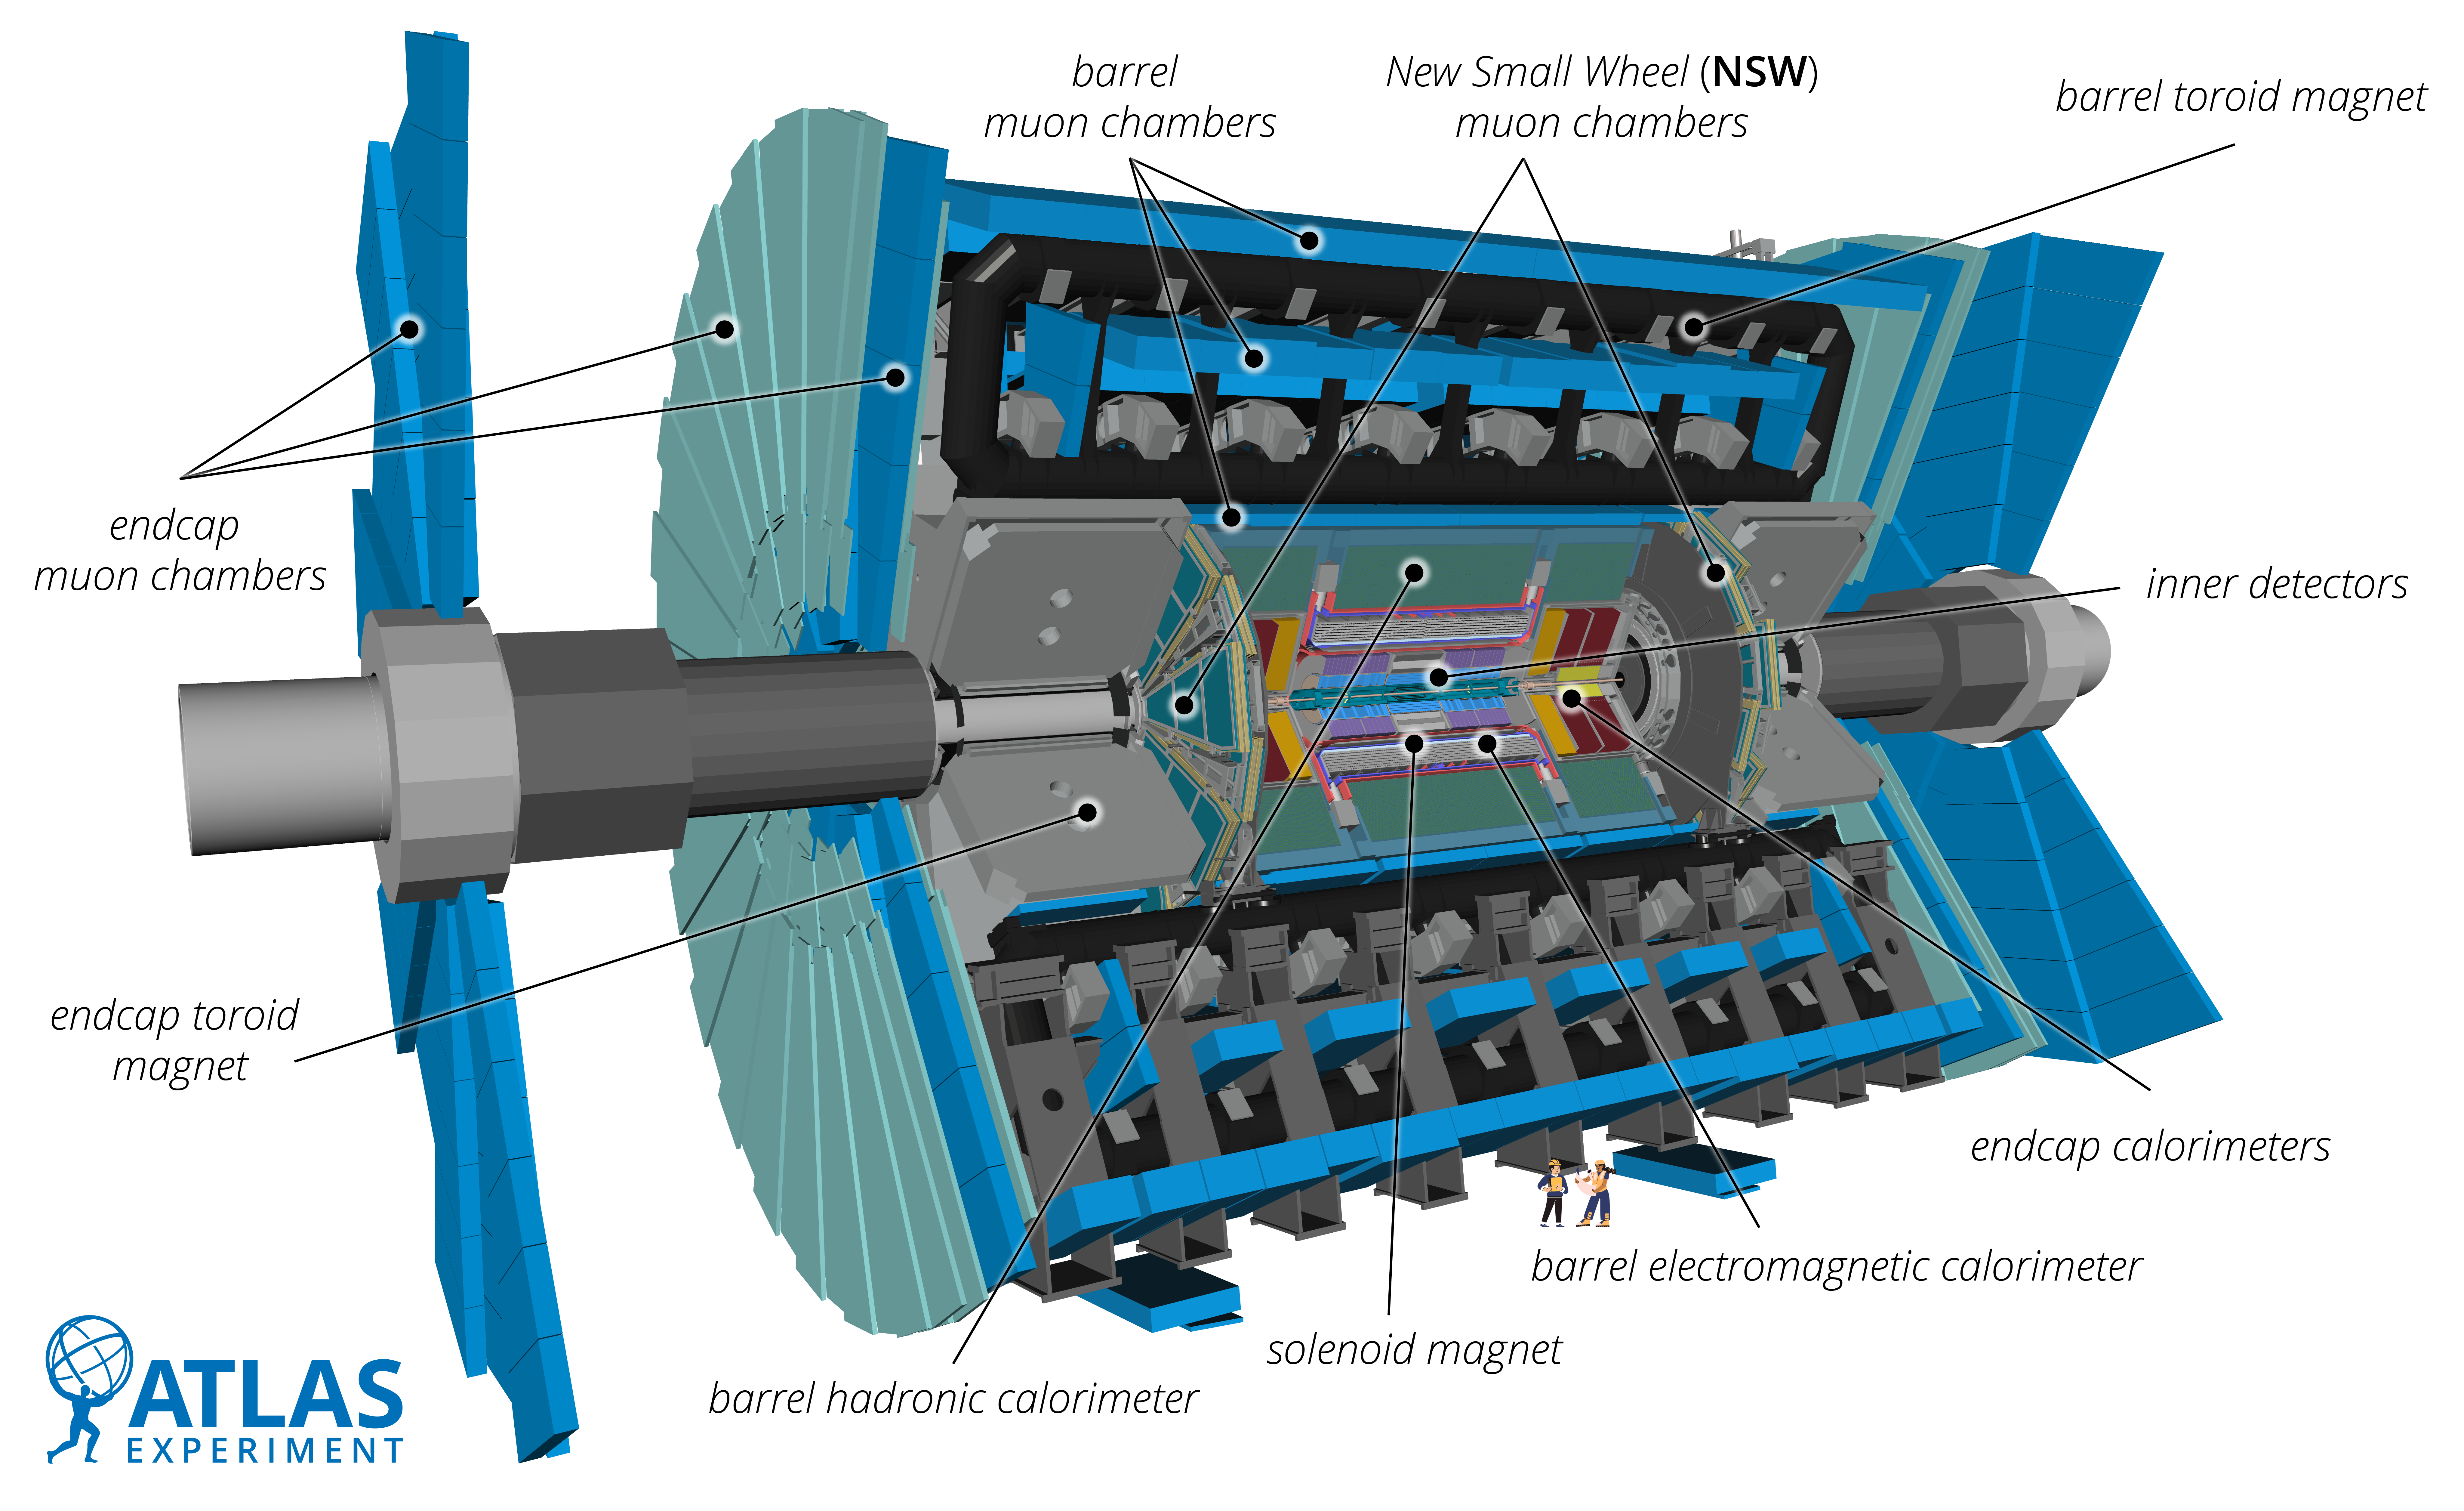
\includegraphics[width=0.8\linewidth]{3_experiment/atlas/ATLAS_full.png}
    \caption{Vista general del detector \ac{ATLAS} y de todos sus subdetectores, incluidos los sistemas añadidos durante el \ac{LS2}~\cite{ATLAS-Diagram}.}
    \label{fig:atlas:atlas:atlas}
\end{figure}

\ac{ATLAS} está construido en capas de subdetectores, cada uno de los cuales está diseñado para tener un papel diferente en la identificación y reconstrucción de las partículas producidas en las colisiones. \ac{ATLAS} proporciona una cobertura hermética alrededor del eje del haz, permitiendo la detección de todas las partículas cargadas generadas en las colisiones en el plano ortogonal al eje del haz. Esto es particularmente importante en las búsquedas de nueva física, que se basan en análisis de balances de momento en el plano ortogonal.

Está formado por múltiples capas, empezando por el componente más interno, el \acf{ID}, que permite reconstruir trazas cerca del tubo del haz. Alrededor del \ac{ID}, hay un solenoide superconductor que crea un campo magnético axial de \(\sim 2\) T para curvar las trazas de las partículas cargadas.
Tras este imán, hay un sistema de dos calorímetros: el \acf{ECAL} y el \acf{HCAL}. El primero se encarga de medir la energía cinética de fotones y electrones, y el segundo mide la energía de los jets.
Las partes más externas del \ac{ATLAS} están constituidas por el \acf{MS}, que proporciona la reconstrucción del momento de los muones que atraviesan las capas internas del detector. Entrelazadas con el \ac{MS}, hay un total de 8 bobinas toroidales que proporcionan un campo magnético total de 4 T para medir el momento de los muones. El campo magnético de los toroides se completa con los toroides en las regiones del end-cap, que también generan un campo magnético de hasta 4 T para los muones que salen en la dirección más próxima al haz.

% El trabajo conjunto de todos los componentes de \ac{ATLAS} permite reconstruir e identificar una gran variedad de partículas con gran precisión. En la \Tab{\ref{tab:atlas:atlas:expected_performance}}, adaptado de \Refn{\cite{ATLAS}}, se da una visión general de las capacidades de diseño de \ac{ATLAS} en términos de resolución de momento y energía.
% Aquí, la resolución está dada primero por un término estocástico, que mide la incertidumbre basada en la interacción de una partícula con el material, seguido de un término de ruido, que da cuenta de las incertidumbres debidas al ruido electrónico en el proceso de lectura.




% \begin{table}[ht!]
%     \caption{Rendimiento esperado del detector \ac{ATLAS}. Las unidades de \pt y \(E\) están en \gev. Extraído de \Refn{\cite{ATLAS}}}
%     \begin{tabular}{|l|c|c|c|}
%         \hline
%         \multirow{2}{*}{\textbf{Componente del detector}}    & \multirow{2}{*}{\textbf{Resolución requerida}}     & \multicolumn{2}{c|}{\textbf{Cobertura en $\eta$}}             \\\cline{3-4} 
%                                                         &                                                   & Offline               & Trigger                        \\ \hline
%         \ac{ID}                                        & \( \sigma_{\pt}/\pt = 0.05\%\pt \oplus 1\%    \)  & \( \pm 2.5 \)            &                                \\ \hline
%         \ac{ECAL}                                  & \( \sigma_{E}/E = 10\%/\sqrt{E} \oplus 0.7\%  \)  & \( \pm 3.2 \)            & \( \pm 2.5 \)                  \\ \hline
%         \ac{HCAL} (jets)                     &                                                   &                          &                                \\
%         $\quad$ barrel y end-cap                       & \( \sigma_{E}/E = 50\%/\sqrt{E} \oplus 3\%    \)  & \( \pm 3.2 \)            & \( \pm 3.2 \)                  \\
%         $\quad$ dirección forward                                  & \( \sigma_{E}/E = 100\%/\sqrt{E} \oplus 10\%  \)  & \( 3.1 < \abseta< 4.9 \) & \( 3.1 < \abseta< 4.9 \)       \\ \hline
%         \ac{MS}                               & \( \sigma_{\pt}/\pt = 10\%\) at \(\pt =1~\tev \)  & \( \pm 2.7 \)            & \( \pm 2.4 \)                  \\
%         \hline
%     \end{tabular}
%     \label{tab:atlas:atlas:expected_performance}
% \end{table}







\subsection{Sistema de coordenadas de ATLAS}

\begin{figure}[ht!]
    \centering
    \includegraphics[width=0.8\linewidth]{3_experiment/atlas/ATLAS_coordinates}
    \caption{Sistema de coordenadas de \ac{ATLAS}~\cite{ATLAS-Diagram}.}
    \label{fig:atlas:atlas:atlas_coordinates}
\end{figure}

El sistema de coordenadas utilizado en \ac{ATLAS}, que se muestra en \Fig{\ref{fig:atlas:atlas:atlas_coordinates}}, se utiliza en toda esta tesis y se describe brevemente a continuación~\cite{ATLAS}.
El origen del sistema de coordenadas está en el punto de interacción nominal, con el eje x positivo apuntando hacia el centro del \ac{LHC}. El plano x-y es perpendicular al eje del haz, definiendo el eje z. Hacia la superficie define el eje y positivo. Alrededor del eje del haz se define un ángulo azimutal $\phi$, y un ángulo polar $\theta$ es el ángulo desde el eje del haz. En lugar de $\theta$ se utiliza la rapidez $y$ que para objetos pesados tiene la forma:
\begin{equation}
    y = \frac{1}{2} \ln[(E+p_z)/(E-p_z)].
\end{equation}
Las diferencias en la rapidez son invariantes a \textit{boosts} a lo largo del eje del haz. Para objetos sin masa o relativistas ($m \ll \vb*{p}$) se utiliza en su lugar la pseudorapidez:
\begin{equation}
    \eta = -\ln(\tan(\theta/2)).
\end{equation}
Para cuantificar la distancia entre dos objetos, se define \DeltaR:
\begin{equation}
    \DeltaR = \sqrt{\Delta\phi^2 + \Delta\eta^2}
\end{equation}
El momento transverso y la energía se definen en el plano x-y, con el momento transverso dado como $\pt = \sqrt{p_x^2 +p_y^2}$.






\subsection{Detector Interno}
\label{subsec:atlas:atlas:id}

\begin{figure}[ht!]
    \centering
    \begin{subfigure}[t]{0.49\linewidth}
        \centering
        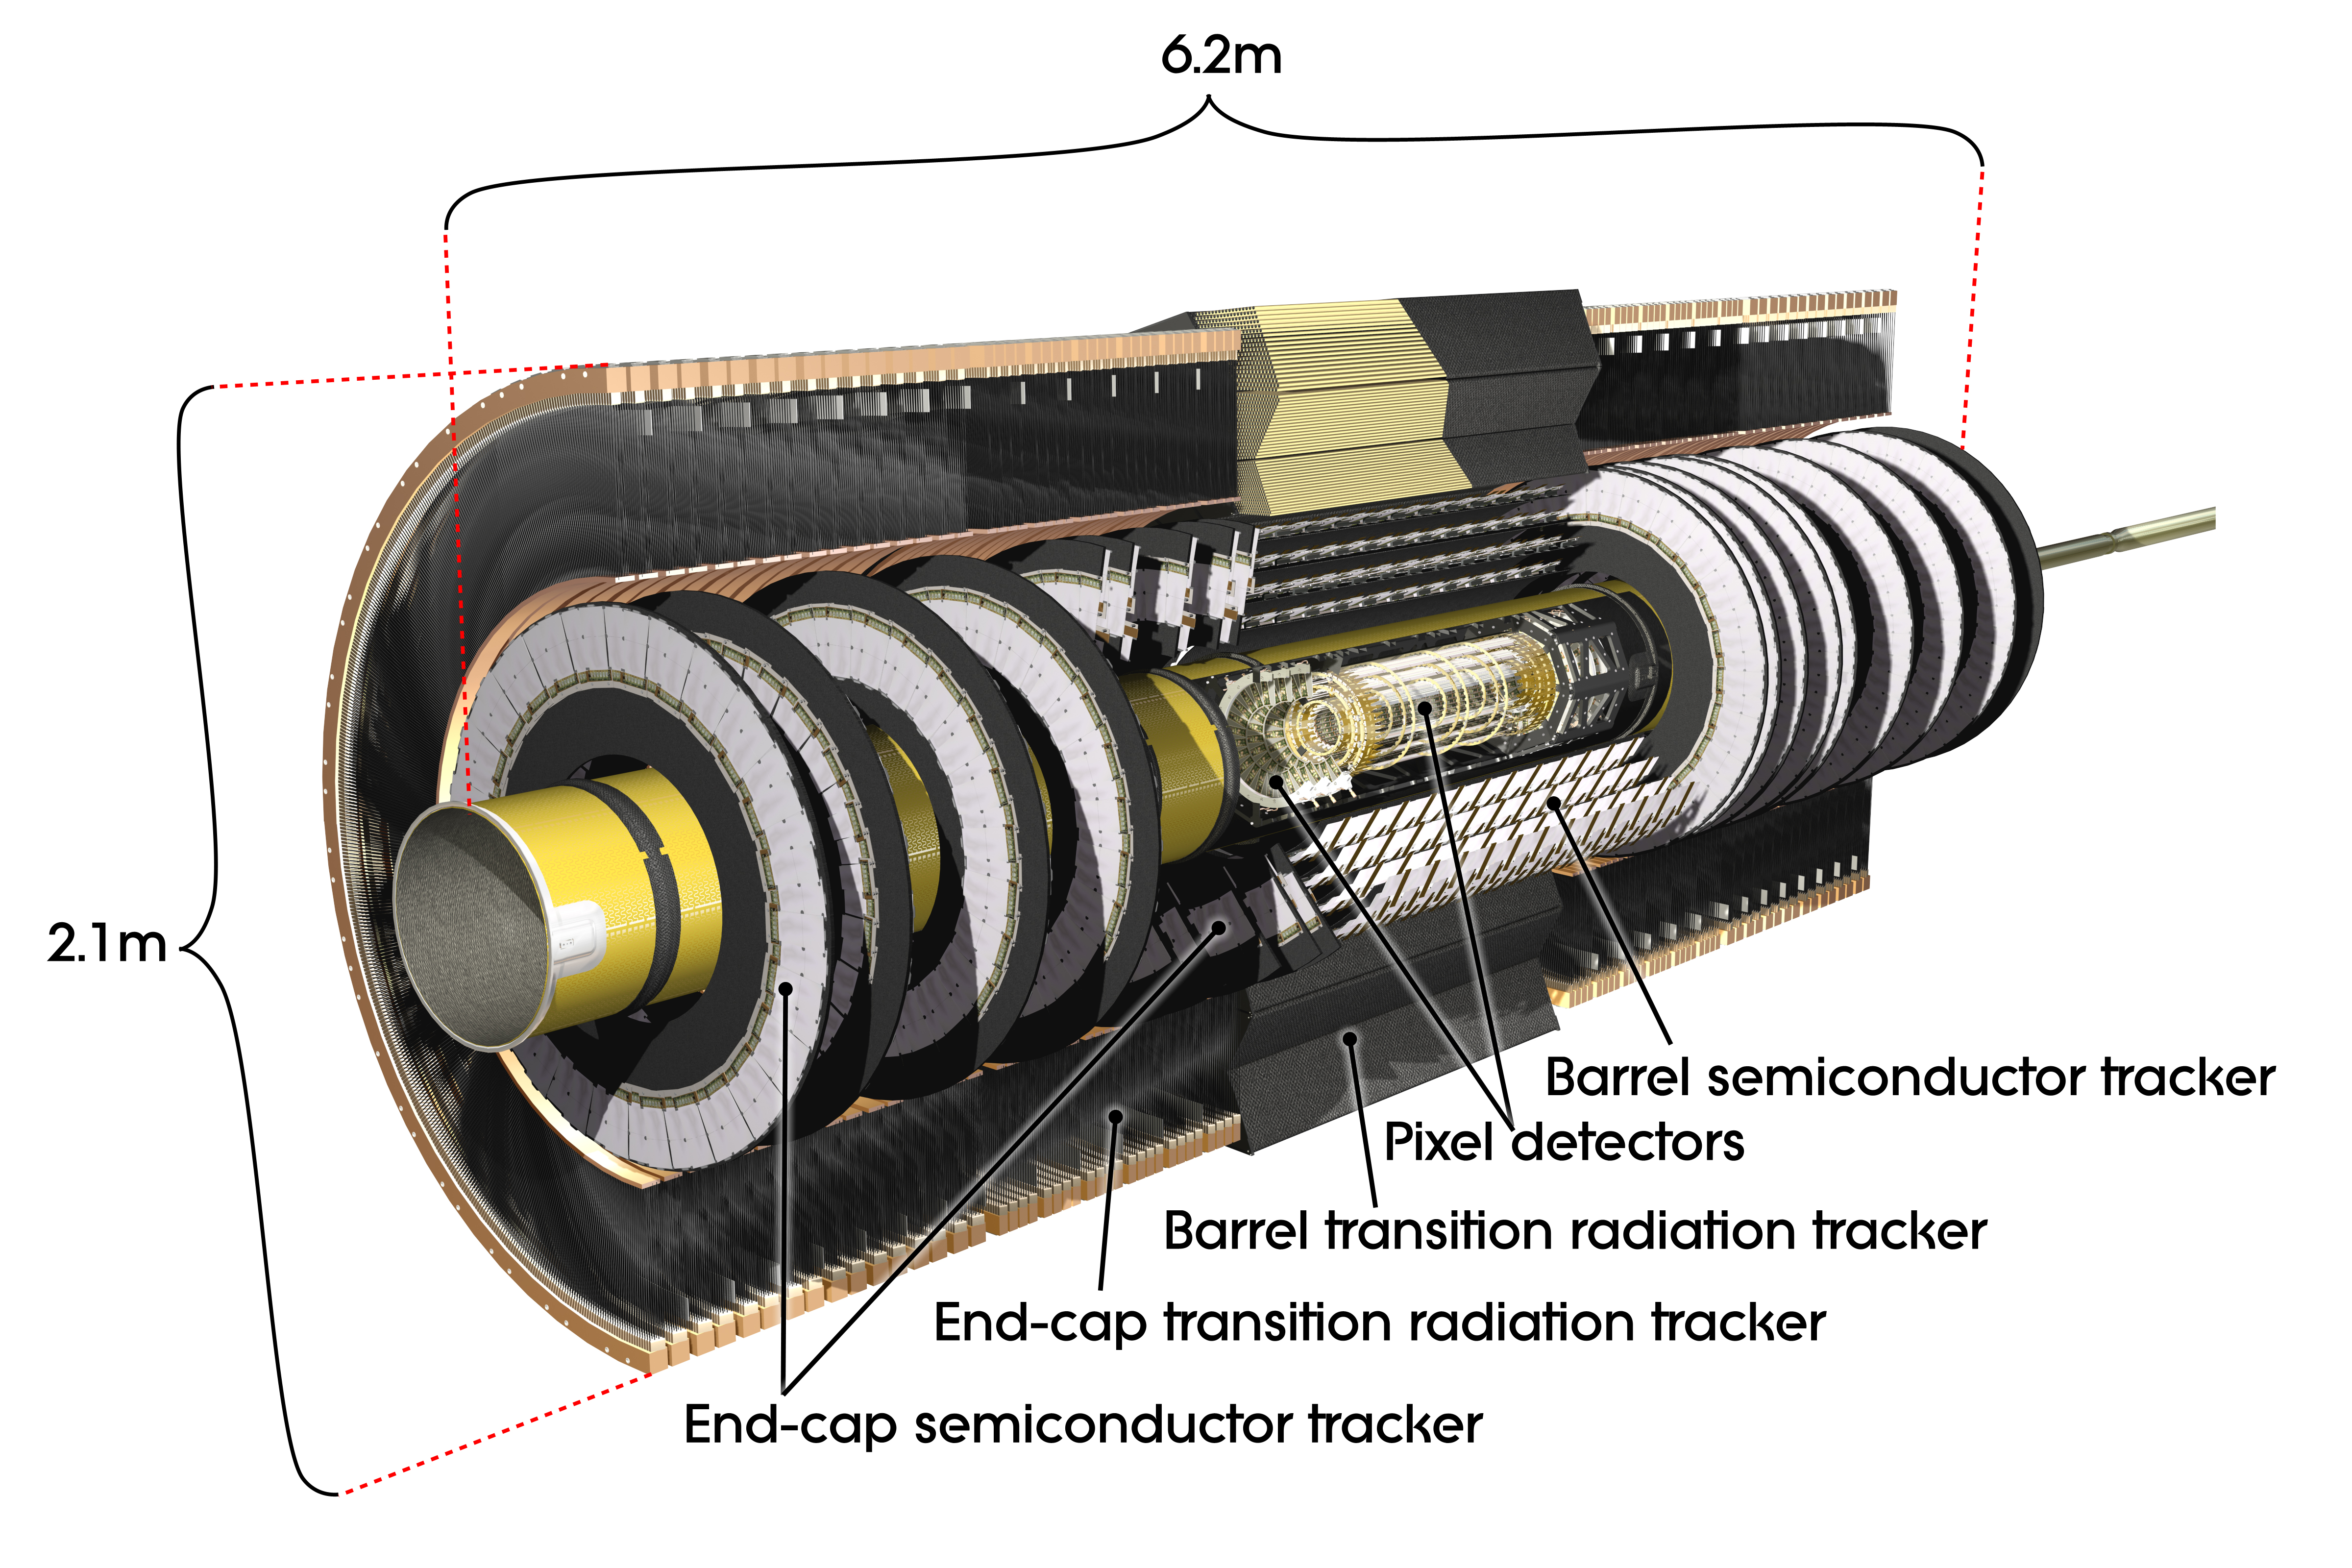
\includegraphics[width=\linewidth]{3_experiment/atlas/inner_detector.jpg}
        \caption{El \ac{ID} con todos sus submódulos en las regiones de barrel y end-cap.~\cite{ATLAS-InnerDetector}.}
        \label{fig:atlas:atlas:atlas_inner_detector:general}
    \end{subfigure}
    \hfill
    \begin{subfigure}[t]{0.49\linewidth}
        \centering
        \includegraphics[width=0.8\linewidth]{3_experiment/atlas/inner_detector_layers}
        \caption{Capas del \ac{ID} mostrando su distancia al haz~\cite{ATLAS-InnerDetector}.}
        \label{fig:atlas:atlas:atlas_inner_detector:layer_radius}
    \end{subfigure}
    \caption{Diagramas del \ac{ID} que muestran los diferentes submódulos, con sus correspondientes dimensiones.}
    \label{fig:atlas:atlas:atlas_inner_detector}
\end{figure}

El esquema de un corte transversal del \acf{ID} \cite{ATLAS-ID-TDR} se muestra en la \Fig{\ref{fig:atlas:atlas:atlas_inner_detector}}, resaltando la distancia de cada subsistema respecto al tubo del haz. La parte más interna del \ac{ID} se denomina \ac{IBL}, seguido de tres capas de detectores de píxeles. A 299 mm de distancia radial del tubo del haz, cuatro capas de módulos del \ac{SCT} se sitúan antes del \ac{TRT}, que amplía el tamaño total del \ac{ID} a un radio de 1082 mm. El \ac{ID} permite la reconstrucción de las trazas de partículas en un rango de $\abseta < 2.5$.


La función del \ac{ID} es la reconstrucción de las trazas de las partículas cargadas para determinar su carga y momento. Está inmerso en un campo magnético de 2 T generado por el sistema magnético del solenoide de \ac{ATLAS}, que curva las trayectorias de las partículas cargadas. El radio de curvatura es proporcional al momento de la partícula y su dirección distingue las cargas positivas de las negativas. Las trazas de las partículas detectadas permiten reconstruir los vértices de colisiones primarios, lo cual es importante para distinguir las colisiones de \textit{pile-up} (término que será descrito más adelante) de las colisiones de interés, y los vértices secundarios de decaimiento producidos por partículas de vida media larga, lo que es crucial para la identificación de, por ejemplo, mesones \(B\) o leptones \(\tau\). A continuación, se brinda una breve descripción de cada parte del \ac{ID}.


\paragraph{\acf{IBL}}
Después del Run-1, durante el \ac{LS1} en el período de 2013-2014, el sistema detector de píxeles fue sometido a mantenimiento y actualizaciones. Dentro de este conjunto de actualizaciones, una cuarta capa de píxeles a 3.3 cm de distancia del tubo del haz fue instalada~\cite{ATLAS-IBL-TDR,ATLAS-IBL-proceedings} y ha permitido mejoras significativas en la reconstrucción de vértices de interacción y la identificación de jets iniciados por quarks \(b\).


\paragraph{Detector de Píxeles}
La capa de píxeles más interna, el \ac{IBL}, está rodeada por tres capas de detectores de píxeles, dispuestas alrededor del tubo del haz~\cite{ATLAS-Pixel-DesignPerformance,ATLAS-Pixel-Performance-Proceedings}. El método de detección de partículas cargadas es la medición de cargas inducidas depositadas en una capa de silicio, producto de la ionización. La primera capa se encuentra a una distancia de 50.5 mm del centro del tubo del haz. Como se puede ver en la \Fig{\ref{fig:atlas:atlas:atlas_inner_detector:general}}, en la región del end-cap los detectores de píxeles consisten en 3 discos alrededor del tubo, aumentando la longitud del detector de píxeles del \ac{ID} a 1.4 m a lo largo del eje del haz. El detector de píxeles consta de un total de 1744 módulos de píxeles con un tamaño nominal de $50 ~\mu m \times 400 ~\mu m$ en el plano $(\phi, z)$, que comprenden más de 80 millones de canales de lectura.  
La parte de píxeles y \ac{IBL} del detector \ac{ATLAS} es crucial para la reconstrucción de trazas, ya que proporciona 4 puntos de medición (\textit{hits}) en todo el rango de cobertura de pseudorapidez ($|\eta| < 2.5.$).  

\paragraph{\acf{SCT}}
El detector de píxeles y \ac{IBL} se encuentran dentro de los módulos del \ac{SCT}~\cite{ATLAS-SCT}.  
Al igual que los módulos detectores de píxeles, los módulos del \ac{SCT} están basados en semiconductores, dispuestos en capas cilíndricas alrededor del tubo del haz en la región del barrel, formando discos en los end-caps. Dado que los módulos del \ac{SCT} sólo proporcionan una localización precisa a lo largo de un eje, se combinan dos módulos uno detrás de otro y rotados entre sí para obtener información espacial bidimensional. En el barrel hay cuatro capas y en los end-caps, nueve discos en cada lado (véase la \Fig{\ref{fig:atlas:atlas:atlas_inner_detector:general}}). Incluyendo los discos de los end-caps, el \ac{SCT} se extiende hasta $|z| < 2735~mm$.

\paragraph{\acf{TRT}}
La última parte del \ac{ID} es el \ac{TRT}~\cite{ATLAS-TRT-DesignPerformance}, el cual en la región barrel se extiende de 554 mm a 1082 mm de distancia radial. Este detector se compone de tubos detectores de 4 mm de diámetro, dispuestos en paralelo al tubo del haz en la región barrel, y radialmente en los end-caps. En el rango de $|\eta| < 2.0$, se sitúan tres anillos en el barrel y 18 unidades en los end-caps, proporcionando típicamente 36 impactos por traza. Los tubos están entrelazadas con fibras de polipropileno, que cuando las partículas las atraviesan, crean la radiación de transición. En el interior de los tubos hay un fino cable de tungsteno que recoge las cargas. El nivel de radiación y las cargas recogidas en cada tubo pueden utilizarse para discriminar entre electrones y piones cargados. El \ac{TRT} sólo ofrece información espacial en el plano $(R-\phi)$, y no se puede extraer información en la dirección z debido a la orientación de estos tubos. Hay un total de aproximadamente 50000 tubos en la región del barrel, mientras que en los end-caps se sitúan aproximadamente 250000 tubos.








\subsection{Calorímetros}

\begin{figure}[ht!]
    \centering
    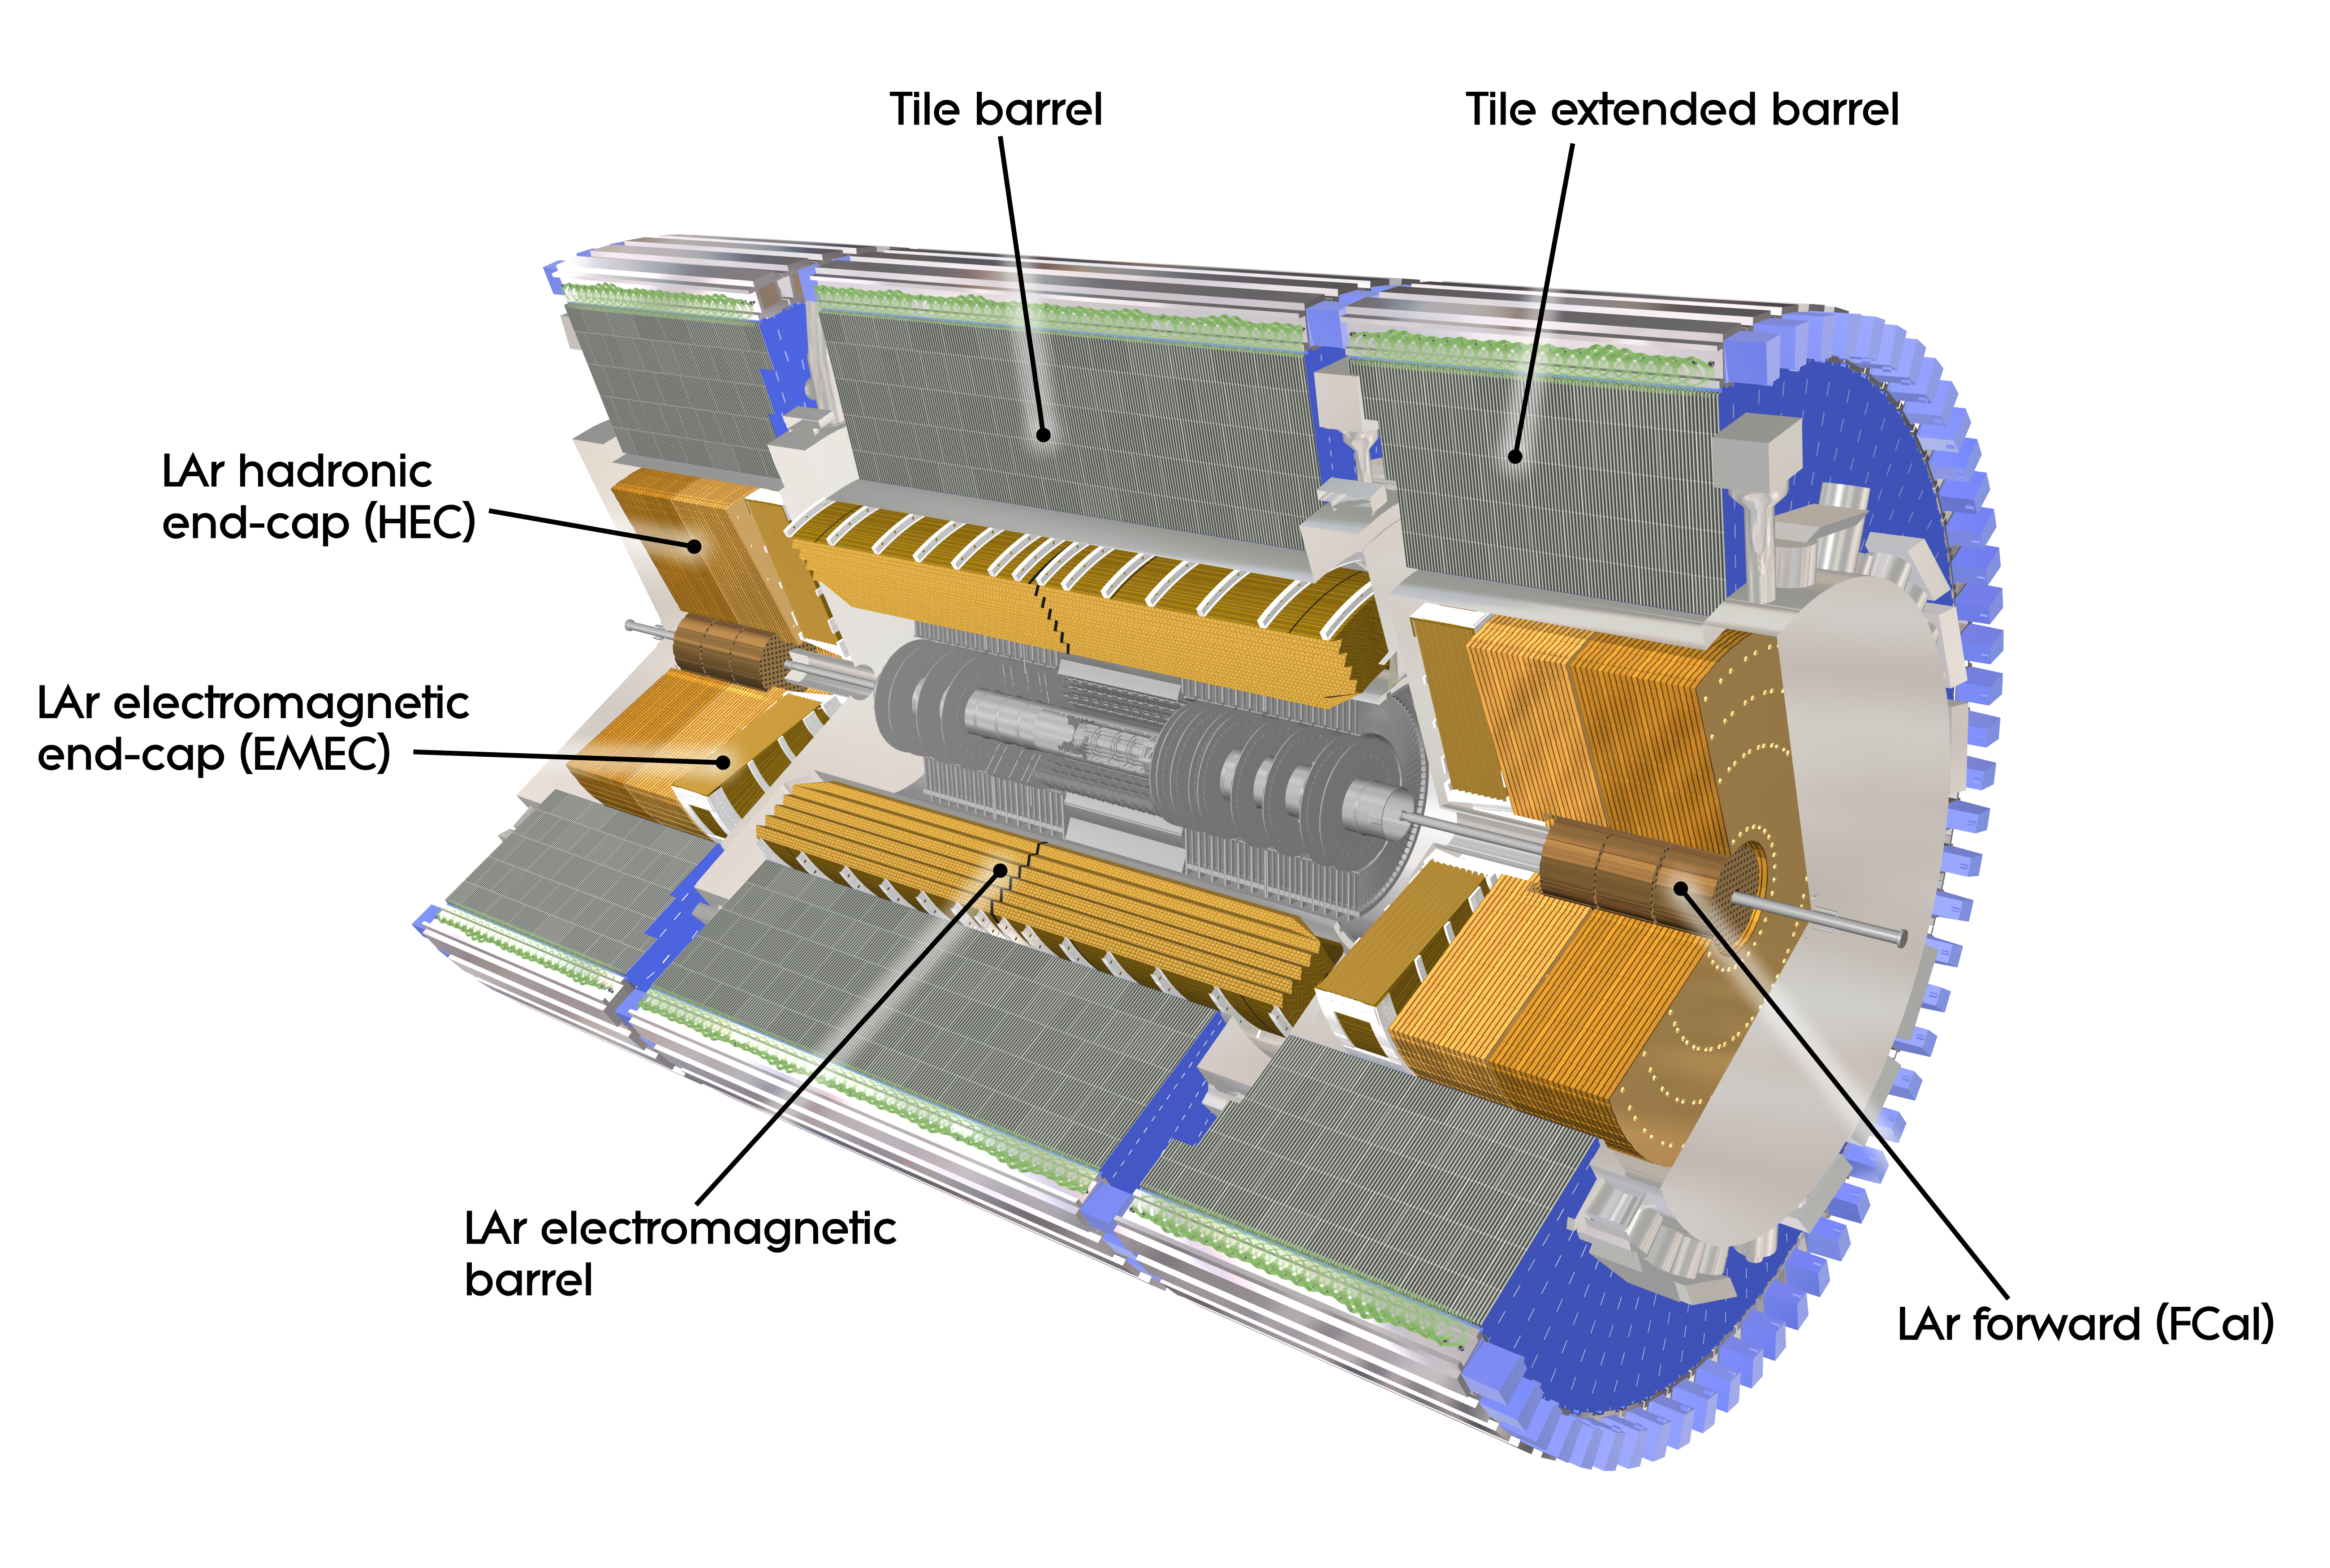
\includegraphics[width=0.8\linewidth]{3_experiment/atlas/calorimenters.jpg}
    \caption{Sistema de calorímetros de \ac{ATLAS}, mostrando el \acf{ECAL} y el \acf{HCAL}~\cite{ATLAS-Calorimeter-Diagram}.}
    \label{fig:atlas:atlas:atlas_calorimeters}
\end{figure}

El sistema \ac{ID} está rodeado por dos calorímetros: el \acf{ECAL} y el \acf{HCAL}, como se muestra en la \Fig{\ref{fig:atlas:atlas:atlas_calorimeters}}. Estos calorímetros están diseñados para medir la energía y la posición de las partículas incidentes, a través de la energía depositada por las cascadas de partículas secundarias producidas por las incidentes. Cubre todo el rango \(\phi\) y hasta el \(\abseta<4.9\), con una granularidad más fina en la región que coincide con el \ac{ID}.
El sistema de calorímetro permite discriminar entre fotones y electrones de hadrones (jets). Además, permite medir el desequilibrio energético (gracias a su cobertura total y hermiticidad) y proporciona al sistema de trigger la información necesaria para la selección de eventos.

Ambos calorímetros son denominados calorímetros de muestreo, con capas alternas de material absorbente y activo. La capa absorbente desencadena una lluvia de partículas consecutivas con el material detector, la capa activa detecta la señal.
El desarrollo de la lluvia y sus propiedades son de vital importancia para la identificación de las partículas, como se verá más adelante.
Dos magnitudes importantes en relación con los calorímetros son la longitud de radiación, $X_0$, y la longitud de interacción $\lambda$. La longitud de radiación se refiere a la distancia después de la cual la energía de una partícula (electrones por ejemplo) se ha reducido a \(1/e\) de su energía inicial. La longitud de interacción describe el camino libre medio antes de que se produzca una interacción hadrónica.

La resolución de diseño del sistema sobre la energía calorimétrica viene dada por
\begin{equation}
    \frac{\sigma(E)}{E} = 
    \frac{a}{\sqrt{E}} \oplus b \oplus \frac{c}{E}
\end{equation}
donde \(\oplus\) significa que los términos se suman en cuadratura. El término estocástico \(\frac{a}{\sqrt{E}}\) está relacionado con las fluctuaciones en los desarrollos de la lluvia, el término constante \(b\) tiene en cuenta las inhomogeneidades del detector, y el último término está asociado con el ruido electrónico y es proporcional a \(\frac{1}{E}\). El valor de los coeficientes \(a\) y \(b\) depende de los objetos incidentes. Para el caso de los electrones en el \ac{ECAL}, \(a\sim 10\%~\gev^{1/2}\) y \(b~\sim 0.7\%\), mientras que los de los piones cargados en el centro del detector son \(a~\sim50\%~\gev^{1/2}\) y \(b\sim5\%\) \cite{ATLAS-Calorimeters-PerformanceRun2}.



\subsubsection{\acf{ECAL}}
\label{subsubsec:atlas:atlas:cals:ecal}

El \ac{ECAL} está especializado en la detección de electrones, positrones y fotones, que depositan su energía en lluvias relativamente densas: electrones energéticos que irradian fotones Bremsstrahlung, mientras que los fotones energéticos se convierten en pares electrón-positrón al atravesar el material denso.
El material absorbente está hecho de plomo (Pb) con láminas de acero inoxidable, mientras que el \ac{LAr} se utiliza como material activo con electrodos de cobre y kaptón para la lectura.


El calorímetro tiene una geometría de acordeón que proporciona una simetría completa \(\phi\) sin fisuras azimutales.
Está dividido en dos medios barriles que cubren la región central del detector (\(\abseta<1.475\)), con un pequeño hueco (4 mm) en $z = 0$ y una tapa final a cada lado del haz (\(1.375<\abseta<3.2\)).
La región de transición entre el barrel y end-cap se denomina región \textit{crack}, y la mayoría de los análisis físicos que utilizan el \ac{ECAL} requieren que los fotones y electrones se encuentren fuera de ella.
Además el \ac{LAr} se utiliza para las tapas de los calorímetros hadrónicos, así como en el \acf{FCAL} ($3.1 < \eta < 4.9$).

El grosor de \ac{ECAL} es superior a 22 longitudes de radiación (\(X_0\)) en la región del barrel, mientras que es superior a \(24 X_0\) en la región de end-caps. En el caso de los fotones, la distancia a la que la energía baja a \(1/e\) es de \(9/7 X_0\), por lo que toda la energía electromagnética del fotón se deposita en el \ac{ECAL}, y sólo una pequeña parte llega al \ac{HCAL}.

El modo de medición es el siguiente. Las partículas incidentes interactúan con el medio absorbente (Pb), iniciando una lluvia de partículas cargadas y neutras. Las partículas cargadas ionizan el \ac{LAr} y los electrodos recogen los electrones producidos en el proceso de ionización. La señal total del medio activo es entonces proporcional a la energía real total de la partícula incidente.

\begin{figure}[ht!]
    \centering
    \includegraphics[width=0.8\linewidth]{3_experiment/atlas/ecal_cells}
    \caption{Segmento del \ac{ECAL} mostrando la disposición de las capas y celdas del calorímetro. Además, se muestran las dimensiones de las celdas en cada capa~\cite{ATLAS}.}
    \label{fig:atlas:atlas:cals:ecal:ecal_cells}
\end{figure}

\begin{figure}[ht!]
    \centering
    \includegraphics[width=0.46\linewidth]{3_experiment/atlas/ecal_radiation_lengths1}
    \includegraphics[width=0.46\linewidth]{3_experiment/atlas/ecal_radiation_lengths2}
    \caption{Longitudes de radiación en función de \abseta para cada capa del \ac{ECAL}~\cite{ATLAS}.}
    \label{fig:atlas:atlas:cals:ecal:ecal_radiation_length}
\end{figure}

Dentro de la región aceptada para las medidas de precisión (\(\abseta<2.5\) excluyendo el crack), el \ac{ECAL} se segmenta en tres capas longitudinales, mostradas en la \Fig{\ref{fig:atlas:atlas:cals:ecal:ecal_cells}}.
La primera capa consiste en bandas de granularidad fina (también llamada \textit{strip layer}) que ayuda a discriminar entre fotones aislados y pares de fotones espacialmente cercanos procedentes de decaimientos \(\pizero\to\gamma\gamma\). Esta capa tiene un espesor constante de \(\sim 6 X_0\) en función de \(\eta\) (véase la \Fig{\ref{fig:atlas:atlas:cals:ecal:ecal_radiation_length}}), y proporciona una medida precisa de \(\eta\).
Para los fotones y electrones de alta energía, la mayor parte de su energía se recoge en la segunda capa, que tiene una granularidad lateral de \(0.025 \times 0.025\) en \((\eta, \phi)\) y un espesor de \(\sim 24 X_0\).
La tercera capa recoge la energía depositada por las colas de la lluvia electromagnética, con un espesor que varía entre 2 y 12 \(X_0\).
También hay un \textit{presampler} (no se muestra en las figuras), que cubre la región \(\abseta<1.8\) que mejora la medición de la energía para las partículas que comienzan la lluvia antes de entrar en el calorímetro.




\subsubsection{\acf{HCAL}}



Tres capas de calorímetro hadrónico rodean el \ac{ECAL} y proporcionan discriminación adicional para electrones y fotones al medir la energía hadrónica. El \ac{HCAL} se extiende en pseudorapidez hasta \(\abseta<4.9\), permitiendo cubrir prácticamente la totalidad del ángulo sólido desde el punto de interacción. En la región del barrel (\(\abseta<1.7\)) se encuentra el primer calorímetro, el \textit{Tile calorimeter}, un calorímetro de muestreo que utiliza acero como material absorbente y tejas centelladoras como material activo~\cite{ATLAS-Tile-TDR}. Está dividido en dos partes: \(\abseta<1.0\) y \(0.8<\abseta<1.7\). Las tejas centelleadoras están dispuestas de una forma periódica y están conectadas a una fibra óptica que transporta la luz producida por las partículas que pasan a un tubo fotomultiplicador. Este arreglo se extiende, en \(R\), de 2.28 a 4.25 m. En la región del end-cap (\(1.5<\abseta<3.2\)) hay un calorímetro de muestreo hadrónico, el \acf{HEC}, con placas de cobre como absorbente y argón líquido como material activo. Cada lado del endcap consiste en dos ruedas, una detrás de la otra con las placas planas de Cu dispuestas perpendicularmente al eje del haz, con un radio de 2.3 m. Finalmente está el \ac{FCAL}, un calorímetro de muestreo que extiende la cobertura del sistema hasta \(\abseta<4.9\), coaxial al eje del haz y situado a 4.7 m a cada lado del punto de interacción. El material principal de los módulos es el \ac{LAr} (con cobre o tungsteno), y aunque no se utiliza para mediciones de precisión, proporciona información para el cálculo de la energía transversa faltante y la reconstrucción de jets en regiones muy cercanas al eje del haz.

El \ac{HCAL} tiene un espesor superior a \(7.7~\lambda\) en la región del barrel (\(9.7~\lambda\) en total si se cuenta el \ac{ECAL}). Análogamente a la longitud de radiación mencionada para el \ac{ECAL}, se puede definir la longitud de interacción hadrónica como la distancia media a lo largo de la cual la energía de un hadrón se reduce a \(1/e\) de su energía inicial. Así, toda la energía con la que los hadrones llegan al \ac{HCAL} se deposita allí.





\subsection{\acf{MS}}

\begin{figure}[ht!]
    \centering
    \includegraphics[width=0.6\linewidth]{3_experiment/atlas/muon_detector}
    \caption{Diagrama del \acf{MS}~\cite{ATLAS}.}
    \label{fig:atlas:atlas:muon_spectrometer:muon_spectrometer}
\end{figure}

Los muones de alto \pt generados en el punto de interacción tienen un poder de penetración muy elevado y son poco interactivos. Por lo tanto, el \ac{MS} \cite{ATLAS-Muon-TDR} está situado en la parte más externa del detector \ac{ATLAS}, insertado dentro del campo magnético de 4 T generado por los imanes toroidales del barrel y end-caps, y está diseñado para obtener medidas de posición y momento con alta precisión de los muones de alto \pt en un rango de \abseta de \(\abseta<2.7\). Se trata del mayor subdetector y el que da a \ac{ATLAS} su tamaño. Este subdetector se muestra en la \Fig{\ref{fig:atlas:atlas:muon_spectrometer:muon_spectrometer}}, destacando los subsistemas.

El \ac{MS} se compone de diferentes tipos de cámaras de detección (véase la \Fig{\ref{fig:atlas:atlas:muon_spectrometer:muon_spectrometer}}). Los \acp{MDT} son responsables de la mayoría de las medidas de precisión y cubren el rango de pseudorapidez hasta \(\abseta<2.7\). Funcionan de forma similar al \ac{TRT}, con tubos llenos de un gas ionizante y un ánodo central que recoge los electrones producidos, y el tiempo de deriva está asociado a la distancia a la traza dejada por la partícula. En la región del endcap se encuentran las \acp{CSC} que tienen una alta resolución espaciotemporal y una cobertura de \(\abseta>2.0\). Estas cámaras funcionan midiendo la carga depositada en un ánodo como resultado de la cascada de electrones creada cerca de él. Las \acp{RPC} proporcionan una estimación rápida del momento de los muones a nivel de trigger con una cobertura de \(\abseta<1.05\)\footnote{Durante el \ac{LS2}, la capa del end-cap ma\'s interna ha sido reemplazada por las \acp{NSW}~\cite{ATLAS-NSW}. Presenta MicroMegas como rastreadores de precisión ya que proporcionan un mejor rendimiento a las altas tasas esperadas en las futuras operaciones del LHC.}. Las \acp{RPC} miden la descarga entre dos placas resistivas paralelas sometidas a una elevada diferencia de potencial, siguiendo la ionización del volumen de gas interno causada por el paso de muones energéticos. Por último, en la región del endcap, se encuentran los \acp{TGC}, de función similar a los \acp{CSC}. También proporcionan información al sistema de trigger en esta región y tienen una cobertura de \(\abseta<2.4\).

Si los hits en el \ac{ID} y el \ac{MS} se pueden asociar a un solo muón, se obtiene una muy buena resolución del momento de hasta
\begin{equation}
    \frac{\sigma(\pt)}{\pt} = 
    0.02\% \cdot \pt~[\gev] \oplus 2\%,
\end{equation}
la cual se degrada si sólo se identifica una traza en uno de los dos sistemas.






\subsection{El sistema de Trigger}



El sistema de trigger de \ac{ATLAS}~\cite{ATLAS-Trigger-Performance-2010,ATLAS-Trigger-Performance-2015,ATLAS-Trigger-Performance-Run2} utiliza información del detector para rechazar eventos que no son de interés para el programa de \ac{ATLAS} (colisiones \textit{soft}, por ejemplo), reduciendo la frecuencia de eventos de 40 MHz (frecuencia de cruce de bunches mencionada en la \Sect{\ref{sec:atlas:LHC}}) a alrededor de 1.5 kHz. Es necesario enfatizar aquí el papel central del sistema de trigger para el correcto funcionamiento de todo el experimento, siendo el responsable de decidir qué eventos se almacenan para su posterior análisis, que podría llevar, por ejemplo, a un descubrimiento. Para lograr tal reducción en la frecuencia de eventos y, al mismo tiempo, tener una alta eficiencia en la selección de los de interés, el sistema de trigger se compone de dos niveles consecutivos capaces de realizar una identificación de partículas cada vez más compleja; un primer nivel de trigger basado en hardware, el \acf{L1}, y luego un trigger de alto nivel basado en software, el \acf{HLT}. Cada nivel permite analizar los eventos con mayor detalle, aumentando la precisión de los criterios de selección y la complejidad de los algoritmos utilizados.


\subsubsection{\acf{L1}}

La decisión del trigger comienza con el \ac{L1}, basado en hardware~\cite{ATLAS-L1Trigger}, que identifica lo que se conoce como \ac{ROI}. La \ac{ROI} consiste en celdas vecinas en los \ac{ECAL} y \ac{HCAL}, y se define a partir de la posición en el calorímetro de cada objeto encontrado en un evento potencialmente interesante, que se extiende como un cono desde el punto de interacción a lo largo del detector.
En cuanto a los muones, toma la información leída por el \ac{MS}, más concretamente por el \ac{TGC} y el \ac{RPC}, y permite obtener una estimación rápida del \pt del muón.
El \ac{L1} también tiene una componente que permite tener en cuenta los requisitos topológicos, como las selecciones de masa invariante y las medidas de distancia, denominado el \ac{L1Topo}.

El diseño del \ac{L1} permite tener una aceptabilidad en el rango de \(\abseta<2.5\) para electrones, fotones, muones y taus, hasta \(\abseta<3.2\) para jets, y \(\abseta<4.9\) para el cálculo del momento transverso faltante.
Utilizando las \acp{ROI}, el trigger \ac{L1} debe tomar la decisión de guardar o descartar el evento, reduciendo la tasa de eventos de 40 MHz a menos de 100 kHz en aproximadamente \(2.5~\mu s\), tiempo determinado en parte por el tamaño limitado de los buffers de memoria y en parte por el tiempo que tardan los muones producidos en el evento en llegar al \ac{MS}. Esta decisión final la toma el \ac{CTP}, y luego pasa las \acp{ROI} al siguiente nivel de trigger: el \ac{HLT}.



\subsubsection{\acf{HLT}}


Cuando un evento es aceptado por el \ac{L1}, el \ac{HLT}~\cite{ATLAS-HLTTrigger} ejecuta una secuencia de algoritmos a partir de las \acp{ROI} definidas por el \ac{L1}, y permite reducir la tasa de eventos que se almacena a 1.5 kHz en 0.2 s.
La reconstrucción e identificación de partículas candidatas en el \ac{HLT} se evalúa en una secuencia de pasos donde se aplican diferentes algoritmos.
Si la selección falla en un determinado paso, los pasos siguientes ya no se ejecutan para ahorrar tiempo de ejecución.
En el \ac{HLT}, los algoritmos se agrupan en conjuntos de algoritmos de reconstrucción rápida que se ejecutan en primer lugar y, a continuación, se ejecuta un conjunto de algoritmos de reconstrucción de precisión similares a los utilizados \textit{offline}.
Los algoritmos de reconstrucción rápida utilizan la información del calorímetro y de las trazas del \ac{ID} sólo dentro de la \ac{ROI} para realizar la selección e identificación de candidatos, y llevar a cabo el rechazo del fondo lo más rápido posible.
Si la partícula candidata supera los criterios definidos por la selección de reconstrucción rápida, se ejecutan los algoritmos de selección de precisión. Estos tienen acceso a la información del detector fuera de la \ac{ROI}, con la máxima granularidad e incluyendo detalles sobre la calibración energética del calorímetro, la alineación del subdetector y el mapeo del campo magnético.

La secuencia exacta y el tipo de algoritmos considerados en el \ac{HLT} se definen en el \textit{menu} del trigger. Esto comprende una base de datos de triggers, cada uno de los cuales define una secuencia de algoritmos y los requisitos de estos algoritmos para que un evento pase el \ac{HLT}.

Los requisitos de trigger se diseñan de forma tal que la tasa global del \ac{HLT} no supere 1 kHz. En algunos casos, incluso la reducción de la tasa de eventos conseguida mediante los algoritmos del \ac{HLT} para los requisitos de trigger deseados, como los trigger para objetos con bajo momento, es demasiado alta. Para mantener la tasa general del \ac{HLT} por debajo de 1 kHz en estos casos, los triggers pueden seguir incluyéndose en el menú, pero con una preescala. Un preescalado es un escalado artificial del trigger, que sólo acepta la N-ésima decisión de trigger si el factor de preescalado es N. Esto permite que los triggers con una alta tasa sigan recogiendo eventos.

Los algoritmos del \ac{HLT} se ejecutan en aproximadamente 40.000 núcleos de CPU. Además, la construcción parcial de eventos se utiliza para análisis a nivel de trigger, para el monitoreo del detector y las calibraciones del subsistema detector. Finalmente, los eventos aceptados por el \ac{HLT} se almacenan y se distribuyen, disponibles \textit{offline} para cualquier estudio o análisis.






\FloatBarrier
\section{Toma de datos durante el Run-2}
\label{sec:atlas:runs}


El funcionamiento del \ac{LHC} se organiza en distintos períodos conocidos como \textit{runs}.
% Cada run suele durar varios años y se caracteriza por condiciones experimentales específicas, como la energía a la que colisionan los protones y la intensidad de los haces.
Desde su puesta en marcha, se pueden distinguir los siguientes runs: Run-1 (2010-2013) operó a energías de colisión de hasta 8 TeV, Run-2 (2015-2018) a 13 TeV, y Run-3 (2022-presente) a 13.6 TeV. Cada período de toma de datos, una vez que el \ac{LHC} anuncia haces estables, se divide en \ac{LB} de aproximadamente dos minutos. En cada \ac{LB}, la luminosidad instantánea es prácticamente constante y las condiciones del haz son estables. Debido a la alta complejidad del \ac{LHC} y del detector \ac{ATLAS}, se espera que haya ineficiencias en los detectores y subdetectores y/o en la cadena de adquisición de datos. Durante cada run, cada parte del \ac{ATLAS} es monitoreada y cualquier falla o problema es registrado, incluyendo componentes inactivos, o problemas en el haz del \ac{LHC}.

Para garantizar la alta calidad de los datos, libres de defectos significativos, los \ac{LB} y los rangos dentro de ellos que superan todos los criterios de calidad se compilan en \ac{GRL}. Las listas se elaboran y distribuyen de forma centralizada, con el fin de proporcionar a cualquier grupo de \ac{ATLAS} la misma colección de \acp{LB}. Dado que durante los períodos de tomas de datos están disponibles diferentes partes del detector (en un run óptimo, todos los subdetectores están disponibles), hay múltiples \acp{GRL} disponibles para utilizar. Cada análisis, entonces, selecciona qué \ac{GRL} utilizar dependiendo de su tolerancia a las fallas de los subdetectores.

La presente tesis utiliza datos recolectados por \ac{ATLAS} de colisiones \pp del \ac{LHC} durante el Run-2 (2015-2018), a una energía del centro de masa de \(\sqrt{s} = 13~\tev\). Durante este run, el \ac{LHC} entregó un total de \(156~\ifb\), de los cuales \ac{ATLAS} recolectó \(147~\ifb\). La luminosidad integrada total disponible para análisis de física es de \(140.07~\ifb\)\footnote{Las primeras medidas y \ac{GRL} iniciales sólo brindaban un total de \(139~\ifb\) disponibles para análisis}, como se ve en la \Fig{\ref{fig:atlas:runs:lumi_run2}}. La incertidumbre en la luminosidad integrada combinada para el Run-2 es de \(0.83\%\)~\cite{ATLAS-Lumi-Run2}, obtenida usando el detector LUCID-2~\cite{ATLAS-LUCID2}.
Hasta el momento, combinando los años 2022, 2023 y 2024 de toma de datos del Run-3, se recogieron 159 \ifb de datos, mostrados en la \Fig{\ref{fig:atlas:runs:lumi_run3}}~\cite{ATLAS-Lumi-Run3-2022,ATLAS-Lumi-Run3-2023}.

\begin{figure}[ht!]
    \centering
    \begin{subfigure}[h]{0.46\linewidth}
        \centering
        \includegraphics[width=\linewidth]{3_experiment/lhc/DeliveredLuminosityRun2}
        \caption{Run-2 (2015-2018)}
        \label{fig:atlas:runs:lumi_run2}
    \end{subfigure}
    \hfill
    \begin{subfigure}[h]{0.46\linewidth}
        \centering
        \includegraphics[width=\linewidth]{3_experiment/lhc/DeliveredLuminosityRun3}
        \caption{Early Run-3 (2022-2024)}
        \label{fig:atlas:runs:lumi_run3}
    \end{subfigure}
    \caption{Luminosidad entregada por el \ac{LHC} y recolectada por \ac{ATLAS} durante el Run-2~\cite{ATLAS-Lumi-Run2} y el Run-3. En el caso de Run-2, también se muestra la fracción de datos recolectados que son útiles para análisis de física.}
    \label{fig:atlas:runs:lumi}
\end{figure}

Otro concepto importante en la adquisición de datos en \ac{ATLAS} es el \textit{pileup}, que se produce cuando las partículas producidas en más de una colisión \pp llegan al detector al mismo tiempo, o más generalmente, cuando las señales se solapan de forma que no pueden separarse. Cuando colisionan haces de protones, la probabilidad de que se produzca una interacción es proporcional a la densidad de partículas, o mejor, al flujo de partículas, que se expresa mediante la luminosidad instantánea. El número real de colisiones de partículas que tienen lugar cuando dos haces se cruzan es una variable aleatoria que sigue una distribución de Poisson. Para luminosidades bajas, en la mayoría de los cruces de haces no se produce ninguna colisión, pero para luminosidades instantáneas altas, en la mayoría de los cruces se producen muchas colisiones simultáneas entre partículas. Dependiendo del subdetector y del tipo de medida, puede o no ser posible distinguir entre partículas procedentes de diferentes interacciones simultáneas. Es lo que se denomina como \textit{in-time pileup}. Por el contrario, el \textit{out-of-time pileup} incluye los efectos que surgen cuando el tiempo que el detector necesita para volver a su estado de espera es mayor que el tiempo entre cruces de haces. Una medida cuantitativa del pileup y de la actividad de eventos es el valor medio de interacciones inelásticas \pp por bunch-crossing, \avgmu.

Las luminosidades instantáneas máximas se multiplicaron por cuatro a lo largo de los cuatro años del Run-2, resultando en un aumento de \avgmu desde 10 hasta 60, como se muestra en la \Fig{\ref{fig:atlas:runs:pileup_run2}}. Para el Run-3, el pileup aumentó drásticamente hasta valores de 57 para el año 2024, aumentando en promedio hasta 52 interacciones por bunch-crossing, mostradas en la \Fig{\ref{fig:atlas:runs:pileup_run3}}.

\begin{figure}[ht!]
    \centering
    \begin{subfigure}[h]{0.46\linewidth}
        \centering
        \includegraphics[width=\linewidth]{3_experiment/lhc/PileupConditionsRun2.png}
        \caption{Run-2}
        \label{fig:atlas:runs:pileup_run2}
    \end{subfigure}
    \hfill
    \begin{subfigure}[h]{0.46\linewidth}
        \centering
        \includegraphics[width=\linewidth]{3_experiment/lhc/PileupConditionsRun3.png}
        \caption{Run-3}
        \label{fig:atlas:runs:pileup_run3}
    \end{subfigure}
    \caption{Distribución del número de interacciones por bunch-crossing durante Run-2 (izquierda) y Run-3 (derecha).}
    \label{fig:atlas:runs:pileup}
\end{figure}
\chapter{Reconstruction and identification of physical objects}
\label{ch:objects}
\epigraph{\emph{“Champions keep playing until they get it right.”}}{Billie Jean King}


The particles (and products of their decays) produced at every collission, interact with the detector in a particular manner according to their nature. The information recollected by all the sub-detectors described in the previous chapter allow for the reconstruction and identification of the physical objects present in each accepted event by the trigger system. Two types of reconstruction and identification exist. The \textit{online} one, is carried out at the same time the \pp collissions take place, and the \textit{offline} one, done after the events are saved to storage. The reconstruction is done event by event, and is carried in the same way for events recorded by the \ac{ATLAS} detector and for simulated \ac{MC} events. In the following, a brief overview of the offline reconstruction and identification of the objects used in this thesis is given.







\section{Track and vertex reconstrucion}

In a high-pileup event, there can be of the order of 1000 charged particles passing through the \ac{ATLAS} detector. The information from the \ac{ID} (\Sect{\ref{subsec:atlas:atlas:id}}) is used to reconstruct the trajectories of charged particles, called \textit{tracks}.

Tracking charged particles is a critical step in reconstruction. Tracks encode charged particles' momentum and trajectory, playing an essential role in particle identification and primary vertex reconstruction. As the inner detector is closest to the beamline and comprises minimally ionizing detector material with high granularity, it plays the main role in track reconstruction. A charged particle passing through different layers of \ac{ID} leaves a signal via ionization. As the \ac{ID} solenoidal field is homogenous, the resulting trajectory is circular in the \(xy\) plane. Five parameters shown in FIGURE define charged particle tracks:
\begin{itemize}
    \item \(q/\pt\): the ratio of the charge and transverse momentum defining the curvature
    \item \(d_0\): the distance of the closest approach to the primary vertex in \(xy\)-plane defining the transverse impact parameter
    \item \(z_0\): the longitudinal impact parameter along the \(z\)-axis
    \item \(\phi_0\): the azimuthal angle
    \item \(\theta_0\): the polar angle of the particle direction oat the closest point of approach~\cite{PerformanceTracksRun2}.
\end{itemize}


The track reconstrucion used in Run-2 uses two complementary approaches: the \textit{inside-out} approach, and the \textit{outside-in}~\cite{ATLASNEWT}. 

The first step in the inside-out track reconstruction is the seed-finding, where three hits in the silicon detector are searched for to seed the track reconstruction. Using these three hits and assuming an uniform magnetic field, a first estimate of the track parameters is obtained. Using the track seeds, the track is extrapolated to the other silicon layers, from which a combinatorial Kalman filter is used to estimate the track parameters. At this stage of the process there can be several track candidates for each track seed. Once the track is formed, an ambiguity resolution algorithm is applied to reassign shared clusters to the track with a better match~\cite{ATLASNNClustering}, and the final track candidate is fitted using a global \chisq method. The last part of the inside-out method consists on extending the tracks to the \ac{TRT}, and including the \ac{TRT} hits to the track, to improve the track's momentum resolution.

To improve the eciency for tracks from decays displaced from the original collision point, an outside-in track reconstruction algorithm is also used. The track is seeded with hits from the \ac{TRT}. The track is extended to include hits from the silicon detector, with an ambiguity solver again applied to mitigate the hit sharing between two tracks.

Primary and secondary vertices are of vital importance for the subsequent object reconstruction in \ac{ATLAS}. In this step, the tracks found as explained previously are used as input to the vertexing algorithm~\cite{ATLASPVReconstruction,ATLASVertexReconstruction}. First of all, the \ac{PV} is defined as the location where two protons collide. \acp{PV} are reconstructed by matching up intersecting tracks, which proceeds in three main steps: seeding, track assignment, and fitting. The vertex with the largest \(\sum \pt^2\) for all associated tracks is labeled as the hard-scatter vertex. There are some particles that decay rapidly after their production, such as \(\tau\) leptons or heavier quarks (\(b\) or \(\cquarks\)), and their decay position can be measured. From the remaining tracks originated from these decays, it is possible to identify secondary vertices. All the remaining reconstructed vertices are considered to be pile-up.








\section{Photons and electrons}

The reconstruction of electrons and photons in \ac{ATLAS} is based on the energy deposition in the \ac{ECAL}. Since electrons and photons leave similar signals in the \ac{ECAL}, their reconstrucion is done simultaneously, distinguishing between them by the reconstructed track information left in the \ac{ID}.


\subsection{Reconstruction}

The \textit{offline} photon and electron reconstruction~\cite{ATLASEGammaPerformance20152017,ATLASTopoClustersRun2} makes use of dynamic, variable-size clusters, connected topologically between the \ac{ECAL} and \ac{HCAL} cells~\cite{ATLASTopoClustersRun1}, called topo-clusters. This approach allows for the clusters to recover energy from bremsstrahlung photons or from electrons from photon conversions.

There are three types of objects:
\begin{itemize}
    \item Electrons: consists of a cluster built from the energy deposits in the \ac{ECAL} and a matched track.
    \item Converted photons: consits of a cluster mathed to a conversion vertex (or vertices)
    \item Unconverted photons: cluster matched to neither an electron track nor a conversion vertex.
\end{itemize}
The algorithm for the reconstruction of electrons and photons proceeds as shown in FIGURE.

The reconstruction process begins with the topo-cluster formation. First, proto-clusters are formed in the \ac{ECAL} and \ac{HCAL} by grouping cells that have a required energy, and by subsequently adding neighbouring cells in four consecutive steps, obtaining the topo-cluster. Reconstructions starts only in those cases where the topo-clusters energy in the \ac{ECAL} is greater than \(400~\mev\).

The algorithm also builds conversion vertices out of the refitted tracks and matches them to the selected topo-clusters.
After the initial track-cluster matching and conversion building, the electron and photon supercluster algorithms run separately in parallel. In the first stage, topo-clusters are evaluated for use as seed cluster candidates, which form the basis of superclusters; in the second stage, clusters near the seed candidates are identified as satellite cluster candidates, which may emerge from bremsstrahlung radiation or topo-cluster splitting. Satellite clusters are added to the seed candidates to form the final superclusters, if they pass the necessary selection criteria
After applying initial position corrections to the resultant superclusters, the reconstruction algorithm matches tracks to
the electron superclusters and conversion vertices to the photon superclusters.

Since one object may be reconstructed as both an electron and a photon, an ambiguity resolution is performed to remove part of the overlap. However, some overlap is allowed in order to maintain a high reconstruction efficiency for electrons and photons, to which physics analyses may apply their own criteria. The final electrons and photons are then built and calibrated, facilitating the calculation of additional variables used for quality cuts and ambiguity resolution



\subsection{Identification}

In order to distinguish real photons (those coming from the collision) from background photons which have much larger production cross sections (coming from hadrons decays, also called fake photons), it is necessary to rely on a algorithm of identification with high signal efficiency and background rejection, for photon candidates with \(\pt \sim 10~\gev\) up to the \tev scale. 
Currently, photon identification in ATLAS is based on a set of rectangular cuts on \acp{SSV} computed from the energy deposited in the cells of the cluster in the first and second layer of the \ac{ECAL}, and from the leakage to the \ac{HCAL}. These variables describe the passage of the photons through the calorimeters, characterizing the lateral and longitudinal electromagnetic showers.
In general, real photons produce narrower energy deposits in the \ac{ECAL}, and have lower leakages to the \ac{HCAL}, compared to those photons proveninent from hadrons. The reason behind this behaviour is the presence of additional neighbouring hadrons close to the fake photon.
Furthermore, since the first layer of the \ac{ECAL} consists on fine strips, it is possible to discriminate photon candidates coming from \(\pizero\to\gamma\gamma\) decays, characterized by two local maxima due to the presence of two nearby photons.

In the following, the \acp{SSV} used for photon identification are detailed.
The first variable makes use of the energy measured in the \ac{HCAL}:
\begin{itemize}
    \item Hadronic leakage: is the trasnverse energy deposited in the \ac{HCAL}, normalized to the energy deposited in the \ac{ECAL}:
        \begin{equation}
            {\rhad}_{(1)} = \frac{\et^{\text{had}}}{\et^{\text{EM}}}
        \end{equation}
        In order to minimize the effects of resolution degradation, in the barrel-endcap transition region of the \ac{HCAL} (\(0.8\leq \abseta\leq 1.37\)) the energy deposit in the whole \ac{HCAL} is used (\rhad). On the reminaing of the detector, only the energy deposited in first layer of the \ac{HCAL} is used (\rhado).
\end{itemize}
The following variables use the second-layer information of the \ac{ECAL}:
\begin{itemize}
    \item Lateral energy profile in \(\eta\):
        \begin{equation}
            \reta = \frac{E_{3\times7}^{s2}}{E_{7\times7}^{s2}}
        \end{equation}
        where \(E_{i\times j}^{s2}\) is the energy sum in the second calorimeter layer contained in a window of \(i \times j \) cells (units of \(\eta \times \phi\) cells), centered at the most energetic cell. This variable gives a measure of the showers' width in the \(\eta\) direction.
    \item Lateral energy profile in \(\phi\):
        \begin{equation}
            \rphi = \frac{E_{3\times3}^{s2}}{E_{3\times7}^{s2}}
        \end{equation}
        defined in a similar way as \reta. However, this variable behaves very different for converted and unconverted photons. Due to the action of the magnetic field, the electrons and positros are curved into opposite directions in \(\phi\), having as a result, \ac{EM} showers much wider in the case of converted photons than those for unconverted ones.
    \item Lateral shower width in \(\eta\):
        \begin{equation}
            \weta = \sqrt{
                \frac{\sum E_i \eta_i^2}{\sum E_i}
                -
                \left(\frac{\sum E_i \eta_i}{\sum E_i}\right)^2
            }
        \end{equation}
        measures the proper width of the \ac{EM} shower, where \(E_i\) is the energy in the \(i\)-th cell of the \ac{ECAL}, measured in a window of \(3\times 5 \) cells in \(\eta \times \phi\).
\end{itemize}






































































%  \section{Object Reconstruction}
%  \label{sec:DAQ:ObjectReco}
% After the selection of events through the signature triggers described above,  the particle signatures are reconstructed and identified \textit{offline},  after they have been saved to storage.  This reconstruction is done event by event with the same procedure applied to Monte Carlo simulation and recorded ATLAS data. 
% Each particle has its reconstruction and identification procedure and can have additional algorithms to help with the specification of its properties.  Since the event is already recorded,  less limitations on the CPU consumption and timing constraints governing the online reconstruction can be used. 
% In the following,  a brief overview of the offline reconstruction and identification of the objects used in this thesis is given. 

% \subsection{Electrons}
%   \label{sec:DAQ:ObjectReco:Electrons}
 
% The main features of an electron or positron (in the following both referred to as electron) in ATLAS is a cluster of energy deposits in the \ac{ECAL},  tracks in the \ac{ID}  as well as a close match between the clusters and tracks in terms of $\eta \times \phi$.
% These three main features present the three consecutive steps in reconstructing electrons: first,  a seed cluster is reconstructed: Based on a sliding-window algorithm,  looking at collections of energy towers with at least 2.5 GeV of summed transverse energy. 
% Here an energy tower is the sum of collected energy in all three layers of the \ac{ECAL},  including the presampler,  in a $\Delta \eta \times \Delta \phi = 0.025 \times 0.025$ segment. This mimics the granularity of the second layer of the \ac{ECAL}.
% In Figure \ref{fig:DAQ:egammareco},  the path of an electron through the different detector components is illustrated,  also highlighting the three different layers in the \ac{ECAL}.

% \begin{figure}
% \centering
% \includegraphics[width=0.8\linewidth]{figures/DAQ/EgammaReco.png}
% \caption{Illustration of an electron path through the Inner Detector and Calorimeters of ATLAS,  highlighting the layer granularity in the electromagnetic calorimeter.  The dashed line presents a photon produced through interactions of the electron with the \ac{ID} material. Taken from \cite{ElectronRecoID1516}. \label{fig:DAQ:egammareco}}
% \end{figure}

% After the seed cluster is identified,  tracks are reconstructed.  This is based on pattern recognition of hits in the \ac{SCT} and Pixels,  followed by an ambiguity resolution step,  resolving ambiguity of hits associated with multiple tracks, and an extension of the tracks to the \ac{TRT}.
% For the fitting of tracks,  a global $\chi^2$ fitting procedure is used,  with either a pion hypothesis or an electron hypothesis in the presence of significant Bremsstrahlung. 
% Consecutively,  a \ac{GSF} \cite{GSF} is applied to account for energy losses in the \ac{ID} material. 
% As the last electron reconstruction step,  a matching of the GSF-track and calorimeter cluster is performed.  This matching is based on a geometric distance between the clusters and tracks and is described in detail in \cite{ElectronRecoID1516}.  The electromagnetic energy clusters are further calibrated as described in \cite{ElectronCalib}.

% After the reconstruction,  a further identification is necessary to distinguish prompt electrons from electrons originating from misidentified hadrons, non-isolated electrons from heavy-flavour decays or electrons from photon conversion. 

% This identification is based on a likelihood discriminant construction.  The likelihood discriminant $d'_L$ is given in equation\eqref{eqn:daq:eleclikelihood} \cite{ElectronRecoID1516},  where a fixed factor $\tau = 15$ is used to achieve a smooth discriminant distribution.   

% \begin{align}
% \begin{split}
% d_L &= \frac{L_S}{L_S + L_B} \\
% d'_L &= -\tau^{-1} \ln(d^{-1}_L -1)
% \label{eqn:daq:eleclikelihood}
% \end{split}
% \end{align}

% Here $L_S$ describes the likelihood function of signal,  prompt electrons. Whereas $L_B$ is the likelihood of non-promt,  fake electrons.  The likelihoods $L_S$ and $L_B$ are a product of probability density functions for a large set of kinematic variables.  The distributions and the likelihoods are binned in the $p_T$ and $\eta$ of the electron candidate.  A complete set of the variables considered in the likelihood definition is included in \cite{ElectronRecoID1516}, as well as a detailed description of the pdf and likelihood extraction.  
% Using a multi-variate technique can help where a simple cut on single variables would not offer strong discriminating power.  
% %based on discussion and drafting with Stefan Richter! 
% Based on the output of the discriminant,  several working points are defined.  These are designed to have a given signal-electron selection efficiency in each $(p_T, \eta)$ bin. Therefore a cut on the discriminant is defined in each $(p_T, \eta)$ bin.  In addition, to stabilise the performance at high pileup (to avoid getting too much increase in background passing the selection),  the cut on the discriminant is done such that it depends linearly on a pileup variable.  
% %in each $p_T-\eta$ bin i
% Effectively,  the cut gets tightened as pileup increases.  The number of primary vertices in the event is used as the pileup variable for offline electrons.  For online electrons, this is too computationally intense, so the number of inelastic collisions per bunch crossing ($\mu$) is used instead as a measure of the amount of pileup.
% Additional to the electron likelihood based identification,  isolation requirements can be applied to distinguish between prompt electrons and electrons from heavy-flavour decays.  Two isolation criteria for offline electrons are defined,  \textit{FCTight} and \textit{FCLoose}.  These isolation working points include a restriction on the transverse energy sum in a $\Delta R <0.2$ region around the electron in the calorimeter ($E_T^\text{iso}$) to be below 0.06 and 0.2 times the electrons energy ($E_T$), for \textit{FCTight} and \textit{FCLoose}, respectively.  The calorimeter based isolation requirement is combined with a track-based isolation, restricting the momentum.  The radial distance has a maximum value of 0.2 and decreases with the electrons momentum.  For the \textit{FCTight} working point,  the momentum fraction within the isolation cone is restricted to be smaller than  0.06 times the electrons momentum,  for \textit{FCLoose} it is below 15\% of the electrons momentum. 
% %pileup distr in each pt eta bin - schnitt auf disk linear function of pileup dependency
% %id menu dep pt eta and pileup 
% %disc schnitt (Y) pileup (X) - steigung konstruiert 0 very loose , tight am stärksten - damit tight immer medium erfüllt und es nicht vorkommen kann dass tight für hohes pileup medium nicht erfüllt

  
%   \subsection{Muons}
% Muon candidates as minimum ionising particles in ATLAS are reconstructed using track segments from the Muon Spectrometer that have been matched to \ac{ID} tracks.  Energy loss in the calorimeters is taken into account in a combined fitting of \ac{MS} and \ac{ID} tracks.  
% Multiple identification working points in varying levels of prompt muon selection efficiency and background rejection are defined,  designed to satisfy the large varying needs of physics analyses.  Additional to identification criteria,  an isolation requirement can be applied \cite{MuonID}.  Similar to the electron isolation working points,  a muon isolation based on calorimeter and track-based isolation criteria is defined,  \textit{FCLoose}.  The transverse energy in a  $\Delta R < 0.2$ isolation cone around the muon is restricted to 30\% of the muons momentum.  Addtionally, the momentum in a variable size, maximum $\Delta R < 0.3$ cone around the muon should not extend 15\% of its momentum. 

% \subsection{Jets}
% The particle-flow jet reconstruction \cite{ParticleFlow} makes use of calibrated Topoclusters as well as tracking information from the \ac{ID}.  The topological clustering algorithm has been previously introduced and discussed in section \ref{sec:daq:tautriggers} in relation to tau triggers. The anti-$k_T$ sequential recombination algorithm \cite{antikt} is used to form jet objects based on particle-flow objects.  To remove pile-up jets,  a multivariate discriminant based on vertex information,  the \ac{JVT} \cite{JVT} can be used.

% %topological clusters of calorimeter cells 

% \subsection{Taus}
% \label{sec:DAQ:ObjectReco:Taus}
% As briefly highlighted within the description of the tau trigger in section \ref{sec:daq:tautriggers},  hadronic tau decays have a distinct detector signature that can be used to trigger on events containing hadronic taus.  In the following,  a brief discussion of the tau decay is given to provide a baseline of the features important to this thesis, before summarizing the hadronic tau reconstruction and identification within \ac{ATLAS}.
% Tau leptons have a mass of $1776.86  \text{ MeV}$ and a mean lifetime of $290.3 \times 10^{-15} \text{ s}$ \cite{PDG2022}. With their proper decay length around $87 \mu\text{m}$ \cite{PDG2022},  taus decay before interacting with active detector layers of \ac{ATLAS}.  As can be seen in Figure \ref{leptaudecay},  tau leptons decay via a $W$ boson and a tau neutrino.  The hadronic or leptonic decay of the tau is determined through the consecutive decay of the $W$-boson,  Figure \ref{leptaudecay}, highlighing a leptonic decay into an electron. Leptonic decays of the tau make up 35\% of tau decays, with hadronic decays making up 65\% \cite{PDG2022}.  Examples of hadronic tau decays are given in Figure \ref{hadtaudecay},  highlighting the calorimeter systems in which the decay products will leave the majority of their energy.  Not explicitely shown in the sketch is the $W$-boson,  only its decay products.  In 72\% the hadronic tau decay includes one charged pion,  in 22\% of the cases the decay includes three charged pions.  These charged pions leave tracks in the \ac{ID},  presenting a distinct identfication feature of taus,  the number of charged tracks or \textit{prongs} associated with their decay. 
% %t 65% of all possible decay modes [1]. In these, the hadronic decay products are one or three charged pions in 72% and 22% of
% %all cases, respectively. 
% The hadronic decay of a tau lepton is determined through the quarks and intermediate mesons built in the $W$-boson decay.  Examples thereof are shown in Figure \ref{hadtaudecay}. 
% \begin{figure}[h]
% \subfloat[\label{leptaudecay}]{\includegraphics[width=0.25\linewidth]{figures/tauLep.pdf}}
% \subfloat[\label{hadtaudecay}]{\includegraphics[width=0.7\linewidth]{figures/taudecay.pdf}}
% \caption{Feynman diagram of a leptonic tau decay,  highlighting its decay via a W-boson (a). Examples of hadronic tau decays into (from left to right) one charged pion,  one charged and one neutral pion as well as three charged pion (b)\cite{TauDecayTikz},  highlighting in which detector systems the participating particles will be detected.  \label{taudecay}}
% \end{figure}

% Hadronic tau candidates are seeded from jets that have been reconstructed using the anti-$k_T$ algorithm,  with a distance parameter of $\Delta R =0.4$  \cite{TauReconstruction}.  Additionally,  jet seeds are required to have $p_T > 10 \text{ GeV}$ and $|\eta| <2.5$.
% %A tau vertex is identified among all primary vertex candidates that lies within $\Delta R < 0.2$ of the jet axis.
% A \ac{BDT} is used to categorize all tracks associated to the tau candidate within $\Delta R = 0.4$ of the tau axis to be core or isolation tracks.  The number of core tracks is used to define the prongness of taus,  indicating the number of charged particles involved in the tau's decay.

% To distinguish tau particles from jets,  a recurrent neural network (RNN) identification is used.   
% For this,  multiple kinematic variables are used for the training of an RNN \cite{TauRNNID}.    
% Variables include specifications of the cluster depth, the longitudinal extension and the radial cluster extension as well as fractions of momenta in the core or isolation region of the tau cluster,  to highlight a few of them. 
% The performance of the RNN identifier is shown in Fig. \ref{fig:DAQ:tauPerformance} for its 1-prong and 3-prong decay modes. This is also compared with the performance of a BDT identifier previously used in the $\tau$ identification in ATLAS.  The improved network architecture of the RNN identifier provides  rejection of jets by up to a factor of two better than the previous BDT approach. 

% \begin{figure}[h]
% \centering
% \includegraphics[width=0.6\linewidth]{figures/DAQ/RNNPerformance.png}
% \caption{Performance of the tau \ac{RNN} identification working points in comparison with previously used \ac{BDT} based identification \label{fig:DAQ:tauPerformance} \cite{TauRNNID}}
% \end{figure}

% \subsection{Missing transverse energy}
% The reconstruction of missing transverse energy after an event has been stored by a trigger is similar to the procedure at trigger level described in section \ref{sec:DAQ:SignatureTriggers}.  In contrast to the trigger reconstruction,  the offline missing transverse energy reconstruction is not based on uncalibrated clusters, but fully calibrated physics objects.  Additionally to this part of the \Met reconstruction considering physics object,  a soft term comprised of low momentum tracks is taken into account \cite{MetPerformance}.

% \section{Monte Carlo Simulation}
% \label{sec:DAQ:MC}
% To evaluate any measurements taken with the ATLAS detector,  simulations of physics processes and their decay within the ATLAS detector are necessary.  This is achieved through the use of Monte Carlo event generators.  In the following,  a brief description of the essentials of Monte Carlo simulations are given,  based on pedagogic introductions given in \cite{MCPedagogic}.  Followed by a short overview of the Monte Carlo generators used in this thesis.
% For the production of a final state X through the collision of two hadrons ($h_1$, $h_2$),  the inclusive cross section can be factorised like the following:

% \begin{align}
% \sigma_{h_1,h_2\rightarrow X} = \sum_{a,b\in {q,g}} \int dx_a \int dx_b f_a^{h_1}(x_a,\mu_F^2)f_b^{h_2}(x_b, \mu_F^2) \int \,d\Phi_{ab\rightarrow X} \frac{d\hat{\sigma}_{ab}(\Phi_{ab\rightarrow X},\mu_F^2)}{\,d\Phi_{ab\rightarrow X} }
% \label{eq:DAQ:xsec}
% \end{align}
% With $f_a^{h_1}(x_a,\mu_F^2)f_b^{h_2}(x_b, \mu_F^2)$ representing the parton distribution functions. 
% Here $\mu_F$ presents the factorisation scale.  This scale is the cutoff between processes that are considered perturbatively and the non-perturbative regime.  
% %In order to evaluate the systematic uncertainty caused by the cross section's dependence on the factorisation scale,  this scale is varied in alternative samples.
% An important part of this inclusive cross section is presented by the Matrix element describing the hard scattering process,  this is included in the last integral of equation \eqref{eq:DAQ:xsec}.
% After the inclusive matrix element calculation as described in equation \eqref{eq:DAQ:xsec},  the parton showering takes into account the additional particles that can contribute to the production.  The parton showering here is considering that a parton can originate from a splitting of  other partons.
% To not consider the additional particles twice,  a matching of the matrix element and the parton showering has to be performed.  
% The produced partons in such a showering will form colourless hadrons,  which in turn can further decay.  A last aspect to be taken into consideration for event simulations is the underlying event. This is caused by \textit{spectator} partons, not directly participating in the hard scattering.


% \subsection{Monte Carlo generators}

% \paragraph{Sherpa}
% One of the general purpose event generators used in this thesis is \texttt{SHERPA} \cite{Sherpa}.  It includes matrix element generators as well as a built-in parton showering.  In this thesis,  simulated events with \texttt{SHERPA} include Multi-boson processes as well as the associate production of vector bosons and jets.  

% \paragraph{Powheg} 
% The \texttt{POWHEG} \cite{Powheg} framework is a matrix element generator at next-to-leading perturbative order.  The matrix element generation is interfaced with generators like \texttt{PYTHIA} or \texttt{HERWIG++} in order to simulate the parton shower.  This kind of combination of matrix element generator and parton shower simulation is used or top-related processes such as top-antitop pair production. 

% \paragraph{MadGraph5\_ aMC@NLO} \texttt{MadGraph5} \cite{Madgraph} is used as a matrix element calculator at next-to-leading perturbative order.  Similar to \texttt{POWHEG},  it is interfaced with \texttt{PYTHIA} or \texttt{HERWIG} to include parton showering. 

% \paragraph{Pythia}
% A second general purpose event generator used in this thesis is \texttt{PYTHIA 8}\cite{pythia},  even with matrix element calculation and parton showering possible within \texttt{PYTHIA}, it is widely used for its parton showering,  interfaced with \texttt{POWHEG} or \texttt{HERWIG}.  Additionally,  \texttt{PYTHIA} is used in this thesis to simulate minimum-bias proton-proton collisions.

% \paragraph{Herwig} The \texttt{HERWIG} \cite{Herwig,Herwig++} Monte Carlo event generator has capabilities to be used to simulate the matrix element,  but is only used within this thesis as a variation of the \texttt{PYTHIA} parton showering. 

% \paragraph{EvtGen}
% \texttt{EvtGen} \cite{EvtGen} is a framework that simulates the decay of final state particles.  Events associated with the production and decay of a top quark used in this thesis are simulated through a combination of \texttt{POWHEG}, \texttt{PYTHIA} and \texttt{EvtGen}.  Within this thesis, all events generated with a parton showering by \texttt{PYTHIA} include final state particle decays simulated with \texttt{EvtGen}.

% \subsection{ATLAS detector simulation}
% \label{sec:DAQ:AF2}


% To directly compare the data collected with the ATLAS detector with the prediction of \ac{SM} and \ac{BSM} events in simulation,  the interaction of the produced particles with the detector material has to be simulated.
% The Geant4 \cite{Geant4} software package is used to simulate the interaction of particles with the detector material.
% A full Geant4 model of the ATLAS detector is used to simulate the transition of particles produced in proton-proton collisions through the different detector layers. 

% The simulation of a large number of interactions necessary to mimick the ATLAS reconstruction is computationally extensive.  Especially the simulation of shower developments in the calorimeters consumes a large amount of CPU and computing time. 
% For many \ac{BSM} searches,  a large number of parameters affecting the predicted particle masses and interactions have to be simulated.  A 'fast' parameterised detector simulation has been developed to cope with this high simulation demand.  A so-called Atlfast-II or AFII setup simulation chain uses Geant4 simulation for the interactions in the \ac{ID} and muon spectrometer,  but a parametrised simulation called FastCaloSim for the particle interactions in the electromagnetic and hadronic calorimeter. 
% The improvements in computing time compared to Geant4 simulation of the full detector as well as a fast,  simplified Geant4 simulation is shown in Figure \ref{fig:DAQ:AFIIvsG4}.  The overall processing time is reduces by roughly an order of magnitude compared to the full Geant4 simulation \cite{AFIIprinciple}. 
% \begin{figure}[h]
% \centering
% \includegraphics[width=0.8\linewidth]{figures/DAQ/AFII_CPU_improvement.png}
% \caption{CPU time distributions for 250 $ \ttbar $ events compared for G4,  fast G4 and AFII setup,  taken from \cite{AFIIprinciple} \label{fig:DAQ:AFIIvsG4}}
% \end{figure}
% The fast calorimeter simulation FastCaloSim uses a parametrisation of the calorimeter response.  The parametrisation has been extracted through Geant4 simulation and tunes to data. 
% The main three simplifications include simplifying the detector geometry,  approximating the calorimeter cells as cuboids,  only reproducing the average lateral energy distributions and restricting the simulation to three types of initial particles. 


\chapter{Photon identification and shower shape corrections}
\label{ch:pid}
\epigraph{\emph{“Champions keep playing until they get it right.”}}{Billie Jean King}

yet another template (yat)

\FloatBarrier


\part{New Physics}
\chapter{Analysis motivation and strategy}
\label{ch:motivation_strategy}
\epigraph{\emph{“Champions keep playing until they get it right.”}}{Billie Jean King}

yet another template (yat)
\chapter{Signal and Background samples}
\label{ch:sig_bkg_samples}
\epigraph{\emph{“Champions keep playing until they get it right.”}}{Billie Jean King}

yet another template (yat)
\chapter{Event selection}
\label{ch:evt_selection}
\epigraph{\emph{“Champions keep playing until they get it right.”}}{Billie Jean King}

yet another template (yat)
\chapter{Background estimation}
\label{ch:bkg_estimation}
\epigraph{\emph{“Champions keep playing until they get it right.”}}{Billie Jean King}

yet another template (yat)
\chapter{Background modeling}
\label{ch:bkg_modeling}
\epigraph{\emph{“Champions keep playing until they get it right.”}}{Billie Jean King}

yet another template (yat)
\chapter{Systematic uncertainties}
\label{ch:systematics}
\epigraph{\emph{“Champions keep playing until they get it right.”}}{Billie Jean King}

yet another template (yat)
\chapter{Statistical analysis}
\label{ch:statistical_analysis}
\epigraph{\emph{“Champions keep playing until they get it right.”}}{Billie Jean King}

yet another template (yat)
\chapter{Results}
\label{ch:results}
\epigraph{\emph{“Champions keep playing until they get it right.”}}{Billie Jean King}

yet another template (yat)

\FloatBarrier

\input{Chapters/5_conclusions.tex}

















%---------------------------------------------------
% APPENDICES
%---------------------------------------------------
\appendix
% \chapter{Appendix}
\markboth{}{Appendix A}
\label{app:ttzdm}
\section{Theoretical uncertainty breakdown}
\label{app:theoUnc}
Summary of the theoretical uncertainty values calculated according to the procedure discussed in section \ref{sec:analysis:systematics}.  All values are given in \%.

\subsection*{Top related theoretical uncertainties}

\begin{table}[h]
\centering %
\begin{tabular}{|l|l|l|l|l|c|c|c|c|c|c|}
\hline 
 & \multicolumn{2}{c|}{Wt single top} & \multicolumn{2}{c|}{ttbar} & \multicolumn{6}{c|}{Joint top background}\tabularnewline
\hline 
 & $\sigma_{HS}$ & $\sigma_{PS}$ & $\sigma_{HS}$ & $\sigma_{PS}$ & $\sigma_{PDF}$ & $\sigma_{\mu_{F}}$ & $\sigma_{\mu_{R}}$ & $\sigma_{\mu_{R},\mu_{F}}$ & $\sigma_{ISR}$ & $\sigma_{FSR}$\tabularnewline
\hline 
\multirow{2}{*}{SR-C1N2SS-LM} & \multirow{2}{*}{$\pm7.7$} & \multirow{2}{*}{$\pm1.5$} & \multirow{2}{*}{$\pm7.8$} & \multirow{2}{*}{$\pm23.2$} & +0.0  & +0.0  & +0.0  & +0.0  & +0.0  & +0.0 \tabularnewline
 &  &  &  &  & -0.0  & -0.0  & -0.0  & -0.0  & -0.0  & -0.0\tabularnewline
\hline 
\multirow{2}{*}{SR-C1N2SS-HM} & \multirow{2}{*}{$\pm7.7$} & \multirow{2}{*}{$\pm1.5$} & \multirow{2}{*}{$\pm7.8$} & \multirow{2}{*}{$\pm23.2$} & 0.1  & +0.5  & +9.1  & +8.4  & +0.1  & +0.1 \tabularnewline
 &  &  &  &  & -0.1  & -0.9  & -6.3  & -5.8  & -0.0  & -0.1\tabularnewline
\hline 
\multirow{2}{*}{W-CR} & \multirow{2}{*}{$\pm9.9$} & \multirow{2}{*}{$\pm15.5$} & \multirow{2}{*}{$\pm4.0$} & \multirow{2}{*}{$\pm14.1$} & 0.0  & +1.1  & +0.4  & +0.7  & +0.0  & +0.0 \tabularnewline
 &  &  &  &  & -0.0  & -1.3  & -0.4  & -0.8  & -0.0  & -0.0\tabularnewline
\hline 
\multirow{2}{*}{W-VR} & \multirow{2}{*}{$\pm3.6$} & \multirow{2}{*}{$\pm11.0$} & \multirow{2}{*}{$\pm4.5$} & \multirow{2}{*}{$\pm16.4$} & 0.0  & +0.3  & +0.3  & +0.0  & +0.0  & +0.0 \tabularnewline
 &  &  &  &  & -0.0  & -0.4  & -0.3  & -0.0  & 0.0  & 0.0\tabularnewline
\hline 
\multirow{2}{*}{MB-VR} & \multirow{2}{*}{$\pm3.3$} & \multirow{2}{*}{$\pm15.3$} & \multirow{2}{*}{$\pm9.3$} & \multirow{2}{*}{$\pm17.0$} & 0.0  & +0.0  & +0.4  & +0.5  & +0.0  & +0.0 \tabularnewline
 &  &  &  &  & -0.0  & -0.1  & -0.4  & -0.4  & 0.0  & 0.0\tabularnewline
\hline 
\multirow{2}{*}{TVR-HM} & \multirow{2}{*}{$\pm16.2$} & \multirow{2}{*}{$\pm5.8$} & \multirow{2}{*}{$\pm10.6$} & \multirow{2}{*}{$\pm22.7$} & 0.0  & +0.1  & +0.8  & +0.9  & +0.0  & +0.0 \tabularnewline
 &  &  &  &  & -0.0  & -0.2  & -1.0  & -1.2  & 0.0  & 0.0\tabularnewline
\hline 
\multirow{2}{*}{TCR-HM} & \multirow{2}{*}{$\pm16.2$} & \multirow{2}{*}{$\pm5.8$} & \multirow{2}{*}{$\pm10.6$} & \multirow{2}{*}{$\pm22.7$} & 0.0  & +0.1  & +0.9  & +0.8  & +0.0  & +0.0 \tabularnewline
 &  &  &  &  & -0.0  & -0.1  & -1.0  & -0.9  & 0.0  & 0.0\tabularnewline
\hline 
\multirow{2}{*}{CRA-LM} & \multirow{2}{*}{$\pm7.7$} & \multirow{2}{*}{$\pm1.5$} & \multirow{2}{*}{$\pm7.8$} & \multirow{2}{*}{$\pm23.2$} & +0.1  & +7.5  & +6.7  & +15.6  & +1.2  & +0.5 \tabularnewline
 &  &  &  &  & -0.1  & -6.5  & -4.5  & -10.2  & -1.2  & -0.5\tabularnewline
\hline 
\multirow{2}{*}{VRF-LM} & \multirow{2}{*}{$\pm7.7$} & \multirow{2}{*}{$\pm1.5$} & \multirow{2}{*}{$\pm7.8$} & \multirow{2}{*}{$\pm23.2$} & 0.0  & +0.3  & +0.4  & +0.0  & +0.0  & +0.0 \tabularnewline
 &  &  &  &  & -0.0  & -0.4  & -0.5  & -0.2  & -0.0  & -0.0\tabularnewline
\hline 
\end{tabular}\caption{Theoretical uncertainties for the top related standard model background
processes}
\end{table}
\FloatBarrier
\subsection*{Multi-boson related theoretical uncertainties}

\begin{table}[htpb!]
\centering %
\begin{tabular}{|l|c|c|c|c|c|c|c|}
\hline 
 & $\sigma_{CKKW}$ & $\sigma_{QSF}$ & $\sigma_{CSSKIN}$ & $\sigma_{PDF}$ & $\sigma_{\mu_{F}}$ & $\sigma_{\mu_{R}}$ & $\sigma_{\mu_{R},\mu_{F}}$\tabularnewline
\hline 
\multirow{2}{*}{SR-C1N2SS-LM} & $+4.66$ & $+4.46$ & \multirow{2}{*}{$\pm2.34$} & \multirow{2}{*}{$\pm6.6$} & $3.2$ & $16.6$ & $18.7$\tabularnewline
 & $-2.31$ & $-4.39$ &  &  & $-1.6$ & $-12.8$ & $-15.0$\tabularnewline
\hline 
\multirow{2}{*}{SR-C1N2SS-HM} & $+4.66$ & $+4.46$ & \multirow{2}{*}{$\pm2.34$} & \multirow{2}{*}{$\pm6.2$} & $0.8$ & $17.2$ & $15.0$\tabularnewline
 & $-2.31$ & $-4.39$ &  &  & $-0.8$ & $-12.8$ & $-13.9$\tabularnewline
\hline 
\multirow{2}{*}{W-CR} & $+1.30$ & $+5.56$ & \multirow{2}{*}{$\pm1.11$} & \multirow{2}{*}{$\pm11.0$} & $0.8$ & $10.8$ & $11.4$\tabularnewline
 & $-4.99$ & $-4.97$ &  &  & $-0.7$ & $-7.9$ & $-8.6$\tabularnewline
\hline 
\multirow{2}{*}{W-VR} & $+8.03$ & \multirow{2}{*}{$\pm7.88$} & \multirow{2}{*}{$\pm5.56$} & \multirow{2}{*}{$\pm6.2$} & $0.9$ & $13.4$ & $14.2$\tabularnewline
 & $-2.90$ &  &  &  & $-0.7$ & $-9.9$ & $-10.7$\tabularnewline
\hline 
\multirow{2}{*}{MB-VR} & \multirow{2}{*}{$\pm3.25$} & $+4.86$ & \multirow{2}{*}{$\pm4.74$} & \multirow{2}{*}{$\pm7.3$} & $3.5$ & $17.3$ & $20.3$\tabularnewline
 &  & $-6.00$ &  &  & $-2.4$ & $-13.3$ & $-15.9$\tabularnewline
\hline 
\multirow{2}{*}{TVR-HM} & $+8.16$ & \multirow{2}{*}{$\pm7.32$} & \multirow{2}{*}{$\pm3.34$} & \multirow{2}{*}{$\pm9.6$} & $3.7$ & $17.0$ & $20.0$\tabularnewline
 & $-6.83$ &  &  &  & $-3.2$ & $-13.0$ & $-15.9$\tabularnewline
\hline 
\multirow{2}{*}{TCR-HM} & $+8.16$ & \multirow{2}{*}{$\pm7.32$} & \multirow{2}{*}{$\pm3.34$} & \multirow{2}{*}{$\pm8.4$} & $2.2$ & $20.0$ & $21.0$\tabularnewline
 & $-6.83$ &  &  &  & $-1.4$ & $-14.7$ & $-16.6$\tabularnewline
\hline 
\multirow{2}{*}{CRA-LM} & $+4.66$ & $+4.46$ & \multirow{2}{*}{$\pm2.34$} & \multirow{2}{*}{$\pm17.8$} & $1.5$ & $15.1$ & $16.1$\tabularnewline
 & $-2.31$ & $-4.39$ &  &  & $-0.5$ & $-11.0$ & $-11.9$\tabularnewline
\hline 
\multirow{2}{*}{VRF-LM} & $+4.66$ & $+4.46$ & \multirow{2}{*}{$\pm2.34$} & \multirow{2}{*}{$\pm10.7$} & $3.1$ & $18.6$ & $20.5$\tabularnewline
 & $-2.31$ & $-4.39$ &  &  & $-1.6$ & $-13.6$ & $-15.7$\tabularnewline
\hline 
\end{tabular}\caption{MultiBoson theoretical uncertainties \label{tab:MB:SS:presel}}
\end{table}
\FloatBarrier
\subsection*{W+jets theoretical uncertainties}
% Preview source code for paragraph 0
\begin{table}[htpb!]
\centering
\begin{tabular}{|l|c|c|c|c|c|c|}
\hline 
 & $\sigma_{PDF}$ & $\sigma_{\mu_{F}}$ & $\sigma_{\mu_{R}}$ & $\sigma_{\mu_{F},\mu_{R}}$ & $\sigma_{CKKW}$ & $\sigma_{QSF}$\tabularnewline
\hline 
\multirow{2}{*}{SR-C1N2SS-LM} & \multirow{2}{*}{$\pm4.3$} & 4.1  & 4.8  & 8.3  & 12.21 & 9.16\tabularnewline
 &  & -4.2  & -7.9  & -12.8 & -5.95 & 9.16\tabularnewline
\hline 
\multirow{2}{*}{SR-C1N2SS-HM} & \multirow{2}{*}{$\pm9.6$ } & 2.3  & -0.9  & 0.7  & \multirow{2}{*}{$\pm24.23$} & \multirow{2}{*}{$\pm27.12$}\tabularnewline
 &  & -1.9  & -1.0  & -3.1 &  & \tabularnewline
\hline 
\multirow{2}{*}{W-CR} & \multirow{2}{*}{$\pm2.5$} & 3.0  & 22.6  & 14.2  & \multirow{2}{*}{$\pm1.76$} & \multirow{2}{*}{$\pm1.09$}\tabularnewline
 &  & -5.3  & -13.6  & -11.9 &  & \tabularnewline
\hline 
\multirow{2}{*}{W-VR} & \multirow{2}{*}{$\pm2.3$} & 3.5  & 22.8  & 13.9  & \multirow{2}{*}{$\pm3.27$} & \multirow{2}{*}{$\pm1.12$}\tabularnewline
 &  & -5.7  & -13.6  & -11.5 &  & \tabularnewline
\hline 
\multirow{2}{*}{MB-VR} & \multirow{2}{*}{$\pm2.6$} & 0.3  & 12.7  & \multirow{2}{*}{$\pm84.0$} & \multirow{2}{*}{$\pm22.05$} & \multirow{2}{*}{$\pm38.04$}\tabularnewline
 &  & -87.1  & -11.8  &  &  & \tabularnewline
\hline 
\multirow{2}{*}{TVR-HM} & \multirow{2}{*}{$\pm14.2$} & \multirow{2}{*}{$\pm15.6$} & \multirow{2}{*}{$\pm7.5$} & 6.8  & 4.87 & \multirow{2}{*}{$\pm7.05$}\tabularnewline
 &  &  &  & -21.2 & -18.31 & \tabularnewline
\hline 
\multirow{2}{*}{TCR-HM} & \multirow{2}{*}{$\pm13.1$} & \multirow{2}{*}{$\pm11.0$} & 2.6  & 3.3  & 18.62 & \multirow{2}{*}{$\pm14.85$}\tabularnewline
 &  &  & -2.8  & -11.9 & -7.66 & \tabularnewline
\hline 
\multirow{2}{*}{CRA-LM} & \multirow{2}{*}{$\pm3.0$} & 2.9  & 6.8  & 9.7  & \multirow{2}{*}{$\pm28.20$} & \multirow{2}{*}{$\pm42.06$}\tabularnewline
 &  & -4.3  & -7.8  & -11.3 &  & \tabularnewline
\hline 
\multirow{2}{*}{VRF-LM} & \multirow{2}{*}{$\pm2.4$} & 1.8  & 1.5  & 0.1  & \multirow{2}{*}{$\pm25.20$} & \multirow{2}{*}{$\pm24.07$}\tabularnewline
 &  & -8.6  & -1.5  & -5.9 &  & \tabularnewline
\hline 
\end{tabular}
\caption{W+jets theoretical uncertainties \label{tab:MB:SS:presel}}
\end{table}

\subsection*{Z +jets theoretical uncertainties}
% Preview source code for paragraph 0
\begin{table}
\centering
\begin{tabular}{|l|c|c|c|c|c|c|}
\hline 
 & $\sigma_{PDF}$ & $\sigma_{\mu_{F}}$ & $\sigma_{\mu_{R}}$ & $\sigma_{\mu_{R},\mu_{F}}$ & $\sigma_{CKKW}$ & $\sigma_{QSF}$\tabularnewline
\hline 
\multirow{2}{*}{SR-C1N2SS-LM} & \multirow{2}{*}{$\pm19.4$} & 3.5  & 13.5  & 16.5  & \multirow{2}{*}{$\pm21.02$} & \multirow{2}{*}{$\pm20.07$}\tabularnewline
 &  & -2.7  & -15.5  & -18.3 &  & \tabularnewline
\hline 
\multirow{2}{*}{SR-C1N2SS-HM} & \multirow{2}{*}{$\pm17.7$} & 4.3  & 1.2  & 2.8  & \multirow{2}{*}{$\pm18.43$} & \multirow{2}{*}{$\pm18.23$}\tabularnewline
 &  & -4.7  & -0.9  & -4.4 &  & \tabularnewline
\hline 
\multirow{2}{*}{WCR} & \multirow{2}{*}{$\pm10.4$} & \multirow{2}{*}{$\pm22.8$} & \multirow{2}{*}{$\pm25.4$} & \multirow{2}{*}{$\pm24.7$} & \multirow{2}{*}{$\pm9.74$} & \multirow{2}{*}{$\pm5.65$}\tabularnewline
 &  &  &  &  &  & \tabularnewline
\hline 
\multirow{2}{*}{WVR} & \multirow{2}{*}{$\pm12.9$} & 0.3  & 17.1  & 15.9  & \multirow{2}{*}{$\pm10.59$} & \multirow{2}{*}{$\pm5.21$}\tabularnewline
 &  & -1.5  & -11.3  & -11.1 &  & \tabularnewline
\hline 
\multirow{2}{*}{MBVR} & \multirow{2}{*}{$\pm1.5$} & \multirow{2}{*}{$\pm4.5$} & 11.6  & 4.7  & \multirow{2}{*}{$\pm27.65$} & \multirow{2}{*}{$\pm22.32$}\tabularnewline
 &  &  & -4.7  & -2.1 &  & \tabularnewline
\hline 
\multirow{2}{*}{TVR-HM} & \multirow{2}{*}{$\pm2.0$} & 0.8  & 5.7  & 5.0  & -6.45 & \multirow{2}{*}{$\pm14.94$}\tabularnewline
 &  & -0.6  & -7.7  & -6.9 & 5.33 & \tabularnewline
\hline 
\multirow{2}{*}{TCR-HM} & \multirow{2}{*}{$\pm1.7$} & 2.7  & 9.8  & 7.3  & \multirow{2}{*}{$\pm38.61$} & -0.59\tabularnewline
 &  & -2.0  & -11.4  & -8.6 &  & 20.68\tabularnewline
\hline 
\multirow{2}{*}{CRA-LM} & \multirow{2}{*}{$\pm9.1$} & 0.8  & 1.5  & 0.7  & -26.94 & -5.04\tabularnewline
 &  & -1.2  & -0.1  & 0.3 & 17.57 & 10.02\tabularnewline
\hline 
\multirow{2}{*}{VRF-LM} & \multirow{2}{*}{$\pm3.0$} & 1.6  & \multirow{2}{*}{$\pm6.3$} & 4.7  & -13.66 & \multirow{2}{*}{$\pm10.02$}\tabularnewline
 &  & -1.3  &  & -4.6 & 8.86 & \tabularnewline
\hline 
\end{tabular}
\caption{Z+jets theoretical uncertainties \label{tab:MB:SS:presel}}
\end{table}

\FloatBarrier
\subsection*{Higgs theoretical uncertainties}
% Preview source code for paragraph 0

% Preview source code for paragraph 0

\begin{table}[h]
\centering %
\begin{tabular}{|l|c|c|c|c|c|c|}
\hline 
 & $\sigma_{PDF}$ & $\sigma_{\mu_{F}}$ & $\sigma_{\mu_{R}}$ & $\sigma_{\mu_{R},\mu_{F}}$ & $\sigma_{ISR}$ & $\sigma_{FSR}$\tabularnewline
\hline 
\multirow{2}{*}{SR-C1N2SS-LM} & 0.0  & 71.3  & 119.2  & 223.6  & 11.1  & 31.4 \tabularnewline
 & 0.0  & -60.6  & -80.0  & -124.4  & -10.6  & -15.0\tabularnewline
\hline 
\multirow{2}{*}{SR-C1N2SS-HM} & 0.0  & 1.4  & 0.7  & 1.9  & 4.2  & \multirow{2}{*}{$\pm17.1$}\tabularnewline
 & 0.0  & -1.5  & -0.2  & -1.8  & -6.7  & \tabularnewline
\hline 
\multirow{2}{*}{W-CR} & 0.0  & 0.1  & 0.1  & 0.3  & 0.0  & \multirow{2}{*}{$\pm0.3$}\tabularnewline
 & 0.0  & -0.1  & -0.1  & -0.2  & 0.0  & \tabularnewline
\hline 
\multirow{2}{*}{W-VR} & 0.0  & 0.1  & 0.5  & 0.7  & 0.3  & 24.4 \tabularnewline
 & 0.0  & -0.1  & -0.3  & -0.3  & -0.4  & -2.5\tabularnewline
\hline 
\multirow{2}{*}{MB-VR} & 0.0  & 0.5  & 1.2  & 1.8  & \multirow{2}{*}{$\pm0.1$} & \multirow{2}{*}{$\pm1.8$}\tabularnewline
 & 0.0  & -0.5  & -0.8  & -1.1  &  & \tabularnewline
\hline 
\multirow{2}{*}{TVR-HM} & 0.0  & 0.0  & 0.0  & 0.0  & 0.0  & 0.0 \tabularnewline
 & 0.0  & 0.0  & 0.0  & 0.0  & 0.0  & 0.0\tabularnewline
\hline 
\multirow{2}{*}{TCR-HM} & 0.0  & 2.6  & 7.0  & 10.4  & 0.5  & 4.7 \tabularnewline
 & 0.0  & -2.4  & -4.4  & -6.4  & -0.8  & -15.9\tabularnewline
\hline 
\multirow{2}{*}{CRA-LM} & 0.0  & 0.0  & 0.0  & 0.0  & 0.0  & 0.0 \tabularnewline
 & 0.0  & 0.0  & 0.0  & 0.0  & 0.0  & 0.0\tabularnewline
\hline 
\multirow{2}{*}{VRF-LM} & 0.0  & 0.0  & 0.0  & 0.0  & 0.0  & 0.0 \tabularnewline
 & 0.0  & 0.0  & 0.0  & 0.0  & 0.0  & 0.0\tabularnewline
\hline 
\end{tabular}\caption{Higgs theoretical uncertainties}
\end{table}




% \chapter{Further fit details}
\markboth{}{\scriptsize{Appendix B}}

\backmatter
\chapter{Glossary}
\markboth{}{Glossary}

\begin{acronym}[UML]
	% CERN
	\acro{CERN}{Organizaci\'on Europea para la Investigaci\'on Nuclear}
	\acro{ALICE}[ALICE]{A Large Ion Collider Experiment}
	\acro{ATLAS}[ATLAS]{A Toroidal LHC ApparatuS}
	\acro{CMS}[CMS]{Compact Muon Solenoid}
	\acro{LEP}{Large Electron-Positron Collider}
	\acro{LHC}{Gran Colisionador de Hadrones}
	\acro{LHCb}[LHCb]{Large Hadron Collider beauty}
	\acro{LHCf}[LHCf]{Large Hadron Collider forward}
	\acro{LINAC2}{Linear Accelerator 2}
	\acro{LINAC3}{Linear Accelerator 3}
	\acro{LEIR}{Low Energy Ion Ring}
	\acro{LS1}{Long Shut down 1}
	\acro{LS2}{Long Shut down 2}
	\acro{TOTEM}[TOTEM]{TOTal cross section, Elastic scattering and diffraction dissociation Measurement at the \ac{LHC}}
	\acro{MoEDAL}[MoEDAL]{Monopole \& Exotics Detector At the \ac{LHC}}
	\acro{DBM}{Diamond Beam Monitor}
	\acro{PS}[PS]{Proton Synchrotron}
	\acro{SPS}{Super Proton Synchrotron}
	
	% ATLAS
	\acro{L1}{Level-1}
	\acro{L1Calo}{L1 Calorimeter}
	\acro{L1Muon}{L1 Muon}
	\acro{L1Topo}{Level-1 Topol\'ogico}
	\acro{LAr}{Arg\'on L\'iquido}
	\acro{ECAL}{Calor\'imetro Electromagn\'etico}
	\acro{CSC}{\textit{Cathode Strip Chamber}}
	\acro{CTP}{\textit{Central Trigger Processor}}
	\acro{FCAL}{Calor\'imetro Forward}
	\acro{HEC}{Calor\'imetro Hadr\'onico del End-Cap}
	\acro{HCAL}{Calor\'imetro Hadronico}
	\acro{HLT}{High Level Trigger}
	\acro{IBL}{\textit{Insertable B-Layer}}
	\acro{ID}{Detector Interno}
	\acro{CPU}{Central Processing Unit}
	\acro{SCT}{Semiconductor de Trazas}
	\acro{RPC}{\textit{Resistive-Plate Chamber}}
	\acro{TDAQ}{Trigger and Data Acquisition}
	\acro{TGC}{\textit{Thin-Gap Chamber}}
	\acro{TRT}{Detector de Radiaci\'on de Transici\'on}
	\acro{NSW}{\textit{New Small Wheel}}
	\acro{MDT}{\textit{Monitored Drift Tube}}
	\acro{MS}{Espectr\'ometro de Muones}
	\acro{GRL}{\textit{Good Runs List}}
	\acro{LB}{Bloques de Luminosidad}
	\acro{PSB}{Proton Synchrotron Booster}
	\acro{ROS}{Read-Out System}


	% Software
	\acro{AOD}{Analysis Objects Data}
	\acro{FTF}{Fast Track Finder}
	\acro{FTK}{Fast TracKer}
	\acro{BDT}{\textit{Boosted Decision Tree}}
	\acro{GSF}{Gaussian Sum Filter}
	\acro{MC}{Monte Carlo}
	\acro{MV}{Multivariate}
	\acro{MV2}{Multivariate algorithm}
	\acro{KDE}{Kernel Density Estimator}
	\acro{RDO}{Raw Data Object}
	\acro{ROI}{Regi\'on de inter\'es}
	\acro{GSC}{Global Sequential Calibration}
	
	% Statistics
	\acro{CL}{Confidence Level}
	\acro{CR}{Control Region}
	\acro{FoM}{Figure of Merit}
	\acro{LH}{Likelihood}
	\acro{MLE}{Maximum Likelihood Estimation}
	\acro{PLR}{Profile Likelihood Ratio}
	\acro{RNN}{Recursive Neural Network}
	\acro{FF}{Fudge Factor}
	\acro{SF}{Scale Factor}
	\acro{SS}{Shower Shape}
	\acro{SSV}{Shower Shape Variable}
	\acro{SR}{Signal Region}
	\acro{TF}{Transfer Factor}
	\acro{VR}{Validation Region}
	\acro{WP}{\textit{Working Point}}
	\acro{pdf}{Probability Density Function}
	
	
	% Physics
	\acro{BR}{Branching Ratio}
	\acro{BSM}{Beyond Standard Model}
	\acro{CKKW}{Catani-Krauss-Kuhn-Webber}
	\acro{CKM}{Cabibbo–Kobayashi–Maskawa}
	\acro{CMB}{Cosmic Microwave Background}
	\acro{CM}{centre-of-mass}
	\acro{DIS}{Deep Inelastic Scattering}
	\acro{DM}{Dark Matter}
	\acro{EM}{electromagnetic}
	\acro{FCNC}{Flavour Changing Neutral Currents}
	\acro{FSR}{Final State Radiation}
	\acro{RZ}{Radiative \(Z\)}
	\acro{SP}{Single Photon}
	\acro{GUT}{Grand Unification Theory}
	\acro{HEP}{High-Energy Physics}
	\acro{ISR}{Initial State Radiation}
	\acro{LSP}{Lightest Supersymmetric Particle}
	\acro{LO}{Leading Order}
	\acro{ME}{Matrix Element}
	\acro{MSSM}{Minimal Supersymmetric Standard Model} 
	\acro{NLO}{Next-to-Leading Order}
	\acro{NNLO}{Next-to-Next-to-Leading Order}
	\acro{NLL}{Next-to-Leading-Logarithmic}
	\acro{NNLL}{Next-to-Next-to-Leading-Logarithmic}	
	\acro{NLSP}{Next to Lightest Supersymmetric Particle}
	\acro{PDF}{Parton Distribution Function}
	\acro{pMSSM}{Phenomenological \ac{MSSM}}
	\acro{PS1}[PS]{Parton Shower}
	\acro{QCD}{Quantum Chromodynamics}
	\acro{QED}{Quantum Electrodynamics} 
	\acro{QFT}{Quantum Field Theory}
	\acro{RF}{radiofrequency}
	% \acro{RPC}{$R$-Parity Conserving}
	\acro{RPV}{$R$-Parity Violating}
	\acro{SM}[SM]{Standard Model}
	\acro{VEV}{Vacuum Expectation Value}
	\acro{WIMP}{Weakly Interacting Massive Particle}
	\acro{UE}{Underlying Event}
	\acro{SUSY}{Supersymmetry}
	
	% Other
	\acro{ESD}{Event Summary Data}
	\acro{MIP}{Minimum Ionising Particle}
	\acro{RJR}{Recursive Jigsaw Technique}

	% ATLAS Objects	
	\acro{JES}{Jet Energy Scale}
	\acro{JER}{Jet Energy Resolution}
	\acro{JVT}{Jet vertex Tagger}
	\acro{JVF}{Jet vertex Fraction}
	\acro{OR}{Overlap Removal}
	\acro{PV}{V\'ertice Primario}
	\acro{SV}{Secondary Vertex}
	\acro{SFOS}{Same Flavour Opposite Sign}
	\acro{CB}{Muones combinados}
	\acro{ST}{Muones segmentados}
	\acro{CT}{Muones calorim\'etricos}
	\acro{ME}{Muones extrapolados }
	\acro{PFlow}{Particle Flow}
	\acro{FTAG}{\textit{Flavor Tagging}}
	\acro{PCBT}{Pseudo-Continuous \(b\)-tagging}
	\acro{PCCT}{Pseudo-Continuous \(c\)-tagging}

\end{acronym} 

% Acronyms

% Example of acronyms with mouse-over tooltip (only working with Acrobat Reader)
% \usepackage[tooltip]{acro}

% \DeclareAcronym{cd}{
%   short = {CD},
%   long  = {Compact Disc}
% }
% \DeclareAcronym{mc}{
%   short   = {MC},
%   long    = {Music Cassette},
%   tooltip = {my mouse-over text}
% }


% \begin{document}

%  \ac{cd} \ac{mc}\par\vspace{1cm}
%  \ac{cd} \ac{mc}

%  \aca{cd} \aca{mc}

%  \acs{cd} \acs{mc}

% \end{document}














%---------------------------------------------------
% BIBLIOGRAPHY
%---------------------------------------------------
\clearpage
\phantomsection
\nocite{*}
\bibliography{BibliographyLink/bibliography}
% \bibliography{Chapters/bibliography}
%using an on-the-go bibliography
%\bibliographystyle{IEEE}
%\bibliographystyle{ieeetr}
% \bibliography{BibliographyLink/IncludedInThesis}
% \bibliography{BibliographyLink/IncludedInThesis_correctionsPostViva}
%\printbibliography
%\bibliography{BibliographyLink/IncludedInThesis_etall}
% \bibliography{BibliographyLink/ToReadAndFollowUp}
% \clearpage\input{FrontBackMatter/Colophon}







%---------------------------------------------------
% END DOCUMENT
%---------------------------------------------------
\end{document}
